\chapter{Results}
\label{chp:results}
    % Introduction
    This chapter is dedicated to the experiments done and results collected by training and testing the original proposed implementations along with a series of baseline algorithms. Section \ref{results:context} is concerned with presenting all the information regarding the context of the experiments, the simulated delay implementations and baseline algorithms choices. Section \ref{results:module_tuning} presents the process of parameters tuning for the modules' parameters and explains the roles and importance of each parameter in terms of concepts and performances. At last, within Sections \ref{results:deterministic} and \ref{results:stochastic} L2-TRPO and D-TRPO performances are evaluated and compared against the chosen baselines, drawing the conclusions about the original implementations' capabilities.
    
    \section{Experiments Context}
    \label{results:context}
    % Section dedicated to present the context of all tests/results
        Before diving into the experiments, it is important to establish the set of rules that have been followed during the whole process. At first, we will define how the environment tested works and which are its difficulties. Then, the delay implementation will be discussed: the presence of delay is simulated upon the environment, for both deterministic and stochastic delays. At last, the baseline algorithms used for comparison are presented and the choice motivations explained with them. All the assumptions and details exposed here will hold for the rest of the chapter, unless specified.
        
        \subsection{Inverted Pendulum}
        % Dedicated to explain how Inverted Pendulum works
            \begin{figure}[!b]
                        \centering
                        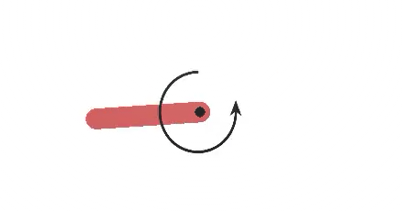
\includegraphics[width=13cm, keepaspectratio]{images/results/pendulum.png}
                        \caption{A representation of the Inverted Pendulum environment. The arc arrow represents the torque applied by the Agent.}
                        \label{fig:results_pendulum}
            \end{figure}
            The chosen environment is Inverted Pendulum. In this environment, a pole is hooked up to a fixed torque at one of its extremities and it is able to rotate using the torque as center of the rotation, describing a full circle. Gravity is applied to the pole at any istant, thus in absence of other forces the pole is drawn to the down-vertical position, at $\frac{3}{2}\pi$. At each time-step, the Agent is able to express a torque force to the pole, allowing it to swing around its rotation center, with the goal of bringing it to the up-vertical position, at $\frac{1}{2}\pi$. \newline
            At each time-step $t$, the state of the environment $s_t$ is represented by a 3-dimensional vector containing the cosine of the pole, the sin of the pole angle and it angular velocity. The Agent is able to express the torque force by controlling a scalar continuous action $a_t$, which values ranges between $-2$ and $2$. Negative action values indicates a torque in the opposite rotation direction. The Agent also receives a negative reward signal $r_t$ which is computed as a function of both pole position and the absolute value of the action chosen by the Agent, in such a way that position distant to up-vertical and higher intensity actions are penalized. Thus, the Agent objective is to swing the pole to bring it to the up-vertical position with a low intensity action, which in turn can be translated in the ability to reach the unstable equilibrium of the up-vertical position and mantain it. The Inverted Pendulum implementation has been provided by the Python OpenAI Gym Library and it has been used without any modifications. \newline
            Two are the main reason for chosing this environment. The first is concerned with the precision of action selections it requires: the goal position is an unstable equilibrium, thus the agent not only must understand how to apply the torque to reach the position, but it also needs to be precised enough to maintain it until the end of the episode. Slight errors in the action selection may bring the pole down lowering the Agent performances significantly and the presence of delay is enhancing this property. The second reason resolves on the fact that the Agent is able to observe states that are composed by sin and cosine values, resulting from the same angle: the module needs to be able to output sufficiently precise state or belief representation to identify the Agent position, if not so, a given predicted state may not even be part of the State Space of the environment, hindering the policy learning process.
            
        \subsection{Simulated Delay Implementation}
        \label{sub:simulated_delays}
        % Dedicated to explain the Delay implementation
        %   - Deterministic Delay
        %   - Stochastic Delay
            As explained in Chapter \ref{chp:ow}, the presence of delays is simulated upon the environment. In practice, a wrapper is implemented around the environment and, at each-time step, it samples the amount of delay $d_t$, or simply $d$ in the case of deterministic delays, and manages the construction of the current extended state $i_t$ as well as the computation of the delayed reward signal $r_t$. Furthermore, it also manages the initialization of the environment: with the presence of delay, the Agent cannot have immediate access to the extended state at the first time-step of the episode, due to the fact that first state is not yet observed. Thus, we need to simulate the first $d$ steps by selecting $d$ random actions, until the first state is observed and the first extended state can be built unifying it to the sequence of actions. During this process, the delay is always assumed a integer multiple of the single time-step.
            
            \subsubsection{Deterministic Delays}
                Deterministic delays implementation is straightforward. The delay wrapper initialize the environment by selecting $d$ random actions for $d$ time-steps, storing the sequence of $d$ states $(s_0, s_1, ..., s_{d-1})$ that the Agent can not observe yet and the correspondent sequence of rewards $(r_0, r_1, ..., r_{d-1})$. At time-step $d$, the wrapper is able to build the first extended state $i_0 = (s_0, a_0, ..., a_{d-1})$, which is observed by the Agent as the first observation, along with the delayed reward signal $r_0 = \mathbf{R}(s_0, a_0)$. After the initialization, at each time-step $t$, the delay wrapper manages the extended states by continuosly updating the observed states, managing the actions and rewards queues. The number of time-step of delay $d$ simulated by the delay wrapper is considered as a parameter of the environment.
            
            \subsubsection{Stochastic Delays}
                Stochastic delays are implemented by means of a jump process, a stochastic process characterized by discrete steps, called jumps. The process is defined by a positive initial delay value $d_0$, a maximum delay value $d_{max}$ and the probability of having a negative jump $p$, reducing the amount of delay. At each time-step $t$, the jump process is sampled by computing the jump and adding it to the current value, thus retrieving the new delay value. The jump also dictates the number of observation the Agent at each time-step: $1-jump$; creating three possible scenarios:
                \begin{itemize}
                    \item If the jump is equal to 0, the Agent will receive only one new observation, thus shifting the extended state as if the delay was deterministic.
                    \item If the jump is greater than zero, the Agent will receive a "negative" amount of observations, meaning that the Agent will not get new observations for a certain number of time-steps, thus enlarging the current extended state.
                    \item If the jump is less than zero, the Agent will receive a set of observations at once. The latest observation of the set will be used to build the next extended state, which dimension will be reduced. 
                \end{itemize}
                In order to control the behaviour of the stochastic delay process, we use $p$ as a parameter of the environment. The range of possible values for $p$ lies between 0.51 and 0.99. Infact, with $p \leq 0.50$, the process would not compute enough negative jumps on average leading it to converge to $d_{max}$; while with $p = 1.00$, the process would constantly compute negative jumps, converging to an undelayed process. 
                
                \begin{figure}[hbtp]
                    \centering
                    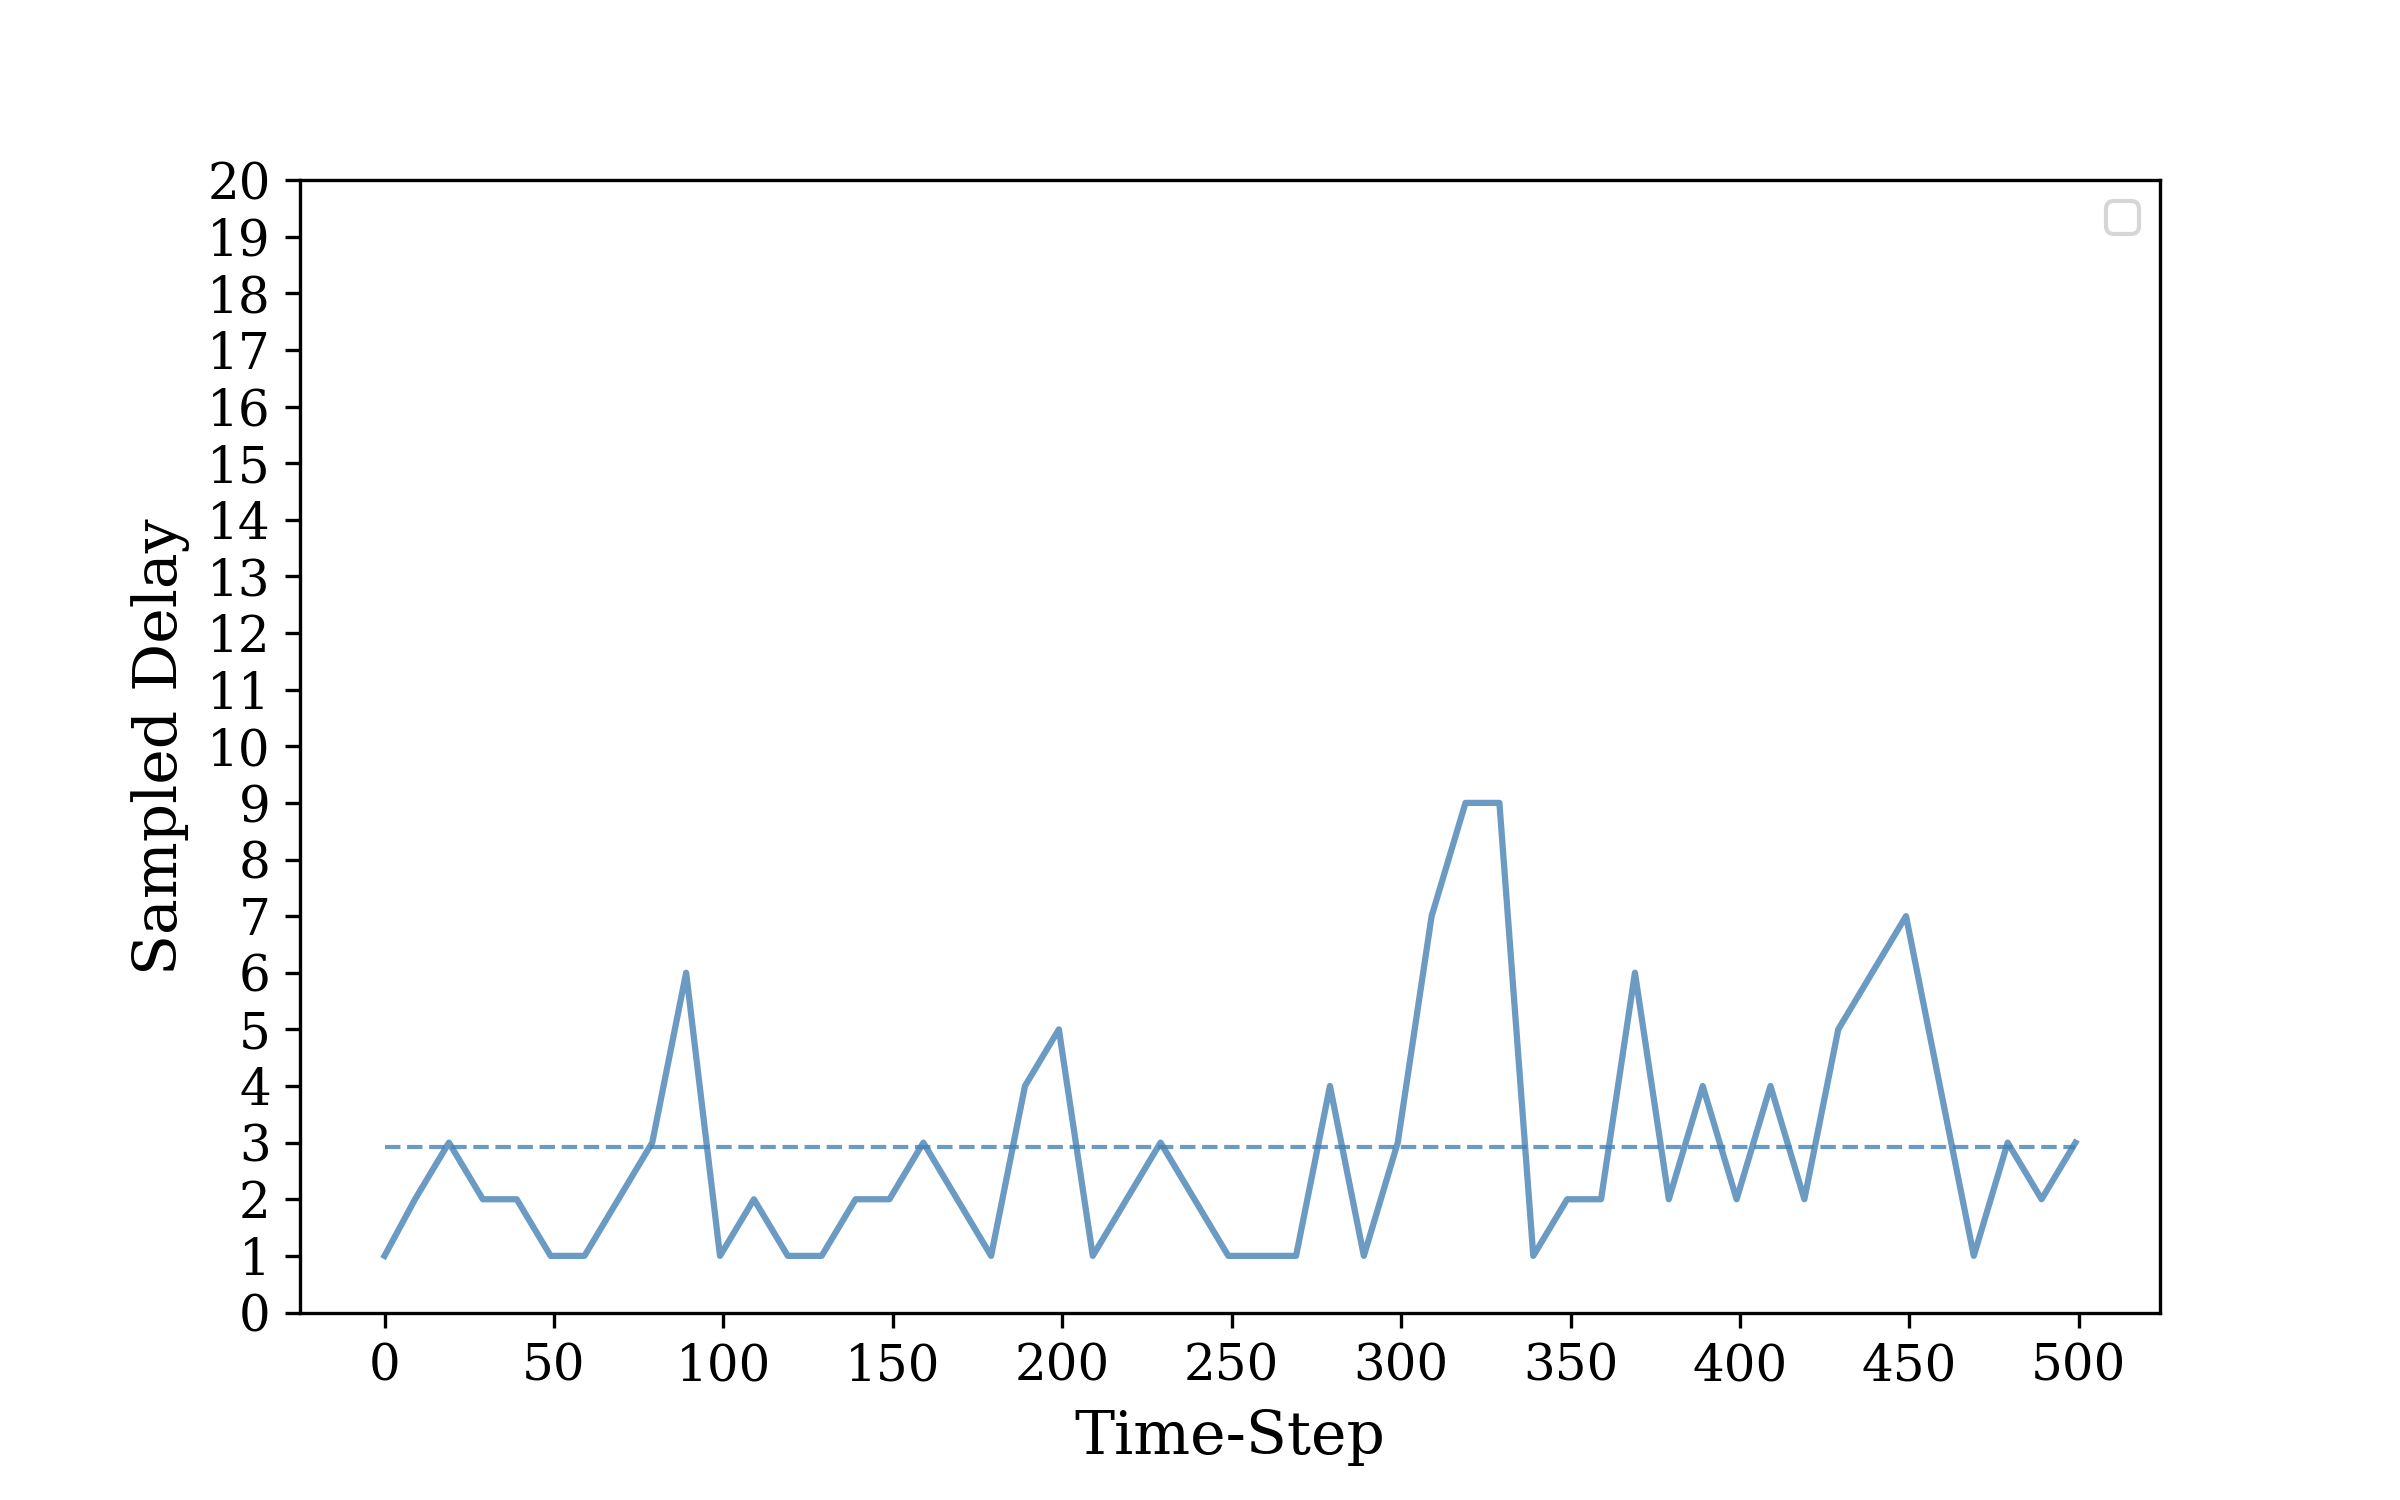
\includegraphics[width=11cm]{images/results/delayp07_sampledelay_1.png}
                    \caption{An instance of the stochastic jump process that generates the amount of delay with $p = 0.7$. The average delay sampled is highlighted by the dashed line.}
                    \label{fig:delayp07_sampledelay}
                    
                    \centering 
                    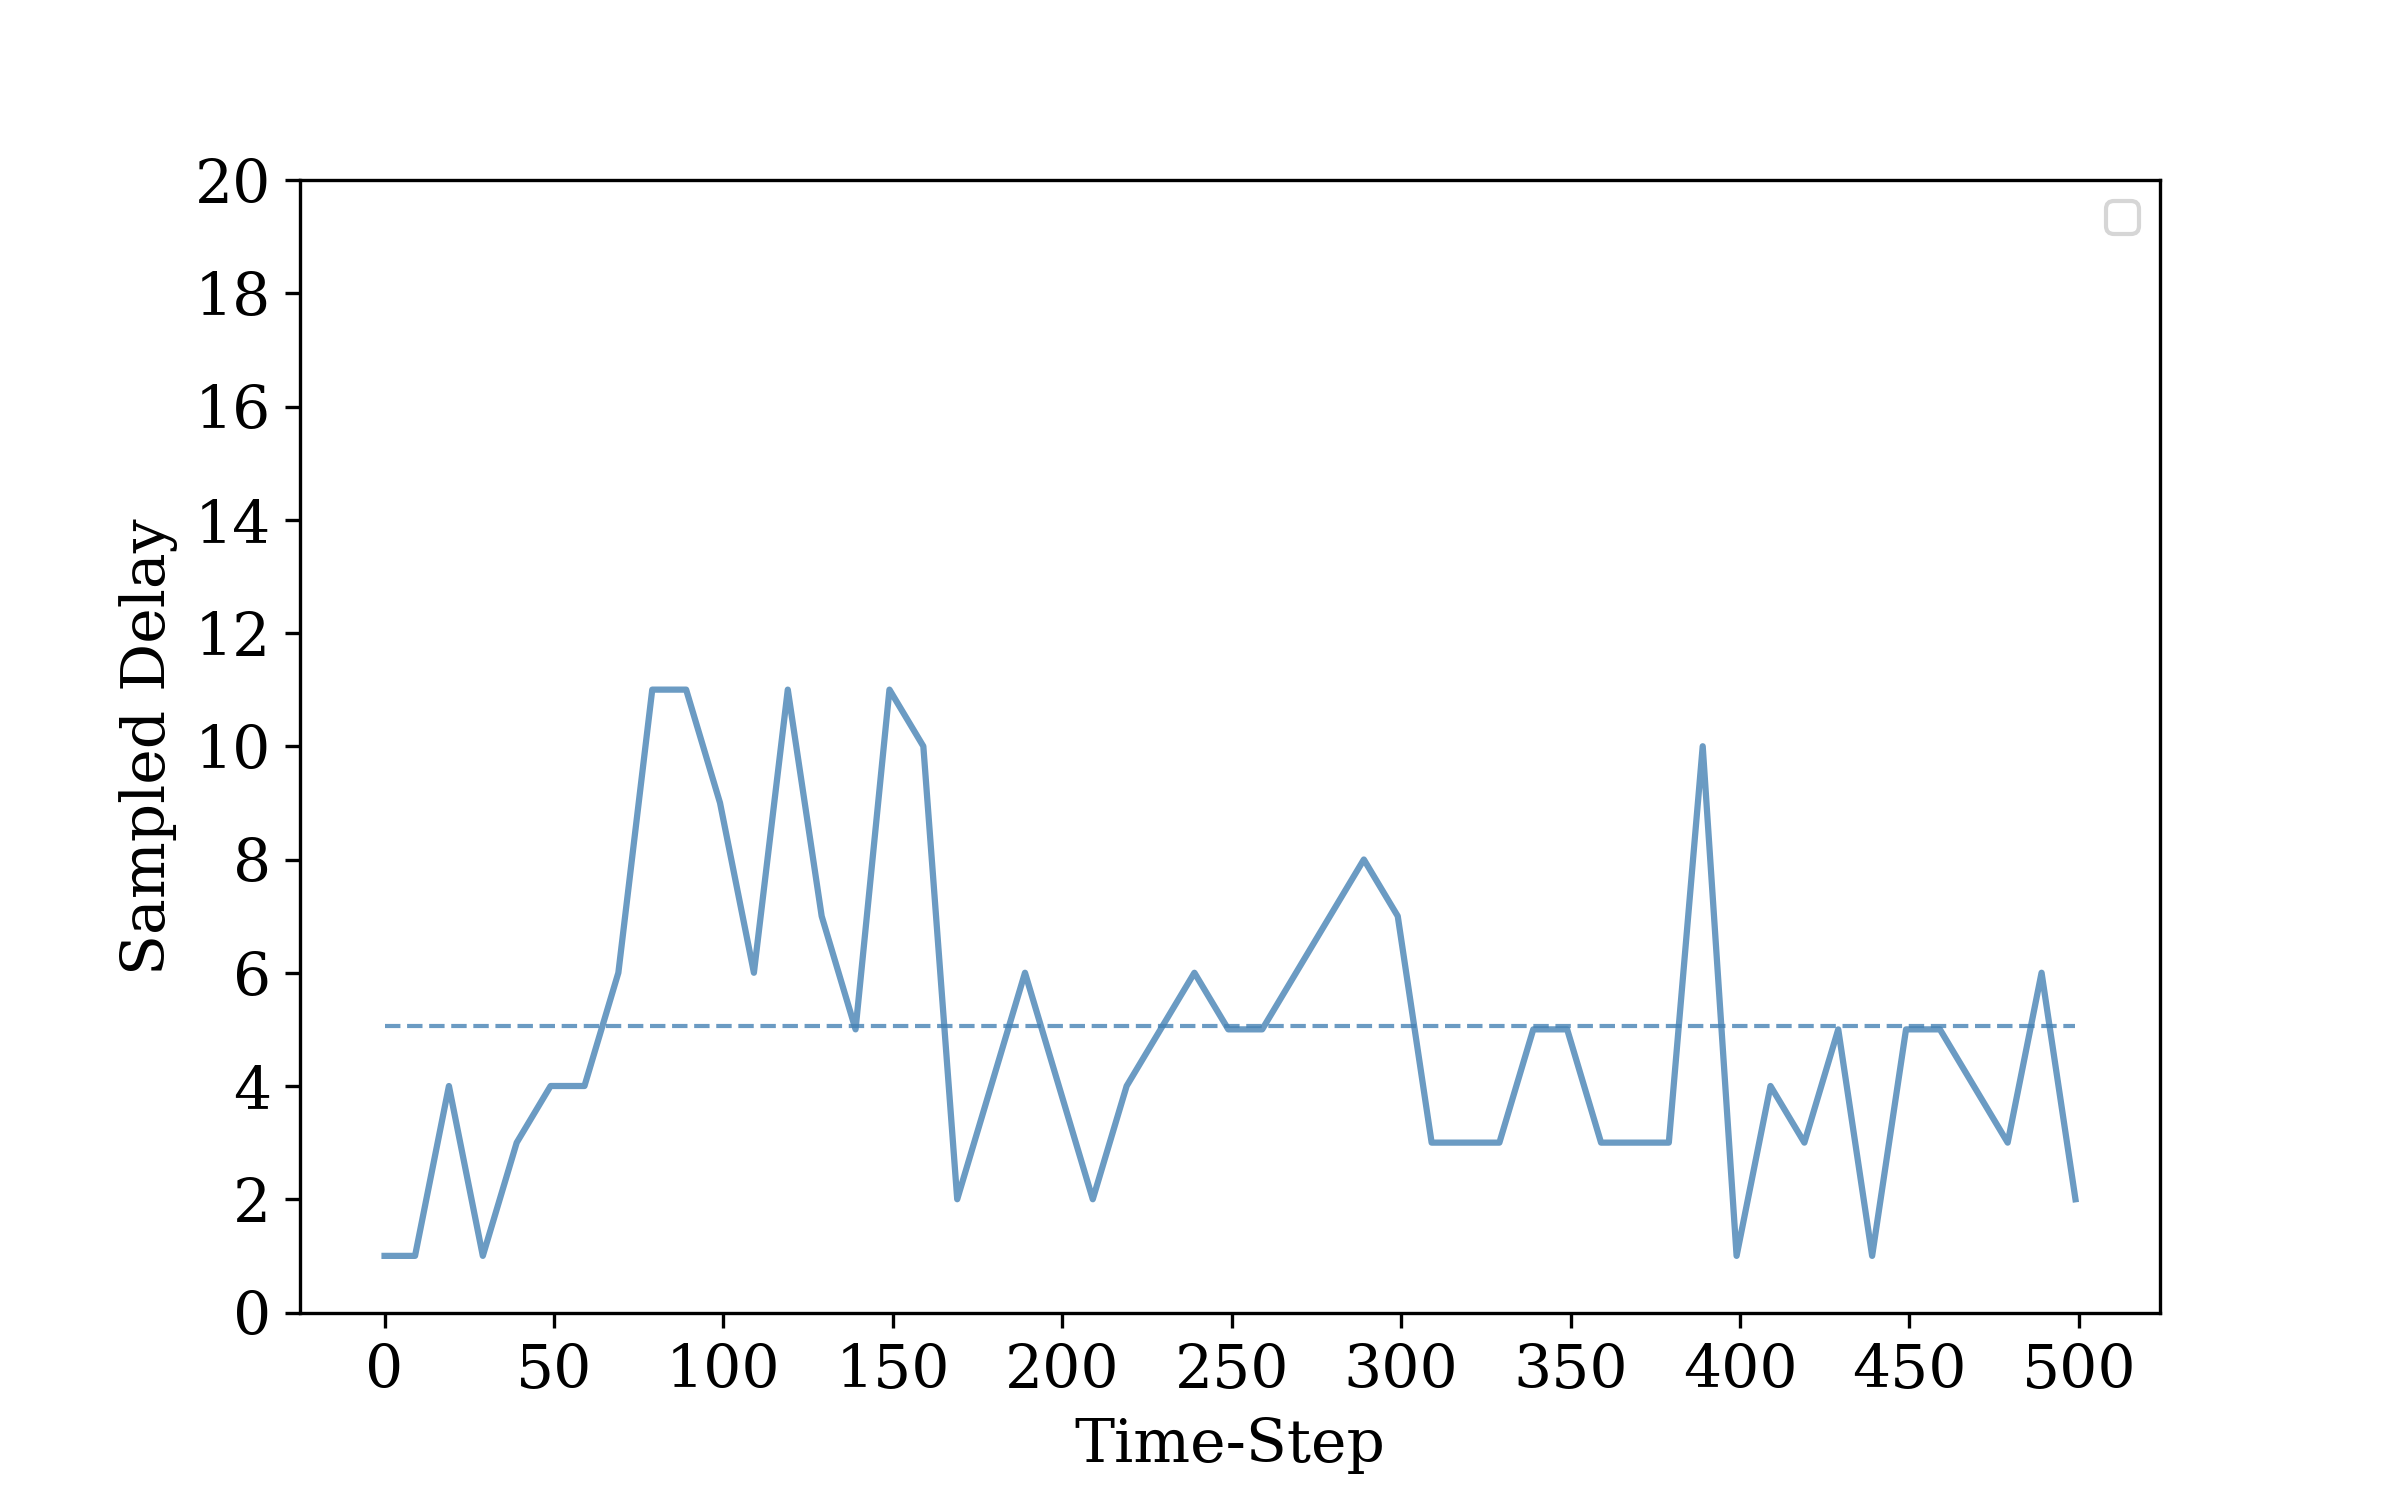
\includegraphics[width=11cm]{images/results/delayp06_sampledelay_1.png}
                    \caption{An instance of the stochastic jump process that generates the amount of delay with $p = 0.6$. The average delay sampled is highlighted by the dashed line.}
                    \label{fig:delayp06_sampledelay}
                    
                    \centering
                    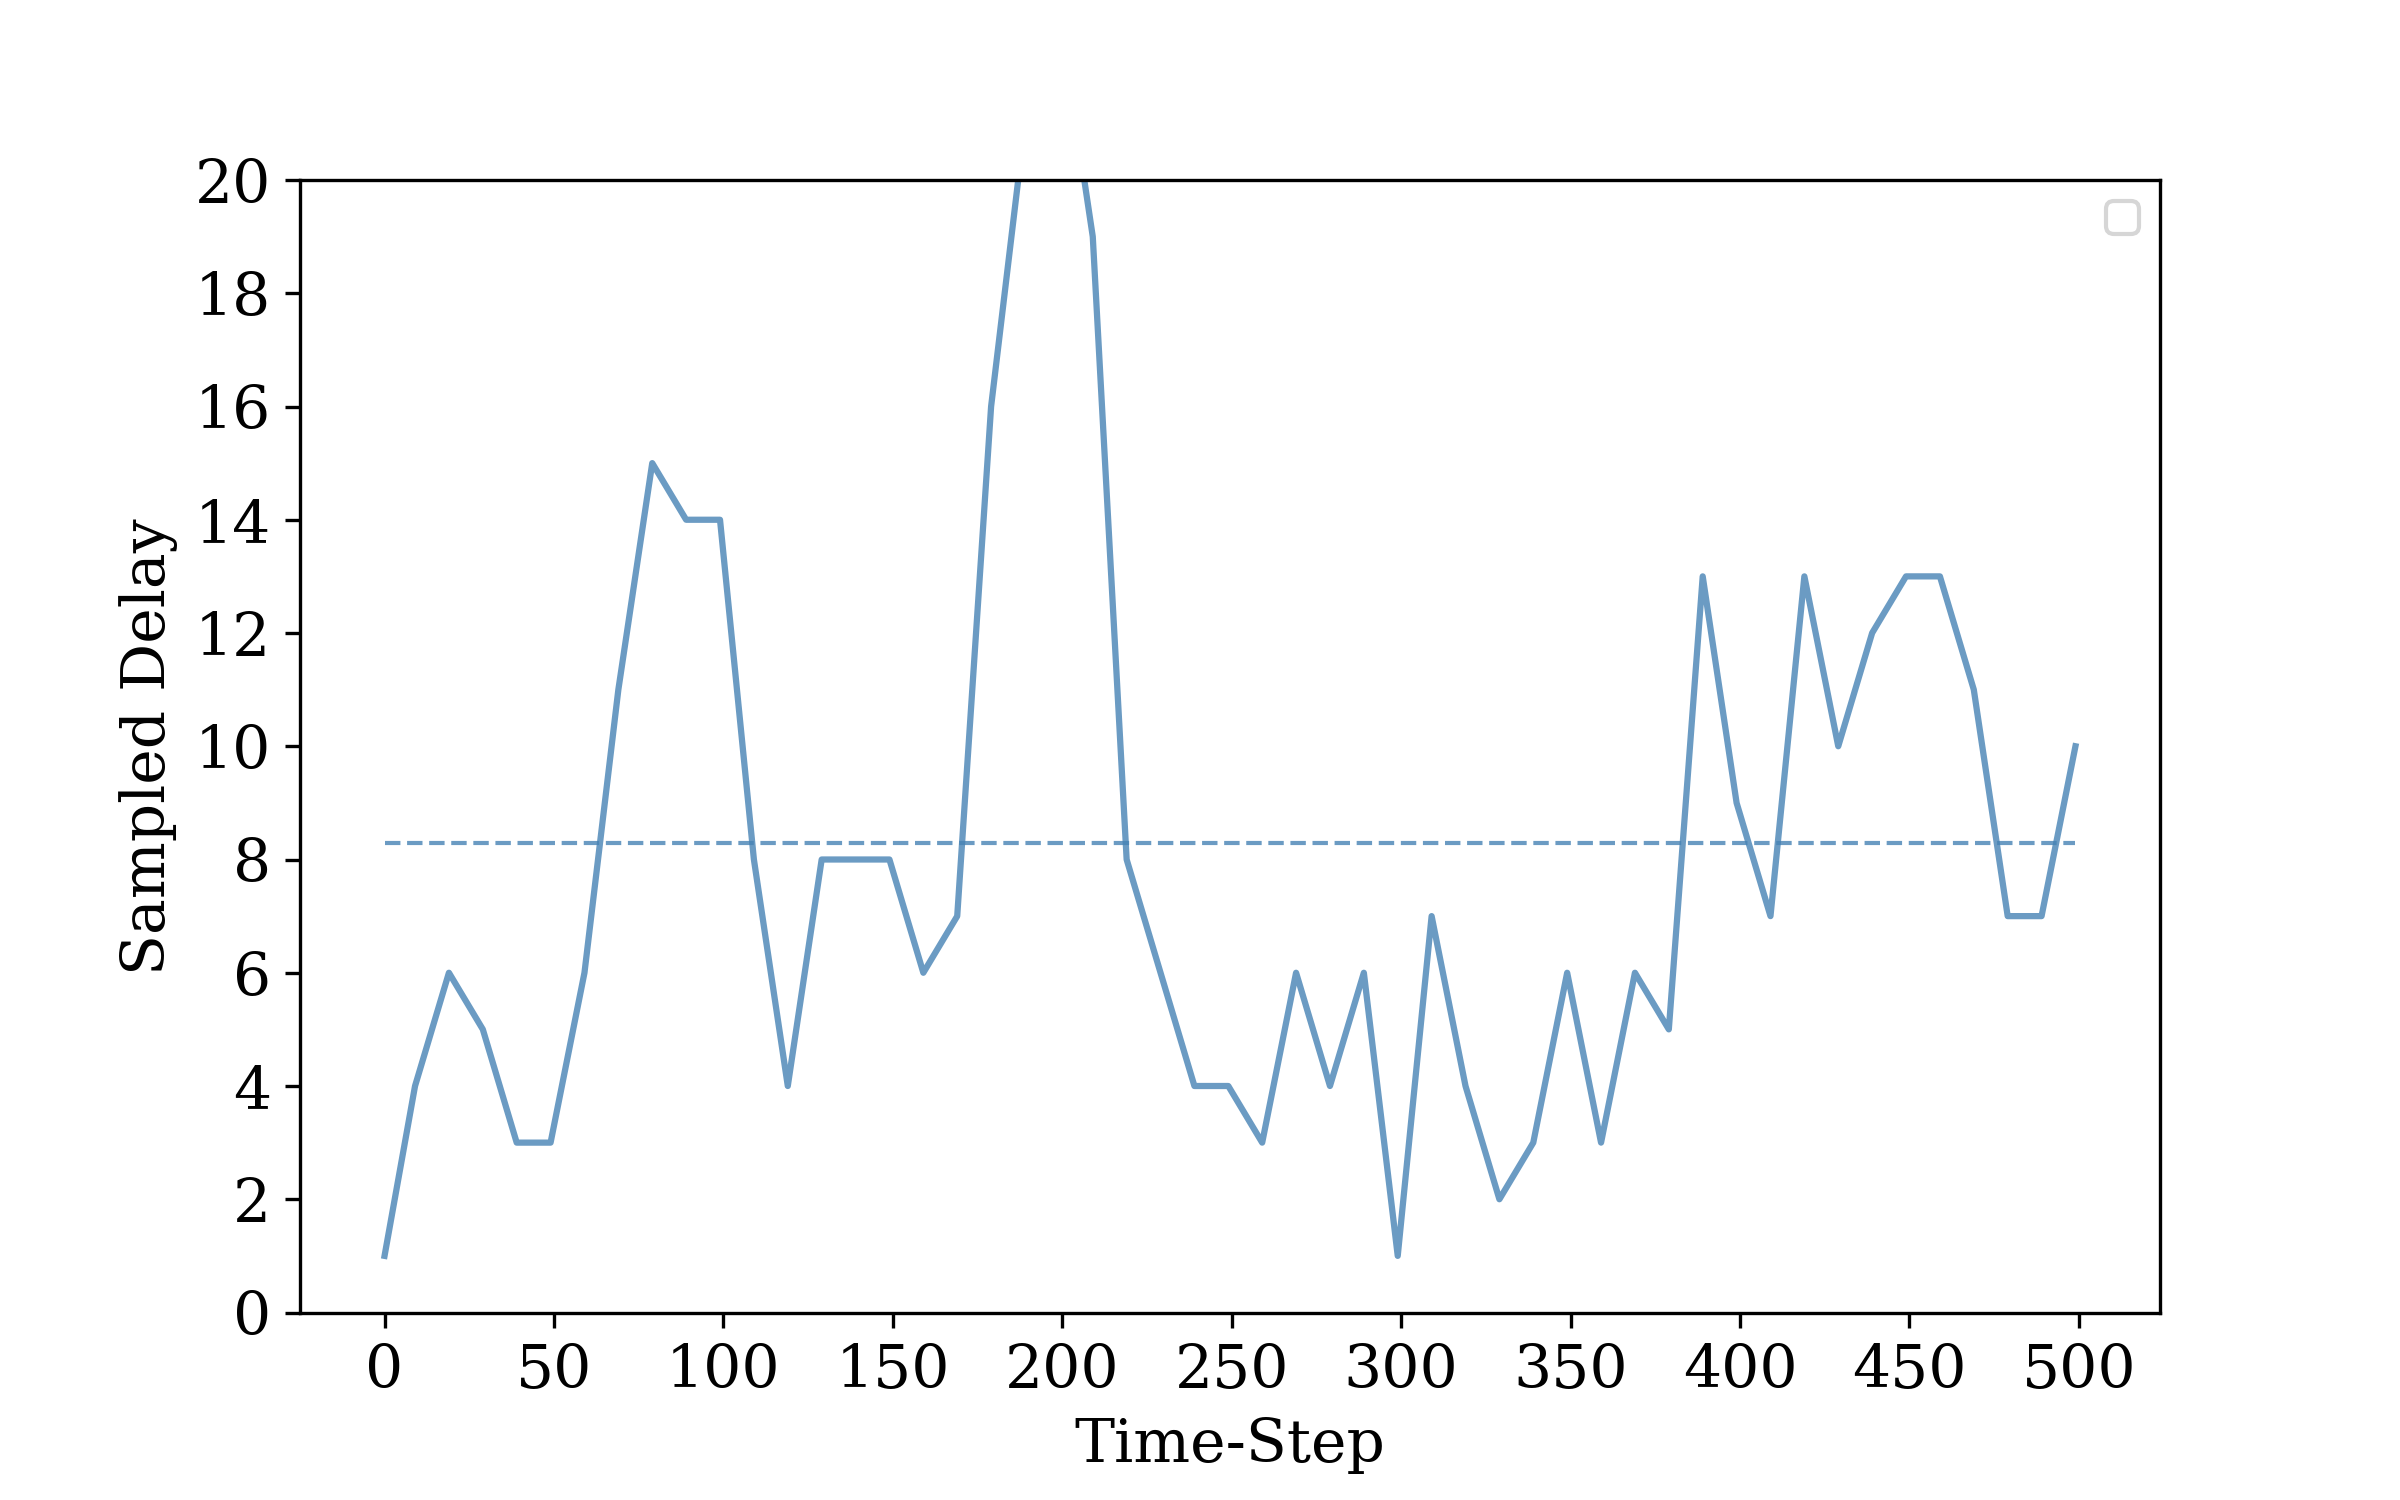
\includegraphics[width=11cm]{images/results/delayp05_sampledelay_1.png}
                    \caption{An instance of the stochastic jump process that generates the amount of delay with $p = 0.5$. The average delay sampled is highlighted by the dashed line.}
                    \label{fig:delayp05_sampledelay}
                \end{figure}
                
        \subsection{Baselines}
        \label{sub:baselines}
        % Dedicated to explain the baseline algorithms used through all tests
            In order to properly estimated the proposed algorithms' performances, we need to define baseline algorithms and evaluate their performance in the same context. However, given the presence of delays, standard state-of-the-art Reinforcement Learning algorithm cannot be directly deployed as baselines. They need to be adapted through one of the approaches dedicated to the DMDP framework, presented in Section \ref{sota:delay_approaches}. We decided to adapt TRPO algorithm to the augmented and memoryless approach to have a direct comparison with our model-based approach of L2-TRPO and D-TRPO. We also implemented SARSA and D-SARSA as additional memoryless approach baselines. \newline
            It is important to mention that none of these algorithms is able to cope with stochastic delays, due to the structure of the feedforward networks that implement Policy and Value functions, which are not able to handle variable-size inputs. For this reason, experiments involving stochastic delays are only concerned with L2-TRPO and D-TRPO performances.
            
            \subsubsection{Augmented Approach: A-TRPO}
                We refer to TRPO adaptation to the augmented approach as Augmented TRPO or A-TRPO. At each time-step $t$, the Agent observes the extended state $i_t$, selects an action $a_t$, action $a_{t-d}$ is executed and the Agent receives the delayed reward $r_t = \mathbf{R}(s_{t-d}, a_{t-d})$. In practice, TRPO algorithm is deployed to learn upon the augmented MDP resulting from the original DMDP, as explained in Section \ref{subs:augmentedapproach}. TRPO implementation is the same used for L2-TRPO and D-TRPO.
                
            \subsubsection{Memoryless Approach: M-TRPO}
                We refer to TRPO adaptation to the memoryless approach as Memoryless TRPO or M-TRPO. At each time-step $t$, the Agent observes the state $s_{t-d}$, selects an action $a_t$, action $a_{t-d}$ is executed and the Agent receives the delayed reward $r_t = \mathbf{R}(s_{t-d}, a_{t-d})$. Thus, TRPO is deployed to learn action selection in the environment observing only the last known state, ignoring the presence of delay, as explained in Section \ref{subs:memorylessapproach}. TRPO implementation is the same used for L2-TRPO and D-TRPO.
                
                
            \subsubsection{Memoryless Approach: SARSA and d-SARSA}
            % Note: Discretized State Space
                At last, we wanted to compare our original algorithms against a specific algorithm from the literature. We chose D-SARSA, presented in Section \ref{subs:memorylessapproach}, as a memoryless algorithm that achieved good results. Along with it, given its easy implementation, we also decided to test the original SARSA algorithm in the context of memoryless approach. \newline
                In order to deploy SARSA and D-SARSA with environments characterized by continuous state and/or action space, such as Inverted Pendulum, it is necessary to discretize them. In our tests, both SARSA and D-SARSA learns upon a grid-discretized State Space of 15x15x15 and a discretized Action Space of 3 values.
                
                
    \newpage
    \section{Module Parameters Tuning}
    \label{results:module_tuning}
    % Section dedicated to the process of finding which parameters influences Module's performances and most affect the total number of parameter. We want to find the best trade-off, given the fact that each sample will be processed through the Encoder.
    %   - Tests on older version of the Module
    %   - Encoder Dim vs Encoder FF Dim vs Encoder Layers
    %   - Select only relevant plots for the comparison
        The first step in the process of evaluating the original implementation is assessing the modules' properties: which are the hyperparameters that affect performances and total number of parameters the most. The goal of this section is to understand which hyperparameters offer the best trade-off between performance gains and number of additional parameters in the module. Given the fact that the modules are involved in computing the state or belief representation at each time-step, optimizing the total number of parameters is a key factor in order not to slow down the training process to a point in which the modules' benefits are sinked by long training times. \newline
        The following tests are performed on the State-Prediction module, which is trained for 200 epochs, each composed by 100 trajectories of 250 steps, for a total of 5 million steps. Each module has been trained 3 times with 3 different seeds, the results are presented as averages between them. In order to concisely refer to each of the modules tested, we set up a bit of nomenclature: each module will be referred to as [$enc_{ff}$, $enc_{dim}$, $e$]. 
        
        \subsection{Cross-Validation}
        % Describe the first test with all Encoders between [16, 16, 1] and [32, 32, 2]
            In this test, we start with two reference modules [32, 32, 2] and [16, 16, 1] and we evaluate the performance difference between them and the sequence of modules obtained by lowering one hyperparameter at a time: [16, 32, 2]; [32, 16, 2] and [32, 32, 1]. Figure \ref{fig:results_parametertuning_1} shows the results of the test and Figure \ref{fig:results_parametertuning_2} focuses on the last epochs of training for a better illustration of the differences between the modules. \newline
            As expected, modules [16, 16, 1] and [32, 32, 2] a respectively the worst and best modules performance-wise, but [32, 32, 2] also has approximately 7 times the number of parameters. As for the other tested modules, we can break down conclusions for each of them:
            \begin{itemize}
                \item Module [16, 32, 2] with 12227 parameters: lowering $enc_{ff}$ from 32 to 16 does not affect the module performance-wise and results in a loss of 14.5\% parameters, possibly indicating that $enc_{ff}$ is not crucial for the modules capabilities.
                \item Module [32, 16, 2] with 4483 parameters: lowering $enc_{dim}$ from 32 to 16 hugely affects the module's performances, which become closer to [16, 16, 1] then any other module, possibly indicating that the parameter plays a very important role in the module capabilities. As expected, since $enc_{dim}$ directly affect the matrices' dimensions in the Self-Attention network, the number of total parameter is greatly reduced by 65.9\%.
                \item Module [32, 32, 1] with 7843 parameters: lowering the number of encoder layers has a mild effect on module's performances, with a loss of 45.2\% of the parameters, possibly indicating an intermediate importance between the other two parameters.
            \end{itemize}
            
            From the results of these tests, we can state that $enc_{dim}$ and $e$ are influencing both module's performances and total number of parameters significantly, while $enc_{ff}$ is not as influential and it may be decresed in favor of less total parameters. Looking at the module design, this result is reasonable: $enc_{dim}$ directly affects the number of parameters used to compute the attention scores, while $e$ determines how many encoder layers are used on top of each other. However, even if lowering $enc_{dim}$ has impacted performances more, we also need to observe that the total number of parameters has also diminished drastically. The next Section is concerned with a test to properly assess which of the two parameters offer the best trade-off between computational complexity and performances.
        
        \subsection{Performance Scaling Test}
        % Describe the second test between [8, 192, 2] - 343507; [8, 256, 1] - 336907 and [8, 512, 1] - 1329163
            This second test is aimed at establishing which parameter offers the best trade-off between $enc_{dim}$ and $e$ as well as observing how the module's performances scale with them. For this reason, we test three new modules: [8, 192, 2] with 343507 parameters; [8, 256, 1] with 336907 and [8, 512, 1] with 1329163 parameters. Figures \ref{fig:results_scalability_1} and \ref{fig:results_scalability_2} illustrate the result of this test. \newline
            At first, we focus on [8, 192, 2] and [8, 256, 1]: both modules offer almost the same number of parameters, slightly in favor of $e$ parameter, in contrast to the previous test. However, [8, 256, 1] is clearly faster to learn and it can reach a slightly better loss value, even with few less parameters. Even if the difference is not great, we decide give priority to $enc_{dim}$, also given its meaning within the module's architecture. Also, we can observe that lowering $enc_{ff}$ to 8 hasn't impacted the module's performances in both cases. \newline
            At last, it is possible to observe that module [8, 512, 1] is showing increased speed to convergence and a slightly better loss value, indicating that it is possible to enlarge $enc_{dim}$ to 512 without encountering significant diminishing return effects.
        
        \subsection{ADAM Learning Rate}
            As explained in Section \ref{ow:deterministic_module} and \ref{ow:beliefmodule}, the module is trained using ADAM optimization algorithm. All tests shown so far are executed with a conservative learning rate of 0.0001. After having established the most important parameters performance-wise, we want to decrease the total number of parameters required possibly maintaining the same level of performances, because we realize that a module with so many parameters as in the last test is not tractable in practice. For this reason, we want to test the module [8, 128, 1] with 86539 parameters trained with ADAM with larger learning rates: 0.1, 0.01 and 0.001; and we compare it to the previous trained module [8, 512, 1], trained with learning rate 0.0001. Figures \ref{fig:results_lr_2} and \ref{fig:results_lr_1} show the results of the test. \newline
            In practice, the test shows that we are able to increase ADAM learning rate safely until a value of 0.01, since 0.1 shows lower and unstable performances. Furthermore, [8, 128, 1] is able to outperform [8, 512, 1] significantly with a proper learning rate value, while having a fraction of the total number of parameters.
            
        \subsection{Causal Option}
            As a last test, we want to establish the effects of the causal mask applied to the Self-Attention network of the module. To this purpose, we compare a new module [8, 128, 1] trained with the causal mask to [8, 128, 1] and [8, 512, 1]. Figures \ref{fig:results_causal_1} and \ref{fig:results_causal_2} illustrates the results of the test. \newline We conjecture that the causal mask allows the module to "concentrate" only on the correct portion of the input sequence while computing the attention vectors for each input element, thus avoiding a waste of time and resources by looking at the future elements that are not relevant. Results seems to confirm the hypothesis: the module trained with the causal mask is faster to converge and reaches a slightly better loss value overall.
        
        \begin{figure}[hbtp]
                \centering
                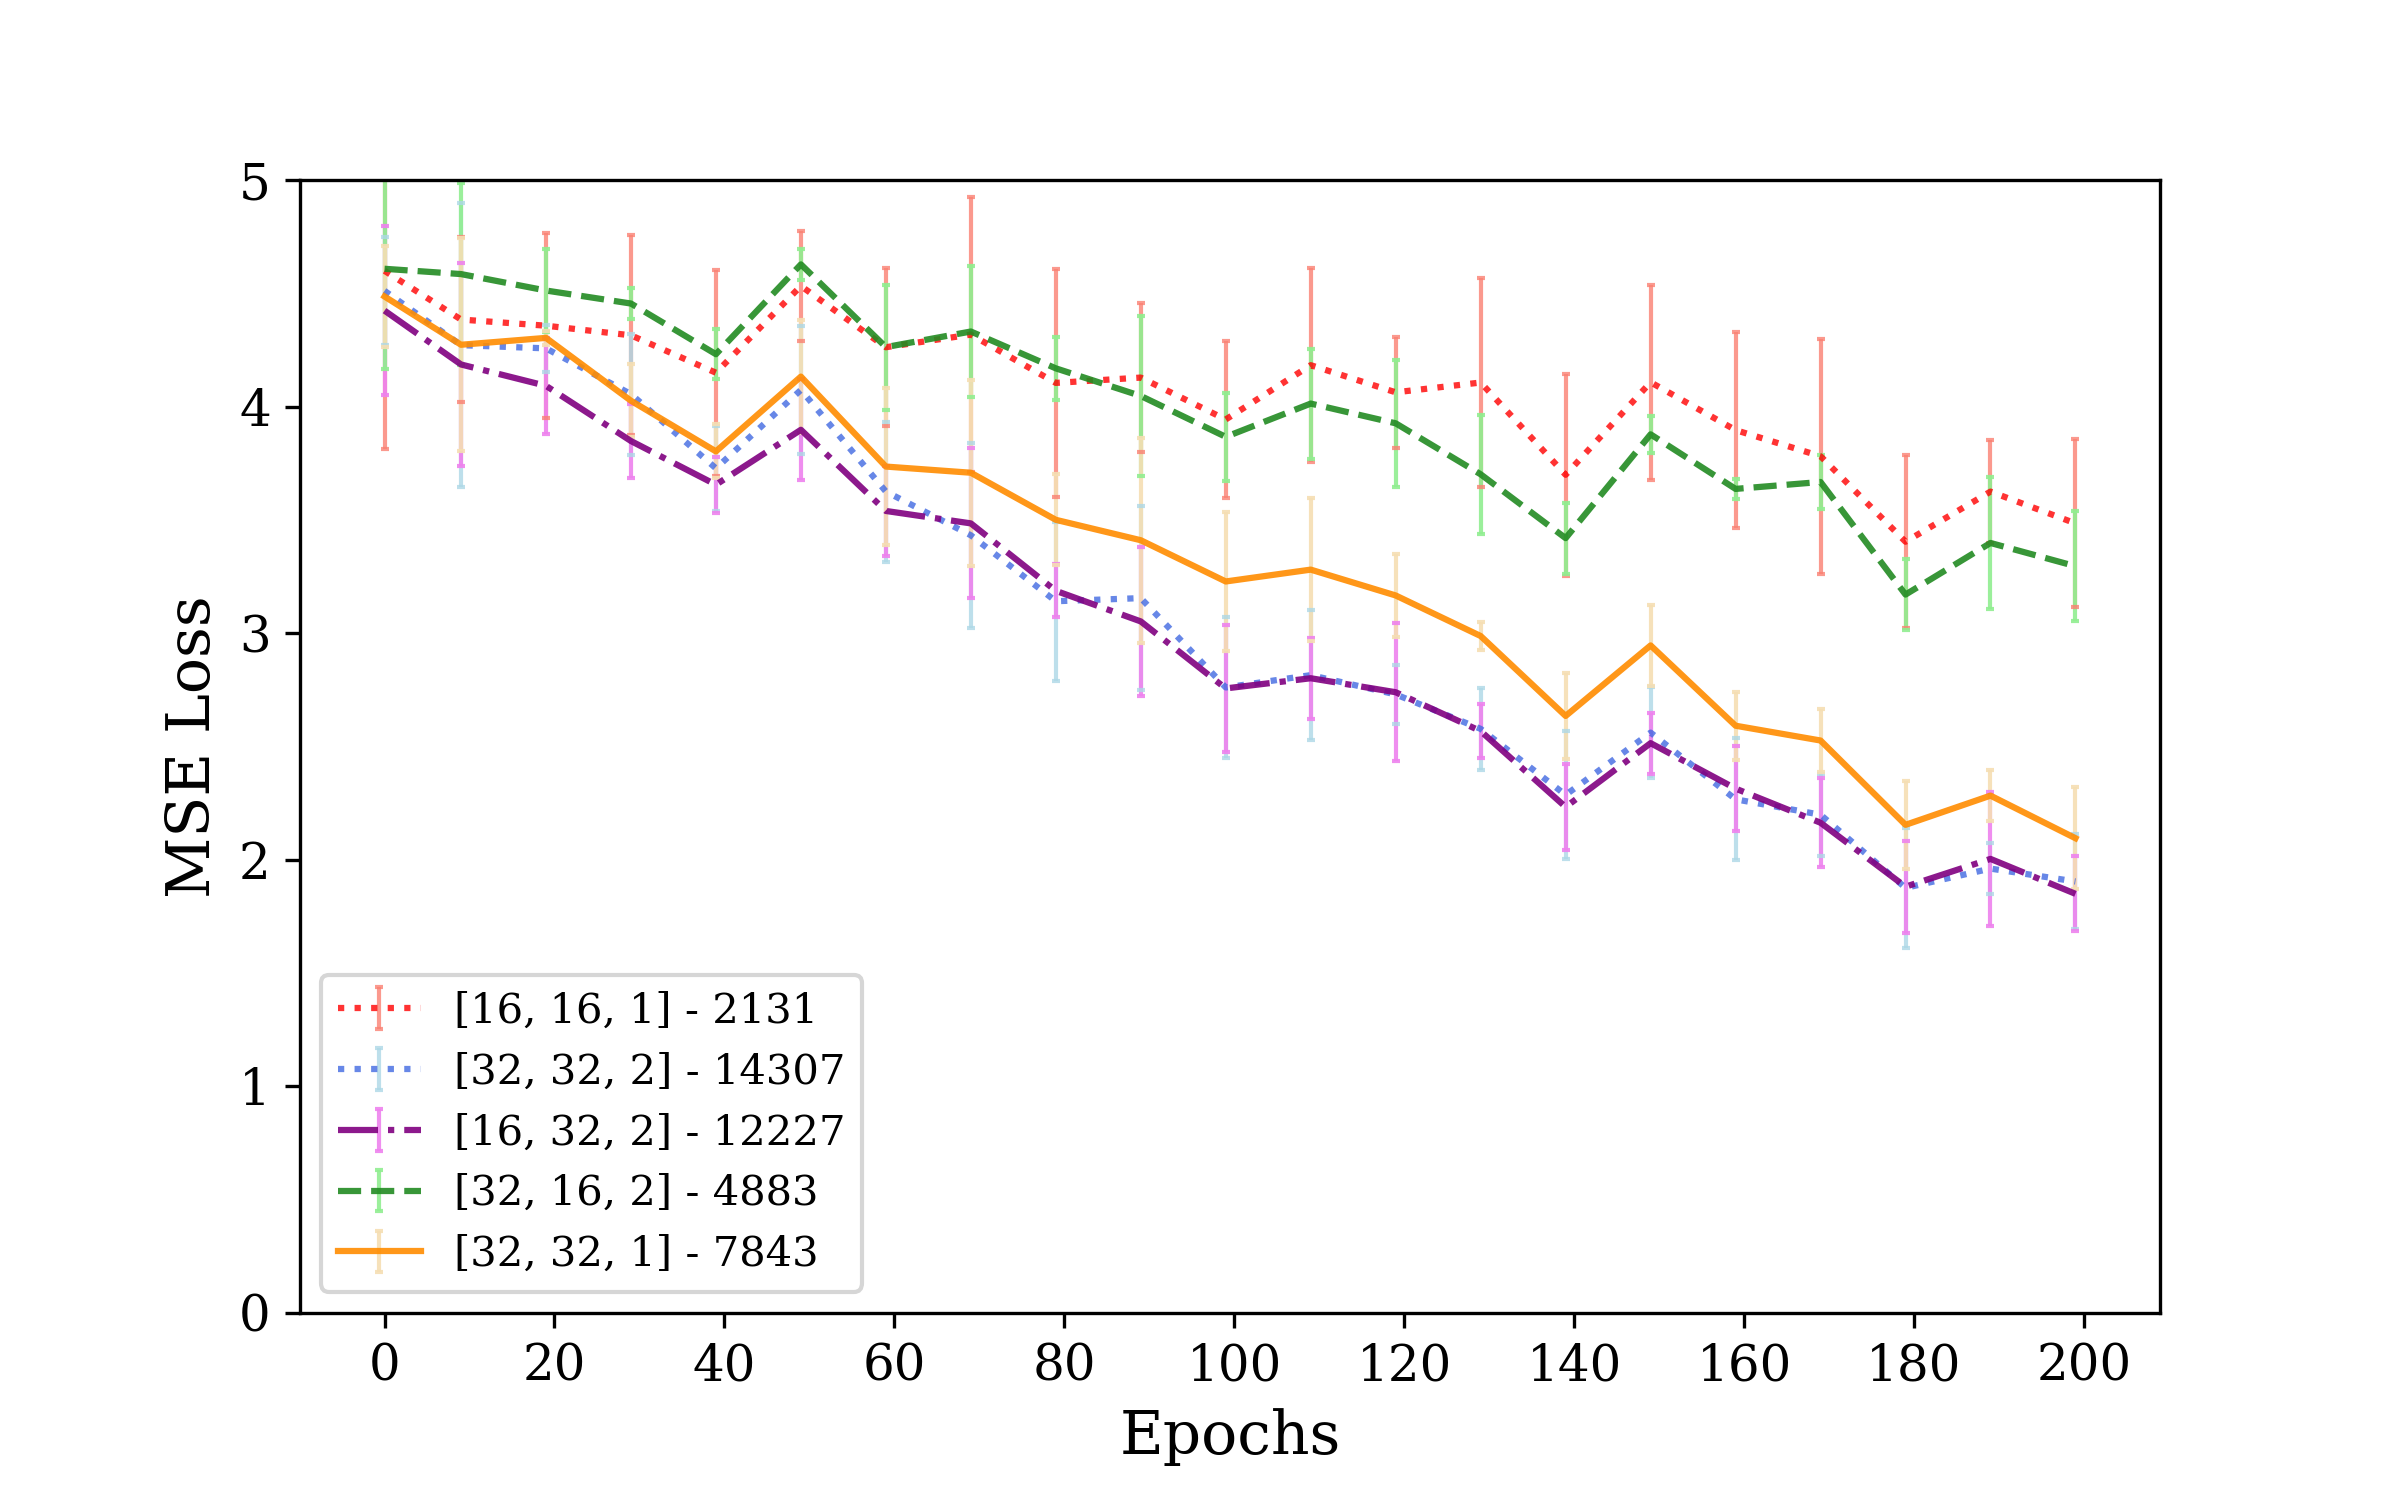
\includegraphics[width=15cm, keepaspectratio]{images/results/module_parametertuning_1.png}
                \caption{MSE Loss Function $L_{pred}$ of the trained modules. The right-hand side number in the legend is the total number of parameter of each module.}
                \label{fig:results_parametertuning_1}
                
                \vspace{1.5cm}
                
                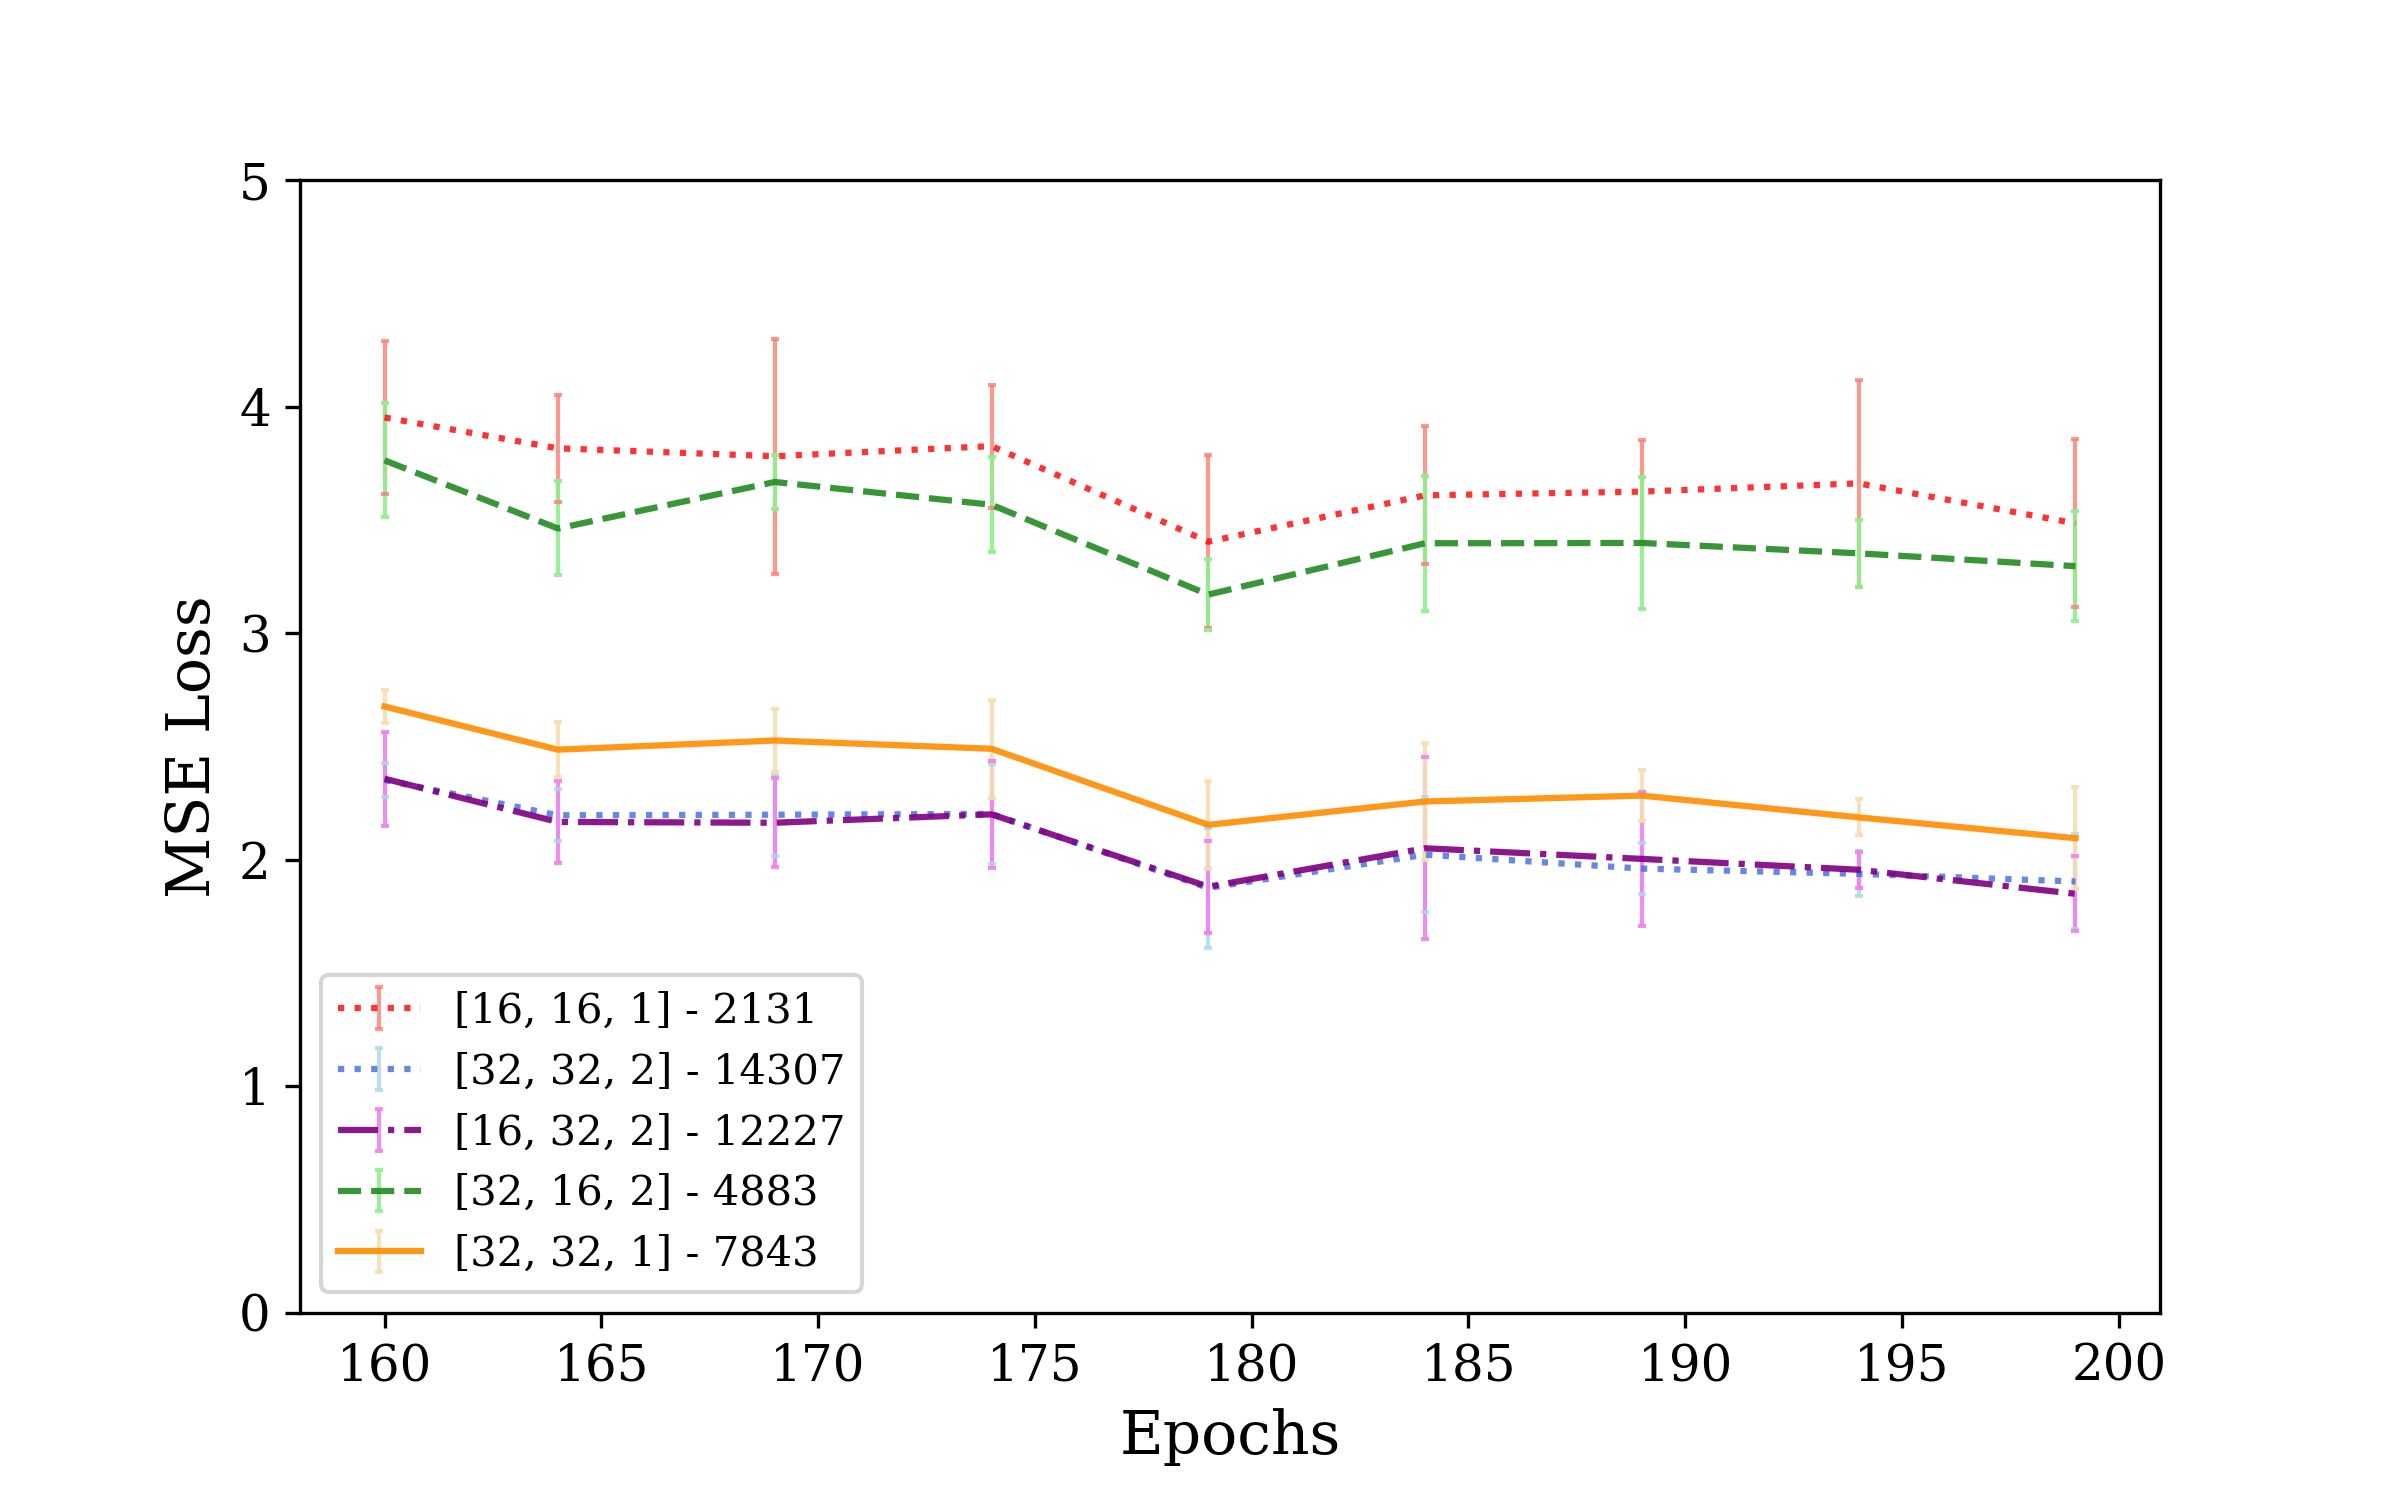
\includegraphics[width=15cm, keepaspectratio]{images/results/module_parametertuning_2.png}
                \caption{MSE Loss Function $L_{pred}$ of the trained modules between Epoch 160 and Epoch 200. The right-hand side number in the legend is the total number of parameter of each module.}
                \label{fig:results_parametertuning_2}
        \end{figure}
        
        \begin{figure}[hbtp]
                \centering
                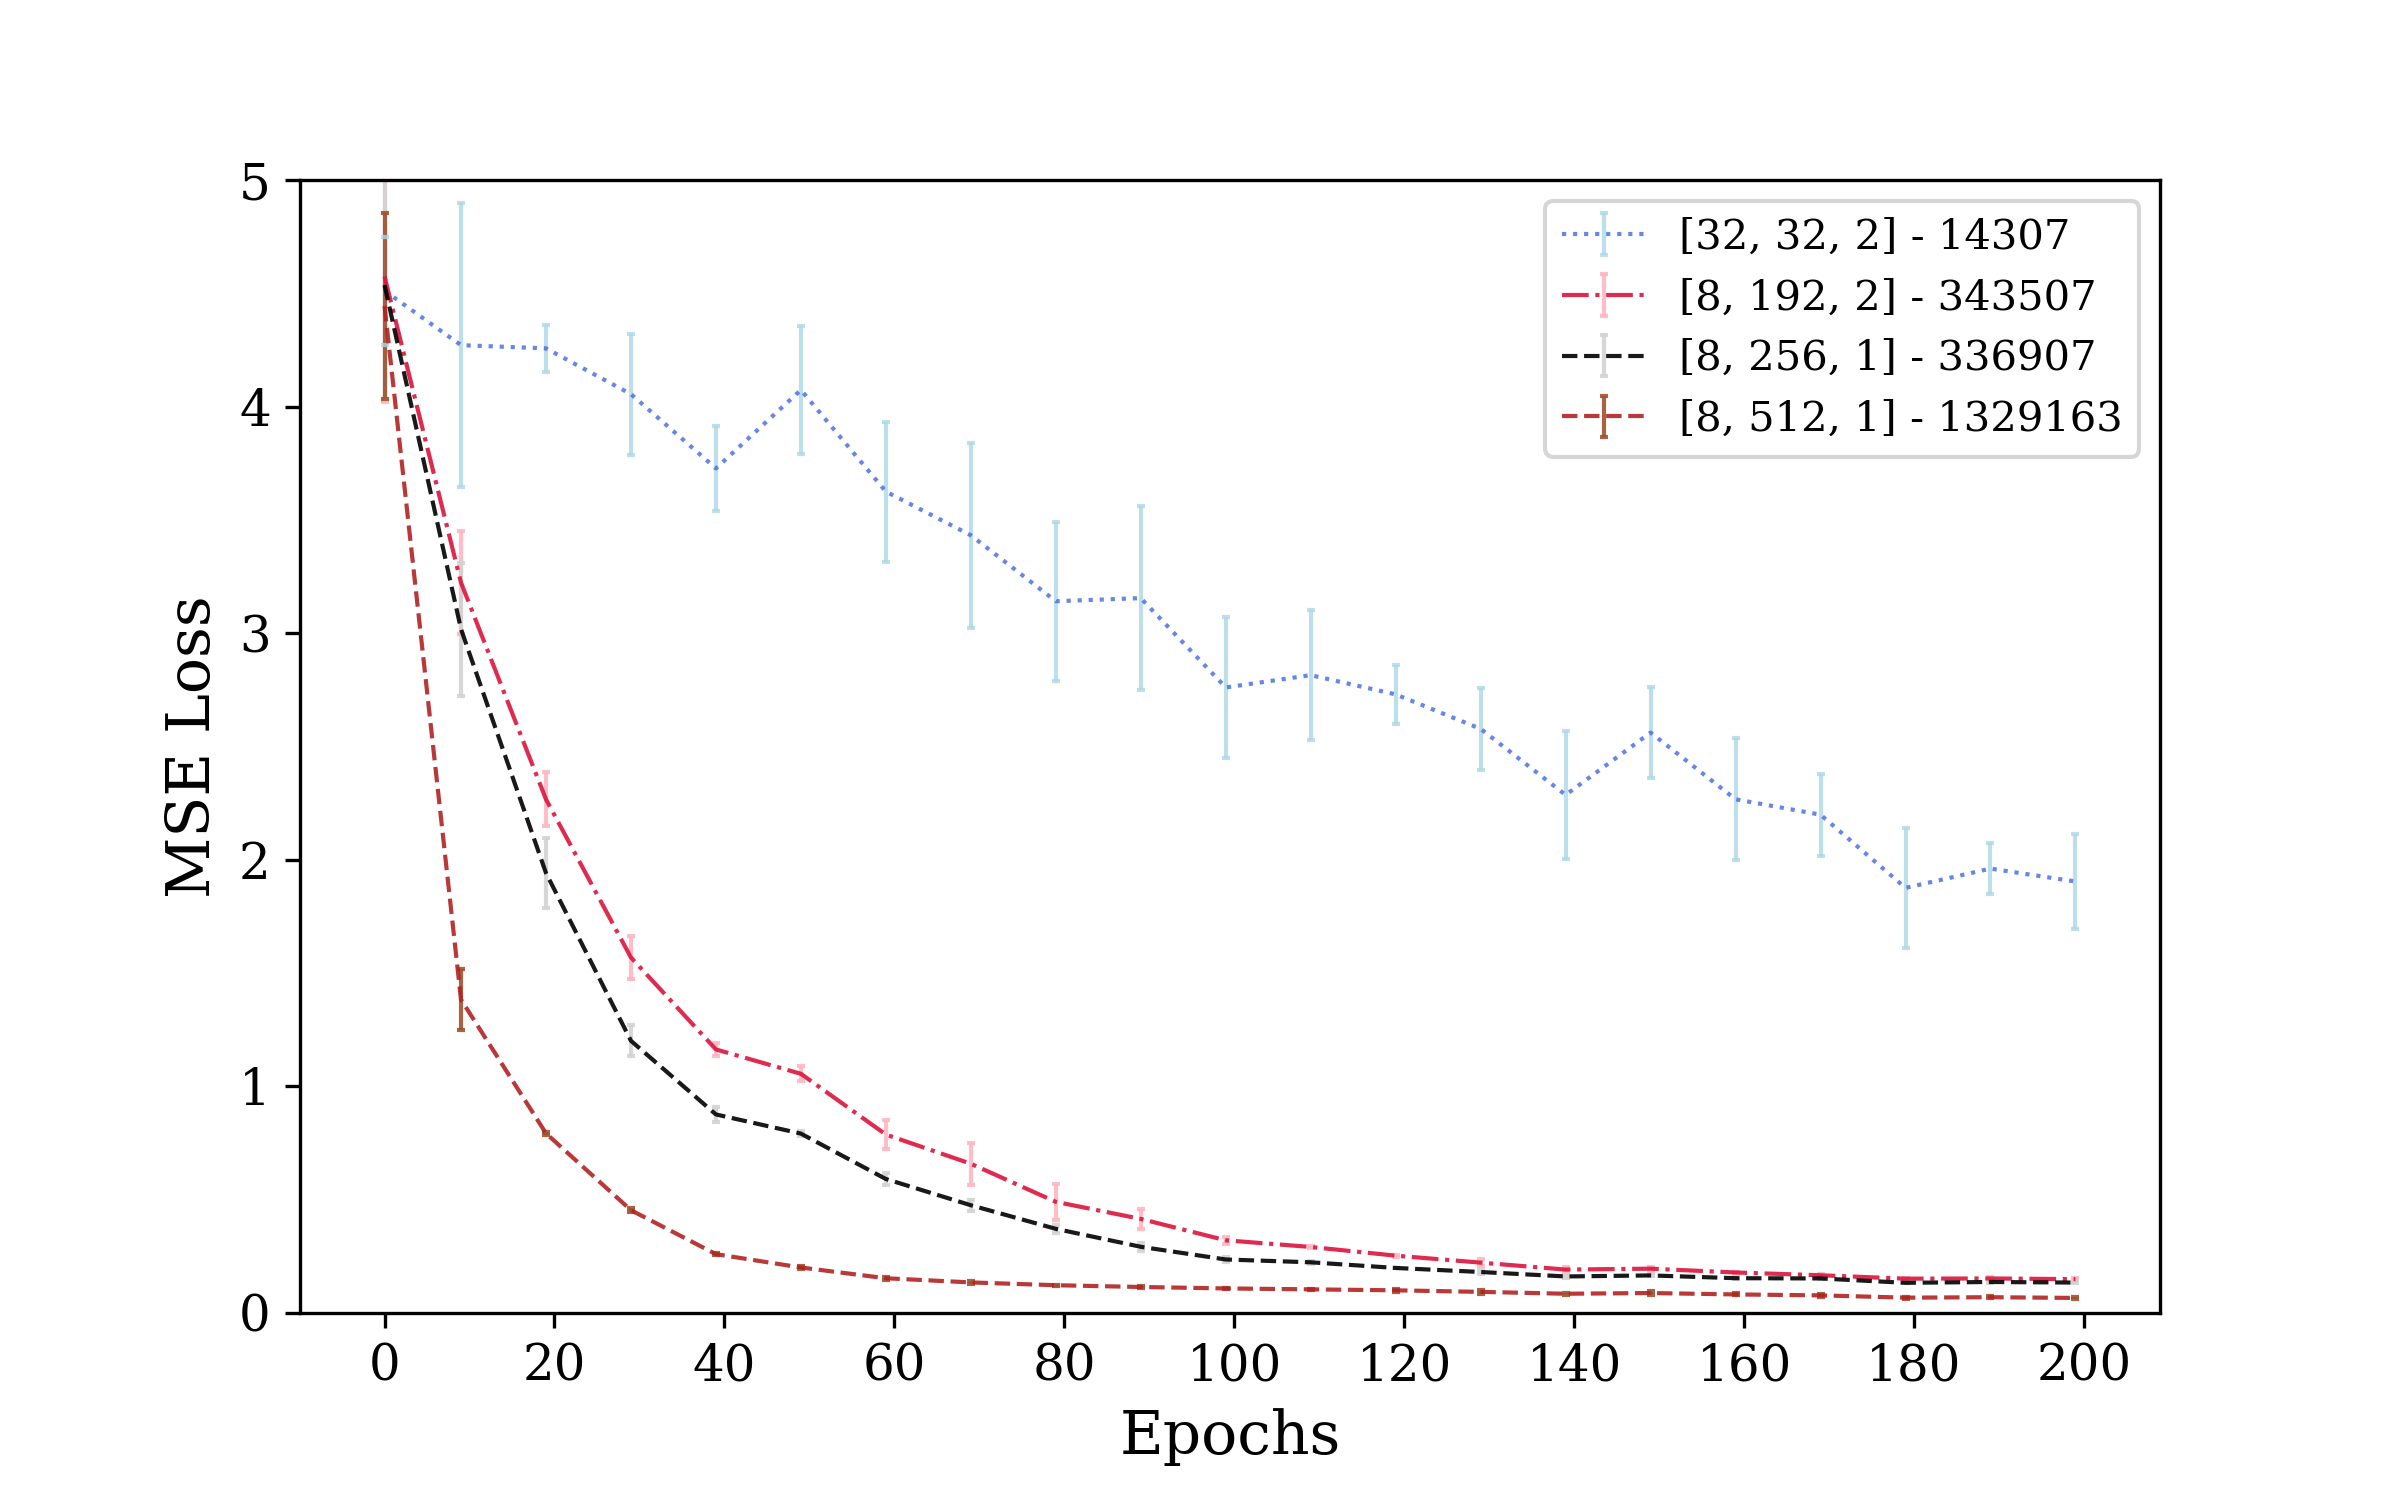
\includegraphics[width=15cm, keepaspectratio]{images/results/module_scalability_1.png}
                \caption{MSE Loss Function $L_{pred}$ of the trained modules. The right-hand side number in the legend is the total number of parameter of each module.}
                \label{fig:results_scalability_1}
                
                \vspace{1.5cm}
                
                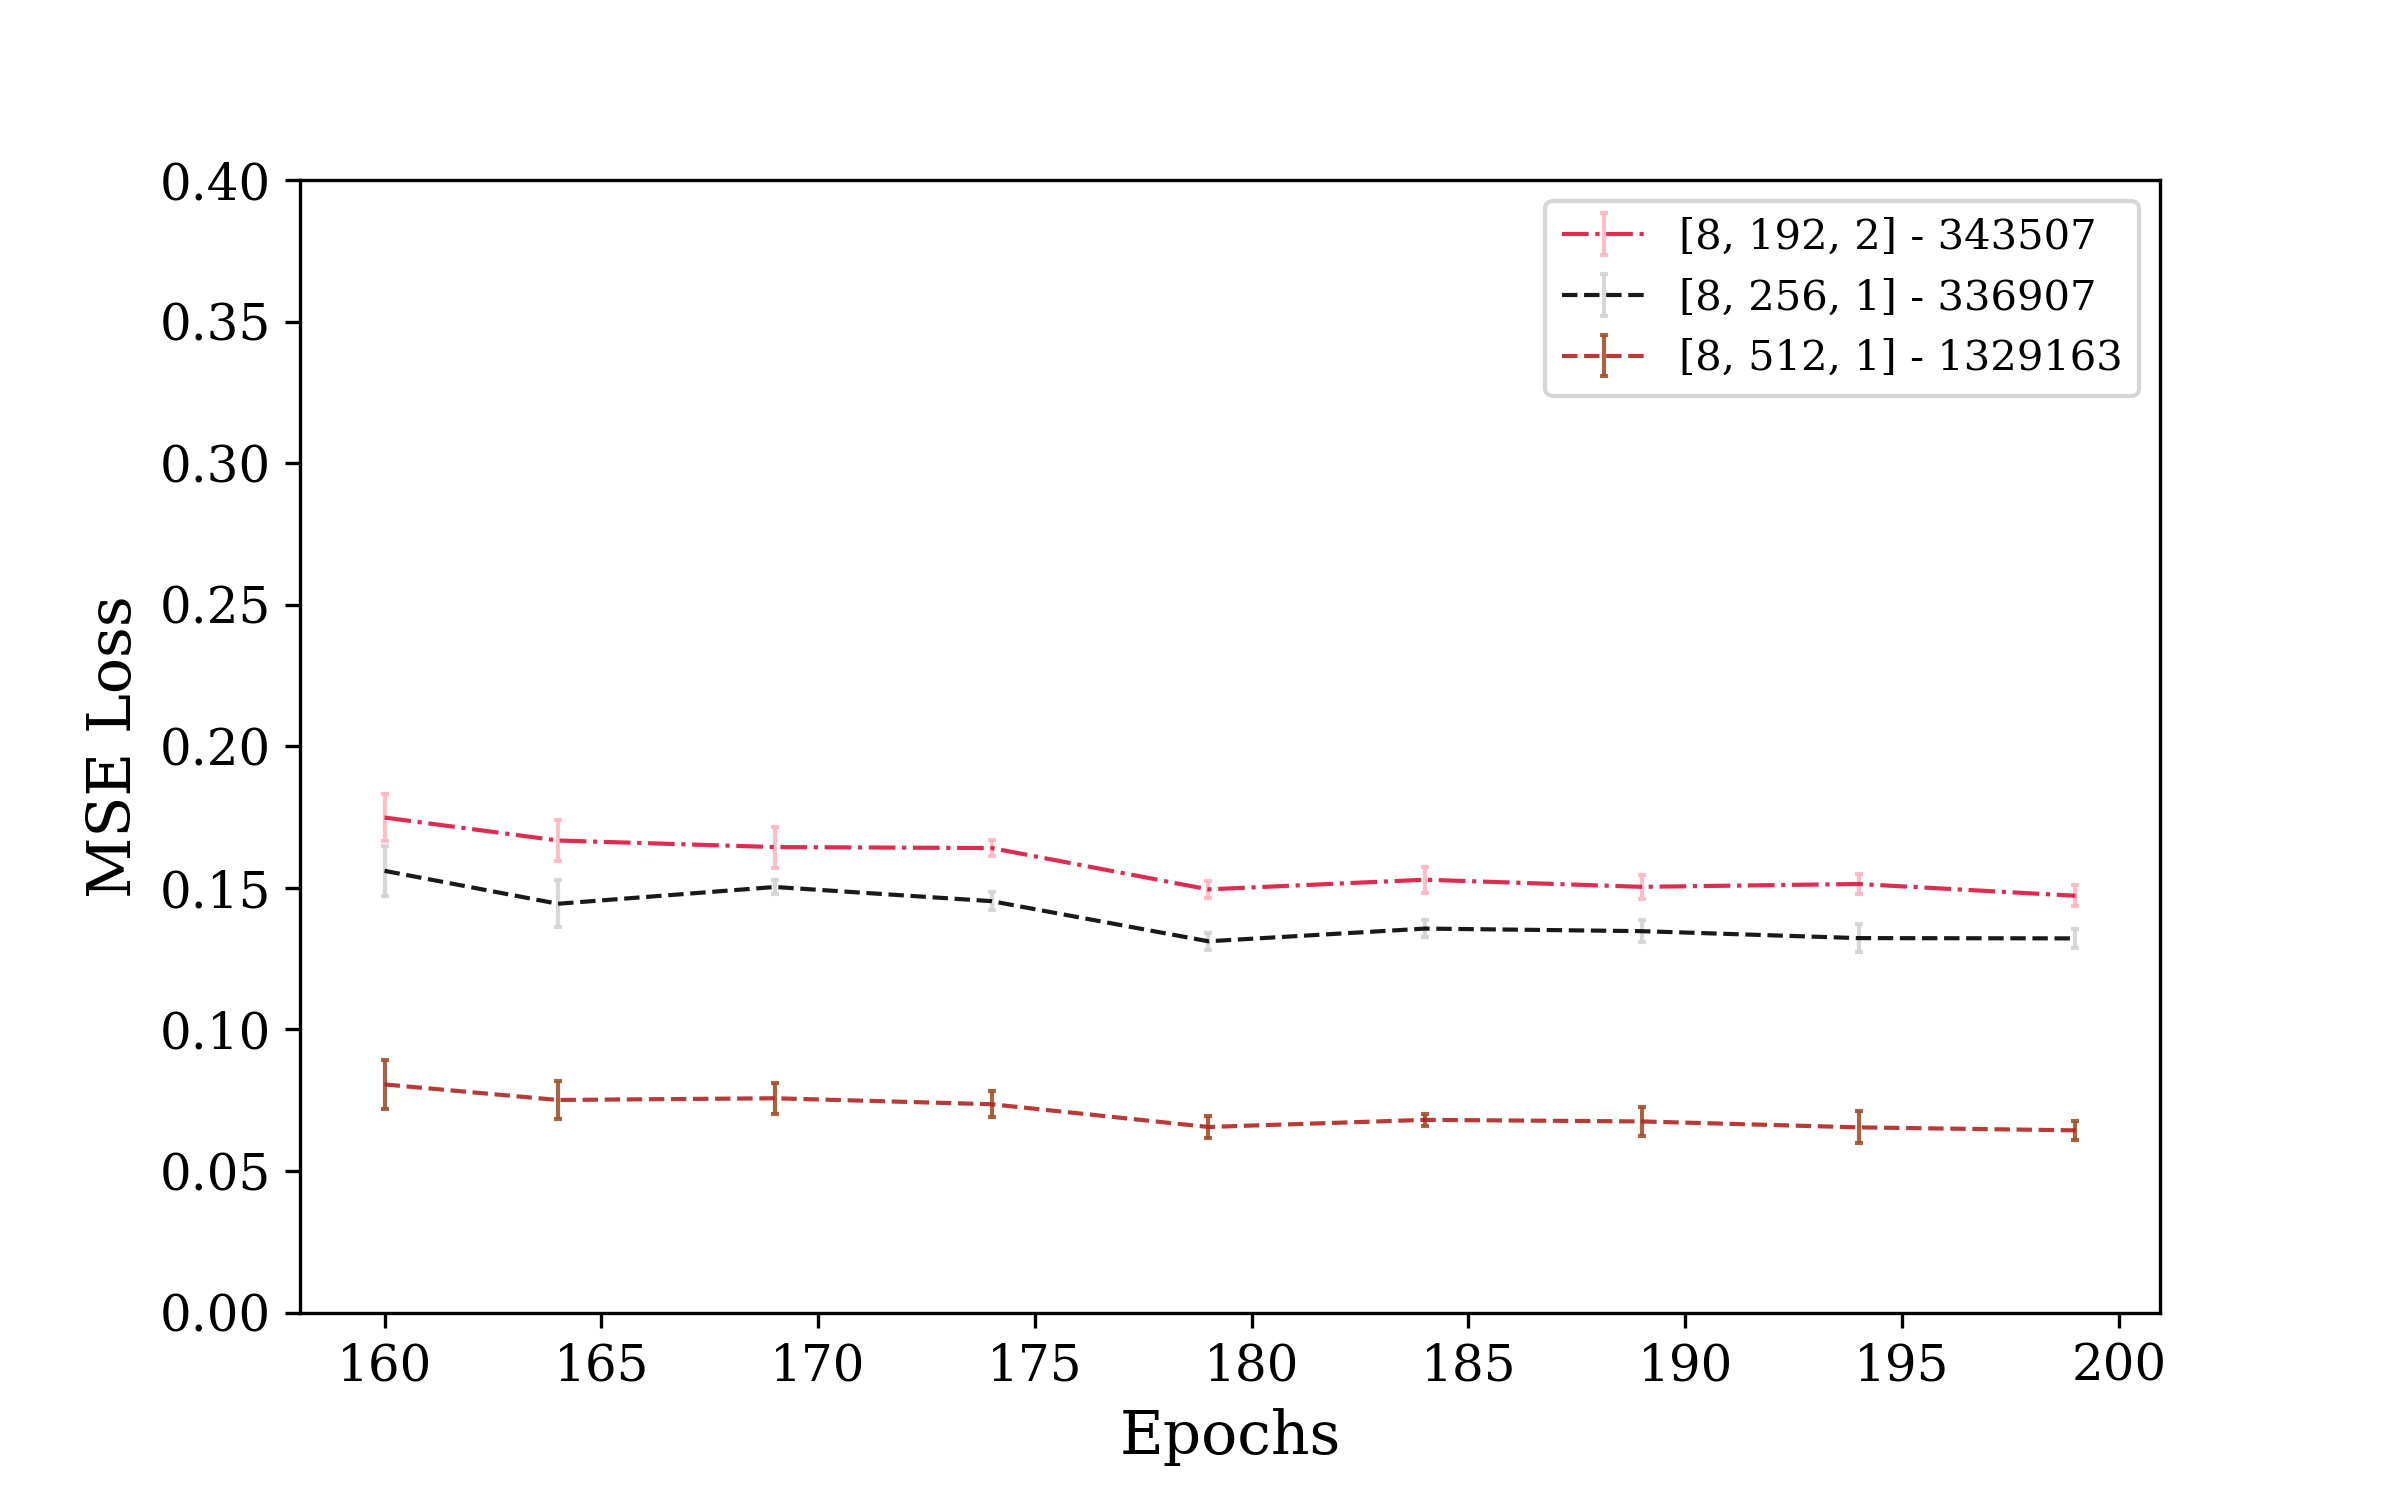
\includegraphics[width=15cm, keepaspectratio]{images/results/module_scalability_2.png}
                \caption{MSE Loss Function $L_{pred}$ of the trained modules between Epoch 160 and Epoch 200 for a better illustration. The right-hand side number in the legend is the total number of parameter of each module.}
                \label{fig:results_scalability_2}
        \end{figure}
        
        \begin{figure}[hbtp]
                \centering
                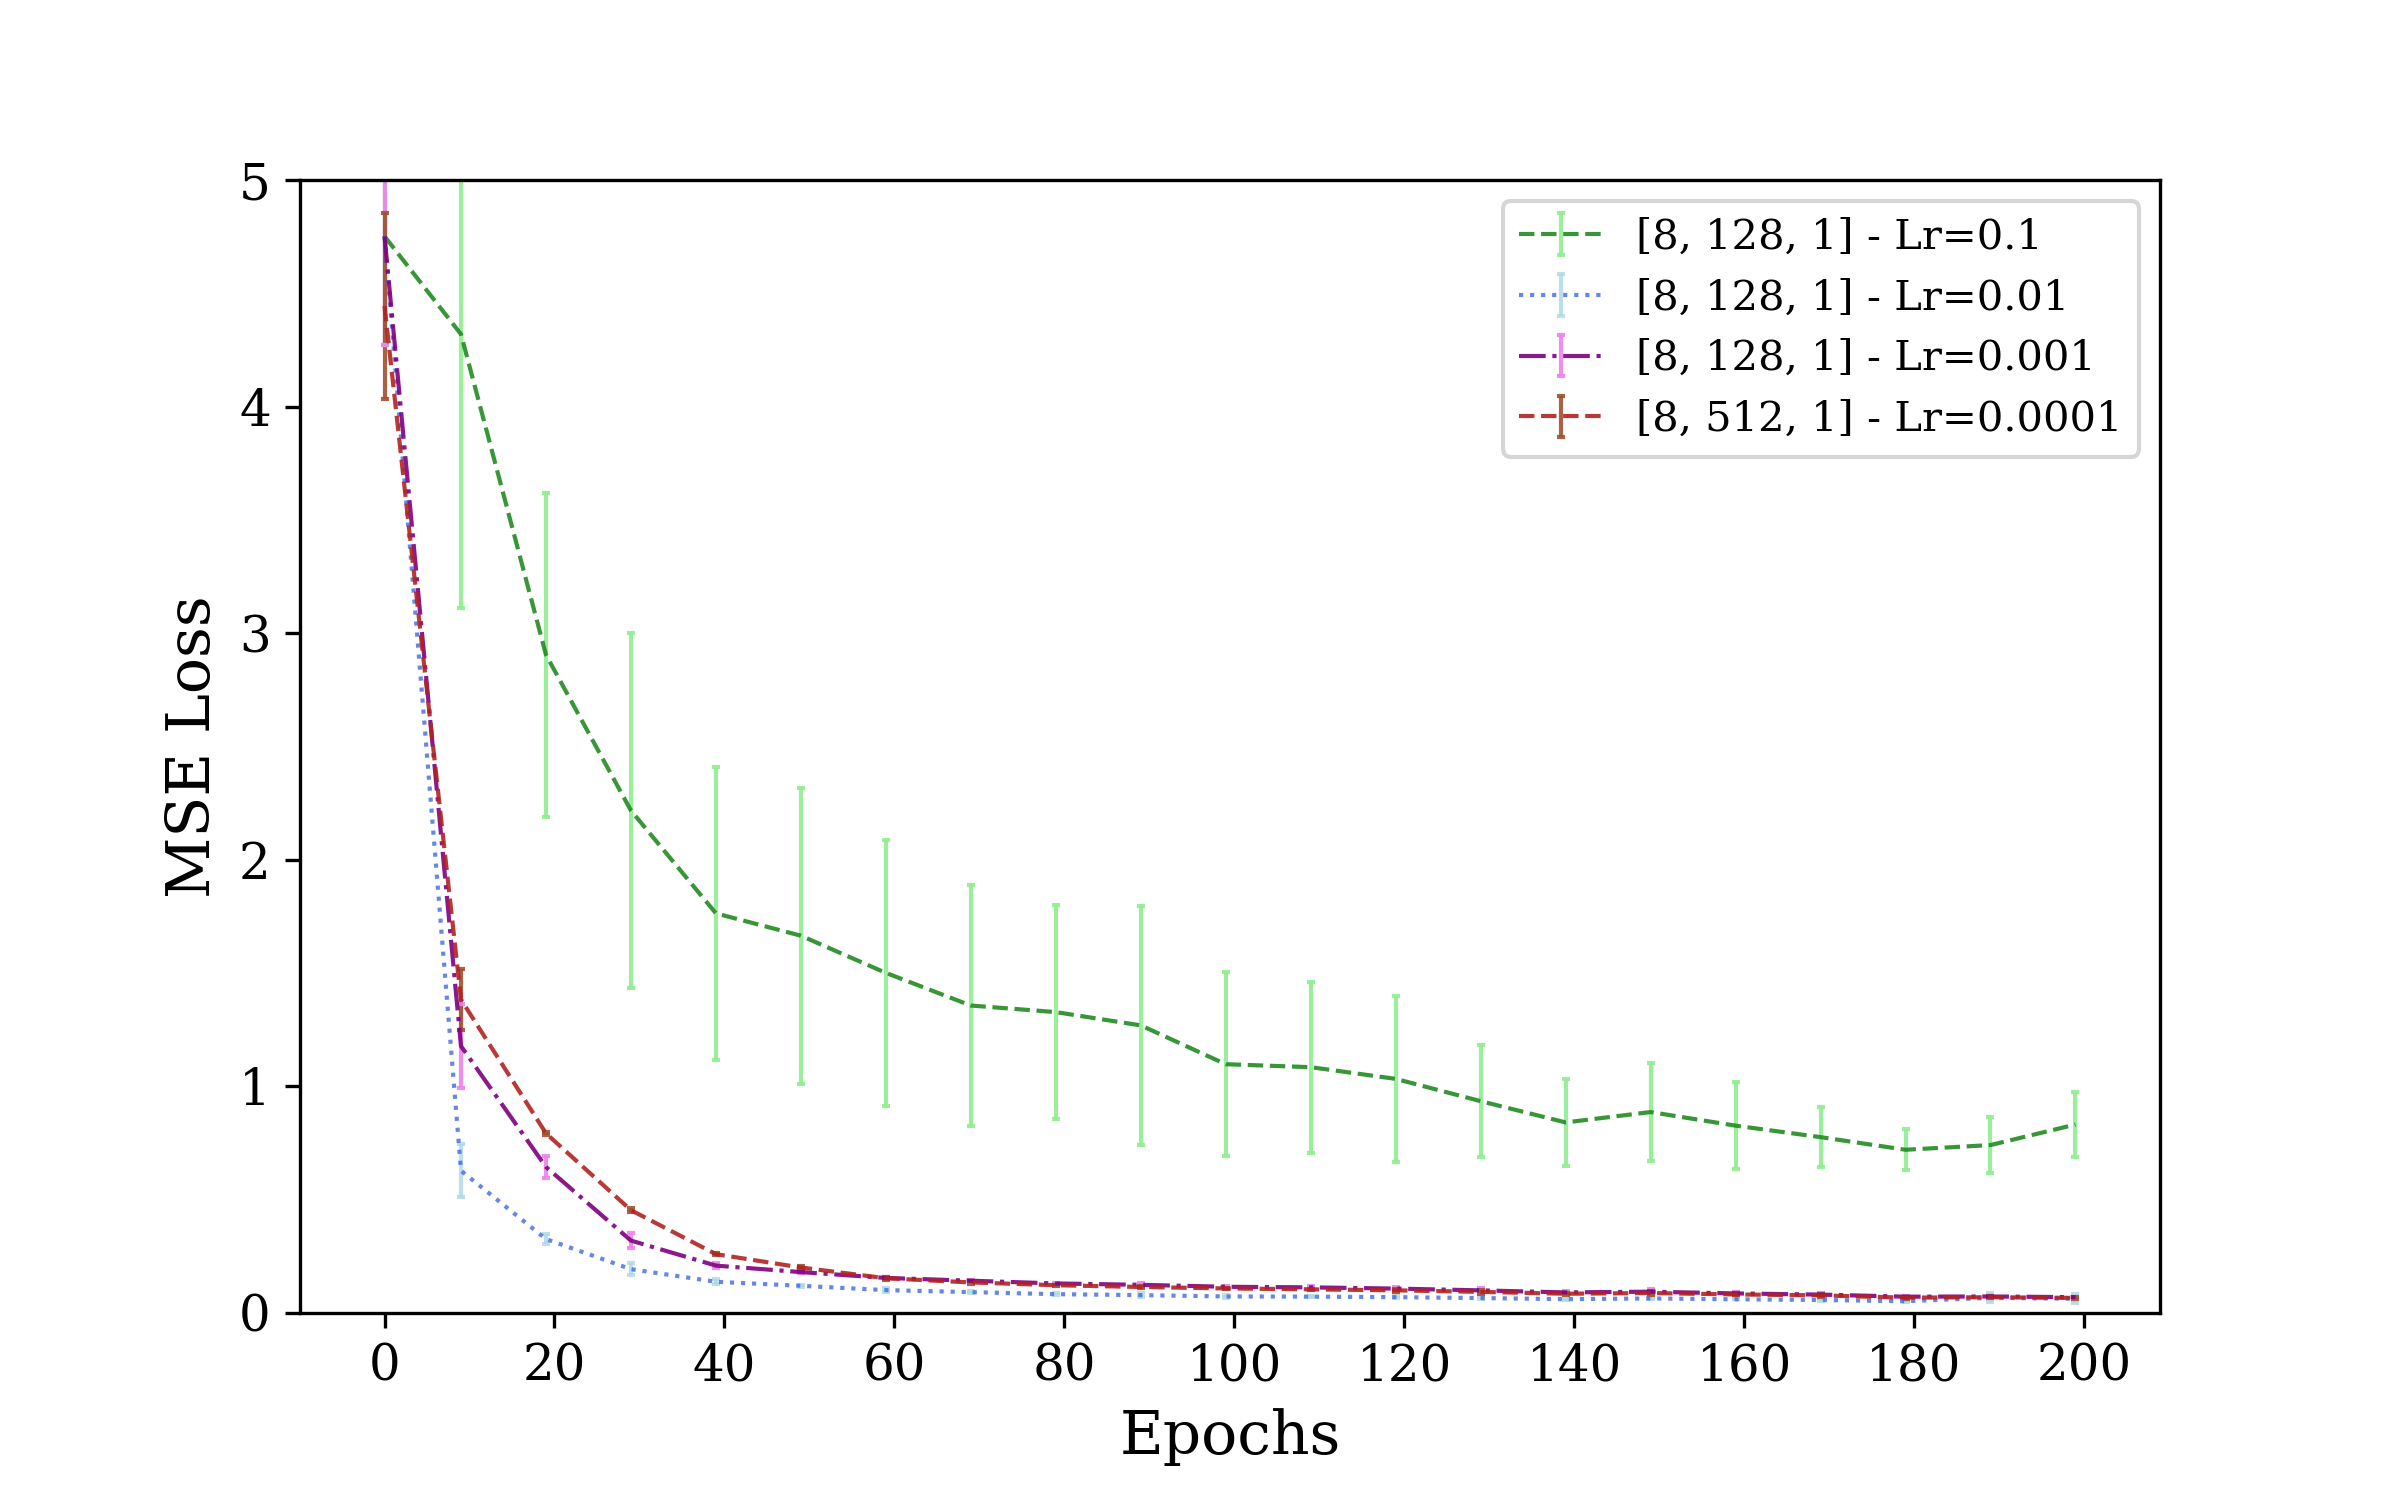
\includegraphics[width=15cm, keepaspectratio]{images/results/module_lr_2.png}
                \caption{MSE Loss Function $L_{pred}$ of the trained modules. The right-hand side number in the legend is the ADAM Learning Rate used for training.}
                \label{fig:results_lr_2}
                
                \vspace{1.5cm}
                
                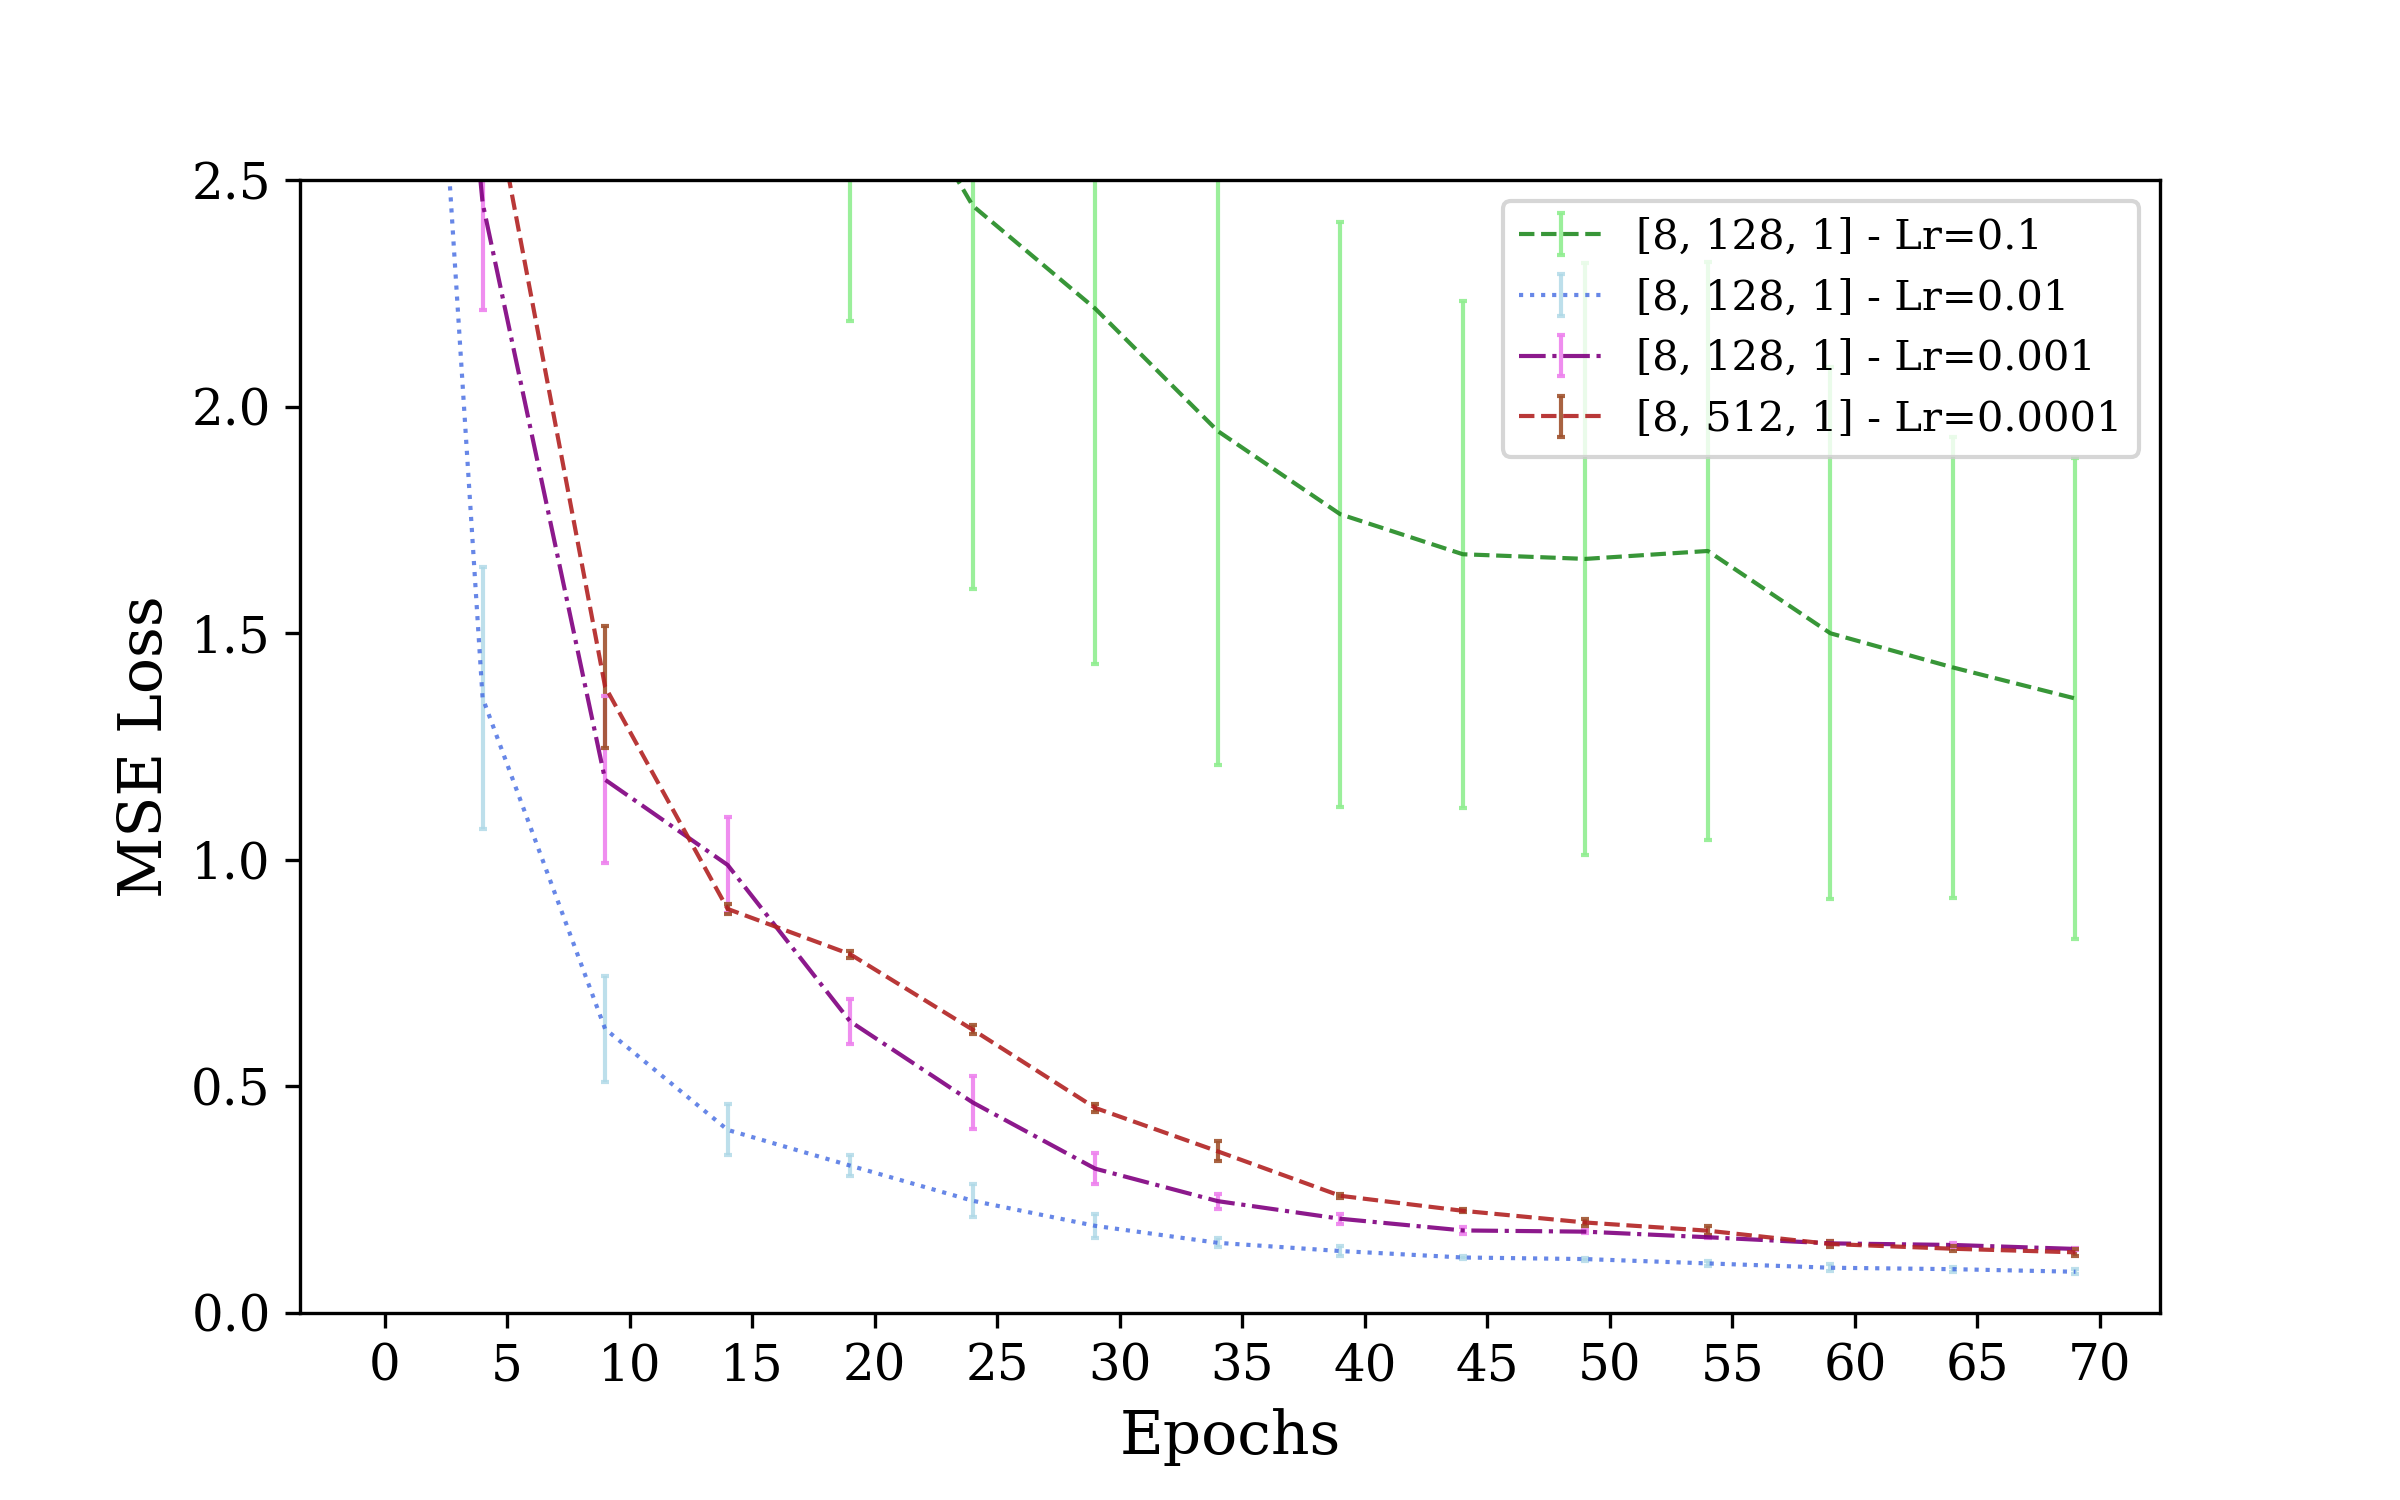
\includegraphics[width=15cm, keepaspectratio]{images/results/module_lr_1.png}
                \caption{MSE Loss Function $L_{pred}$ of the trained modules between Epoch 0 and Epoch 70 for a better illustration. The right-hand side number in the legend is the ADAM Learning Rate used for training.}
                \label{fig:results_lr_1}
        \end{figure}
        
        \begin{figure}[hbtp]
            \centering
            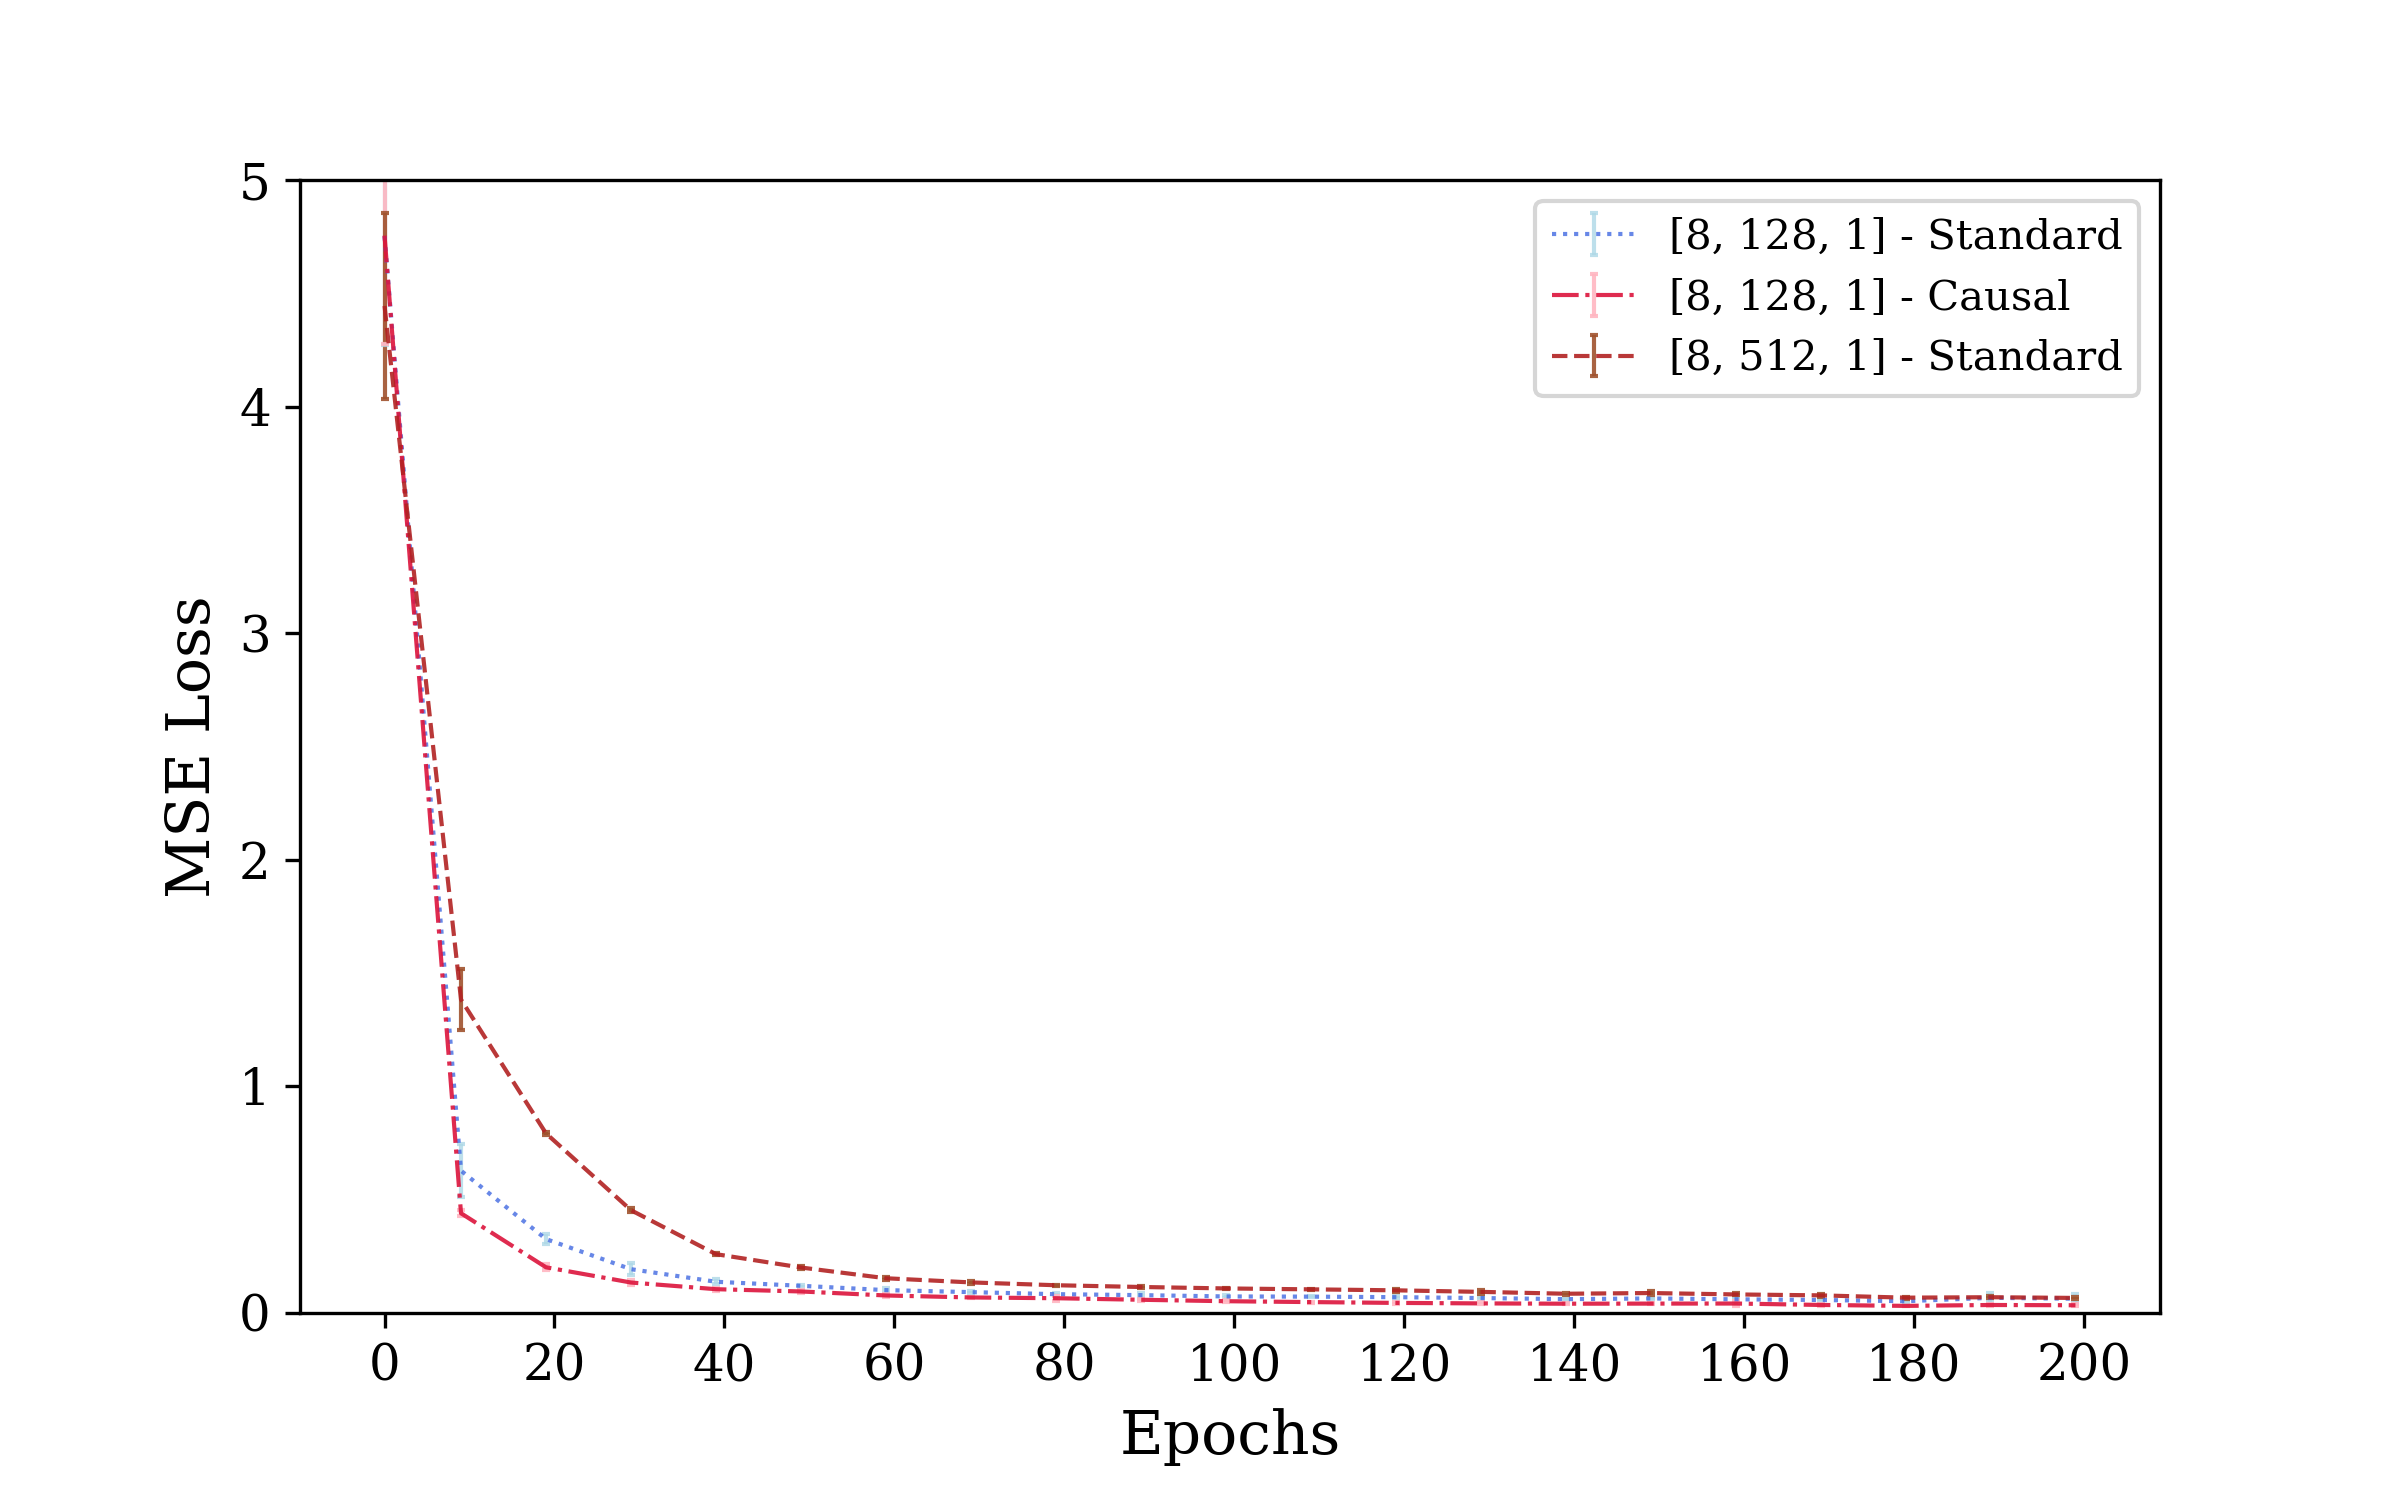
\includegraphics[width=15cm, keepaspectratio]{images/results/module_causal_1.png}
            \caption{MSE Loss Function $L_{pred}$ of the trained modules.}
            \label{fig:results_causal_1}
            
            \vspace{1.5cm}
            
            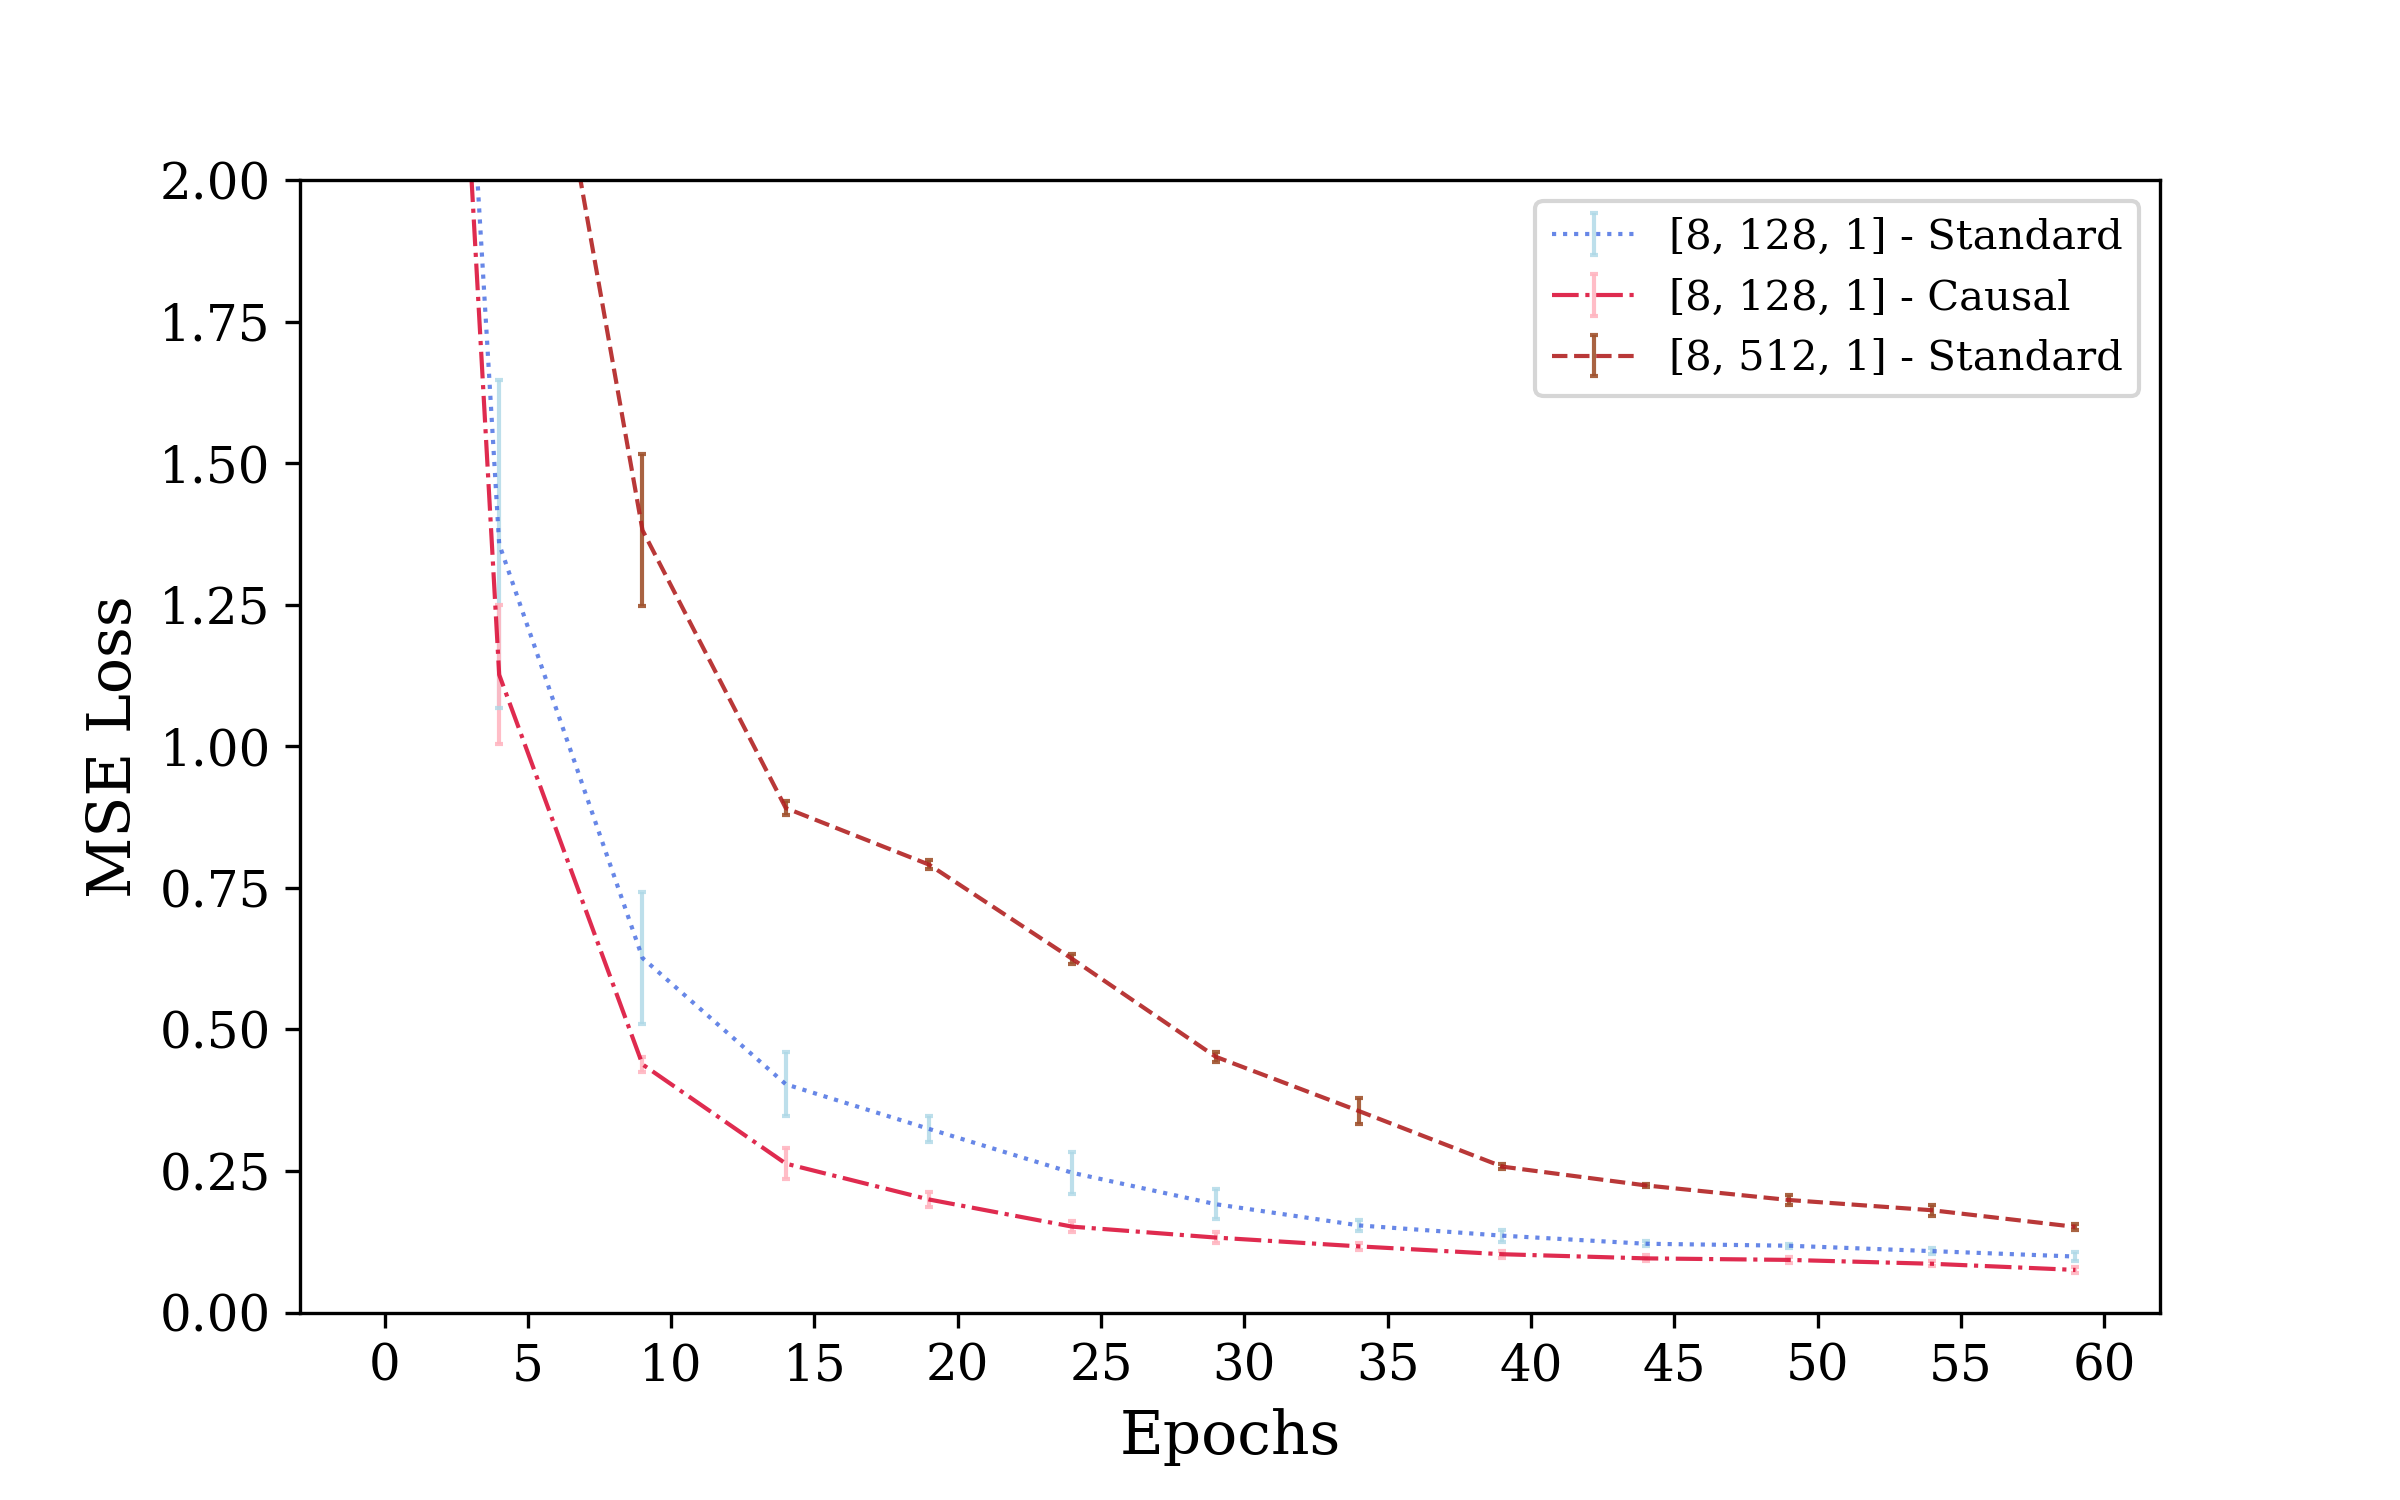
\includegraphics[width=15cm, keepaspectratio]{images/results/module_causal_2.png}
            \caption{MSE Loss Function $L_{pred}$ of the trained modules between Epoch 0 and Epoch 60 for a better illustration.}
            \label{fig:results_causal_2}
        \end{figure}
        
    \newpage
    \section{Deterministic Environment}
    \label{results:deterministic}
    % Inverted Pendulum Results
        This Section is dedicated to results obtained in the deterministic environment Inverted Pendulum. It is divided in two sub-sections: Section \ref{sub:res_det_delays} is concerned with training results obtained by simulated different amount of deterministic and constant delay, while Section \ref{sub:res_stoch_delays} presents training results obtain by simulating the presence of stochastic delays by means of the stochastic process described in Section \ref{sub:simulated_delays}. At the end, the last Section \ref{sub:res_test_delays} discusses the capabilities of the original approach when tested on environments in which the amount of simulated delay is different w.r.t. the one they were trained with. 
        
        \subsection{Deterministic Delays Training Results}
        \label{sub:res_det_delays}
            % SARSA, DSARSA, A-TRPO, M-TRPO, L2-TRPO and D-TRPO Comparison
            All baselines described in Section \ref{sub:baselines}, L2-TRPO and D-TRPO have been trained in the Inverted Pendulum environment. In particular, A-TRPO, M-TRPO and D-TRPO are equipped with policy networks composed of 2 feedforward layers of 64 neurons each and with value function networks composed of 1 feedforward layer of 64 neurons. L2-TRPO has been trained with a policy network composed of 2 feedforward layer of 67 neurons each and with a value function network with 1 feedforward layer of 128 neurons. D-TRPO and L2-TRPO have been deployed respectively with a [8, 64, 1] and a [8, 68, 1] modules, according to the notation presented in Section \ref{results:module_tuning}. L2-TRPO parameters have been slightly enlarged so that the entire network has a similar total number of parameters to D-TRPO, which is also equipped with a MAF network. All algorithms have been trained for 2000 epochs, each composed of 5000 steps for a total of 10 millions steps. Each trajectory in the environment lasts for 250 steps. Each algorithm has been trained with different amounts of deterministic and costant simulated delay, specifically we chose to test 3, 5, 10 and 15 time-steps of delay. At last, TRPO has beed trained on the same context without delays as a reference for the best possible performance it is possible to obtain.
            
            \subsubsection{Results Description}
                We start discussing the results from the 3-steps delay and then increasing delay. As figure \ref{fig:results_delay3_1} shows, D-TRPO, L2-TRPO and M-TRPO are able to cope with 3 steps of delay without particular issues: while M-TRPO is slightly slower than the other two, they are able to reach undelayed TRPO's average reward, albeit slower. Instead, A-TRPO is already greatly affected by the state augmentation and it does not manage to converge towards the optimal behaviour. At the same time, both SARSA and D-SARSA converge to a slightly better performance than A-TRPO, while still being substantially affected by the delay.\newline
                Training with 5 steps of delays shows similar results: as expected, each algorithm is affected by the larger delay with slower convergence and/or slower final average reward. The main observable difference is the loss of performances that M-TRPO shows, without being able to reach the same level of performances of undelayed TRPO.\newline
                A delay of 10 time-step heavily affects even L2-TRPO and D-TRPO, which are still able to outperform the other algorithms, but they no longer match undelayed TRPO performances. At the end, 15 steps of delay proves to be too large for any algorithm to show a significant performance improvement, with M-TRPO reaching the best result overall.
            
            \subsubsection{Result Discussion}
                This set of training procedures shows that the proposed approach is solid and able to produce promising results. Both D-TRPO and L2-TRPO are able to outperform almost any other baselines, regardless the amount of delay present, even matching undelayed TRPO performances for lower delays, effectivaly nullfying the presence of delays. However, it is also interesting to note that M-TRPO is also able to keep up throughout the tests and it proves to be more resilient that other algorithms to large delays, possibly suggesting that it could be the preferred method in some range of delays. 
            
            \begin{figure}[hbtp]
                \centering
                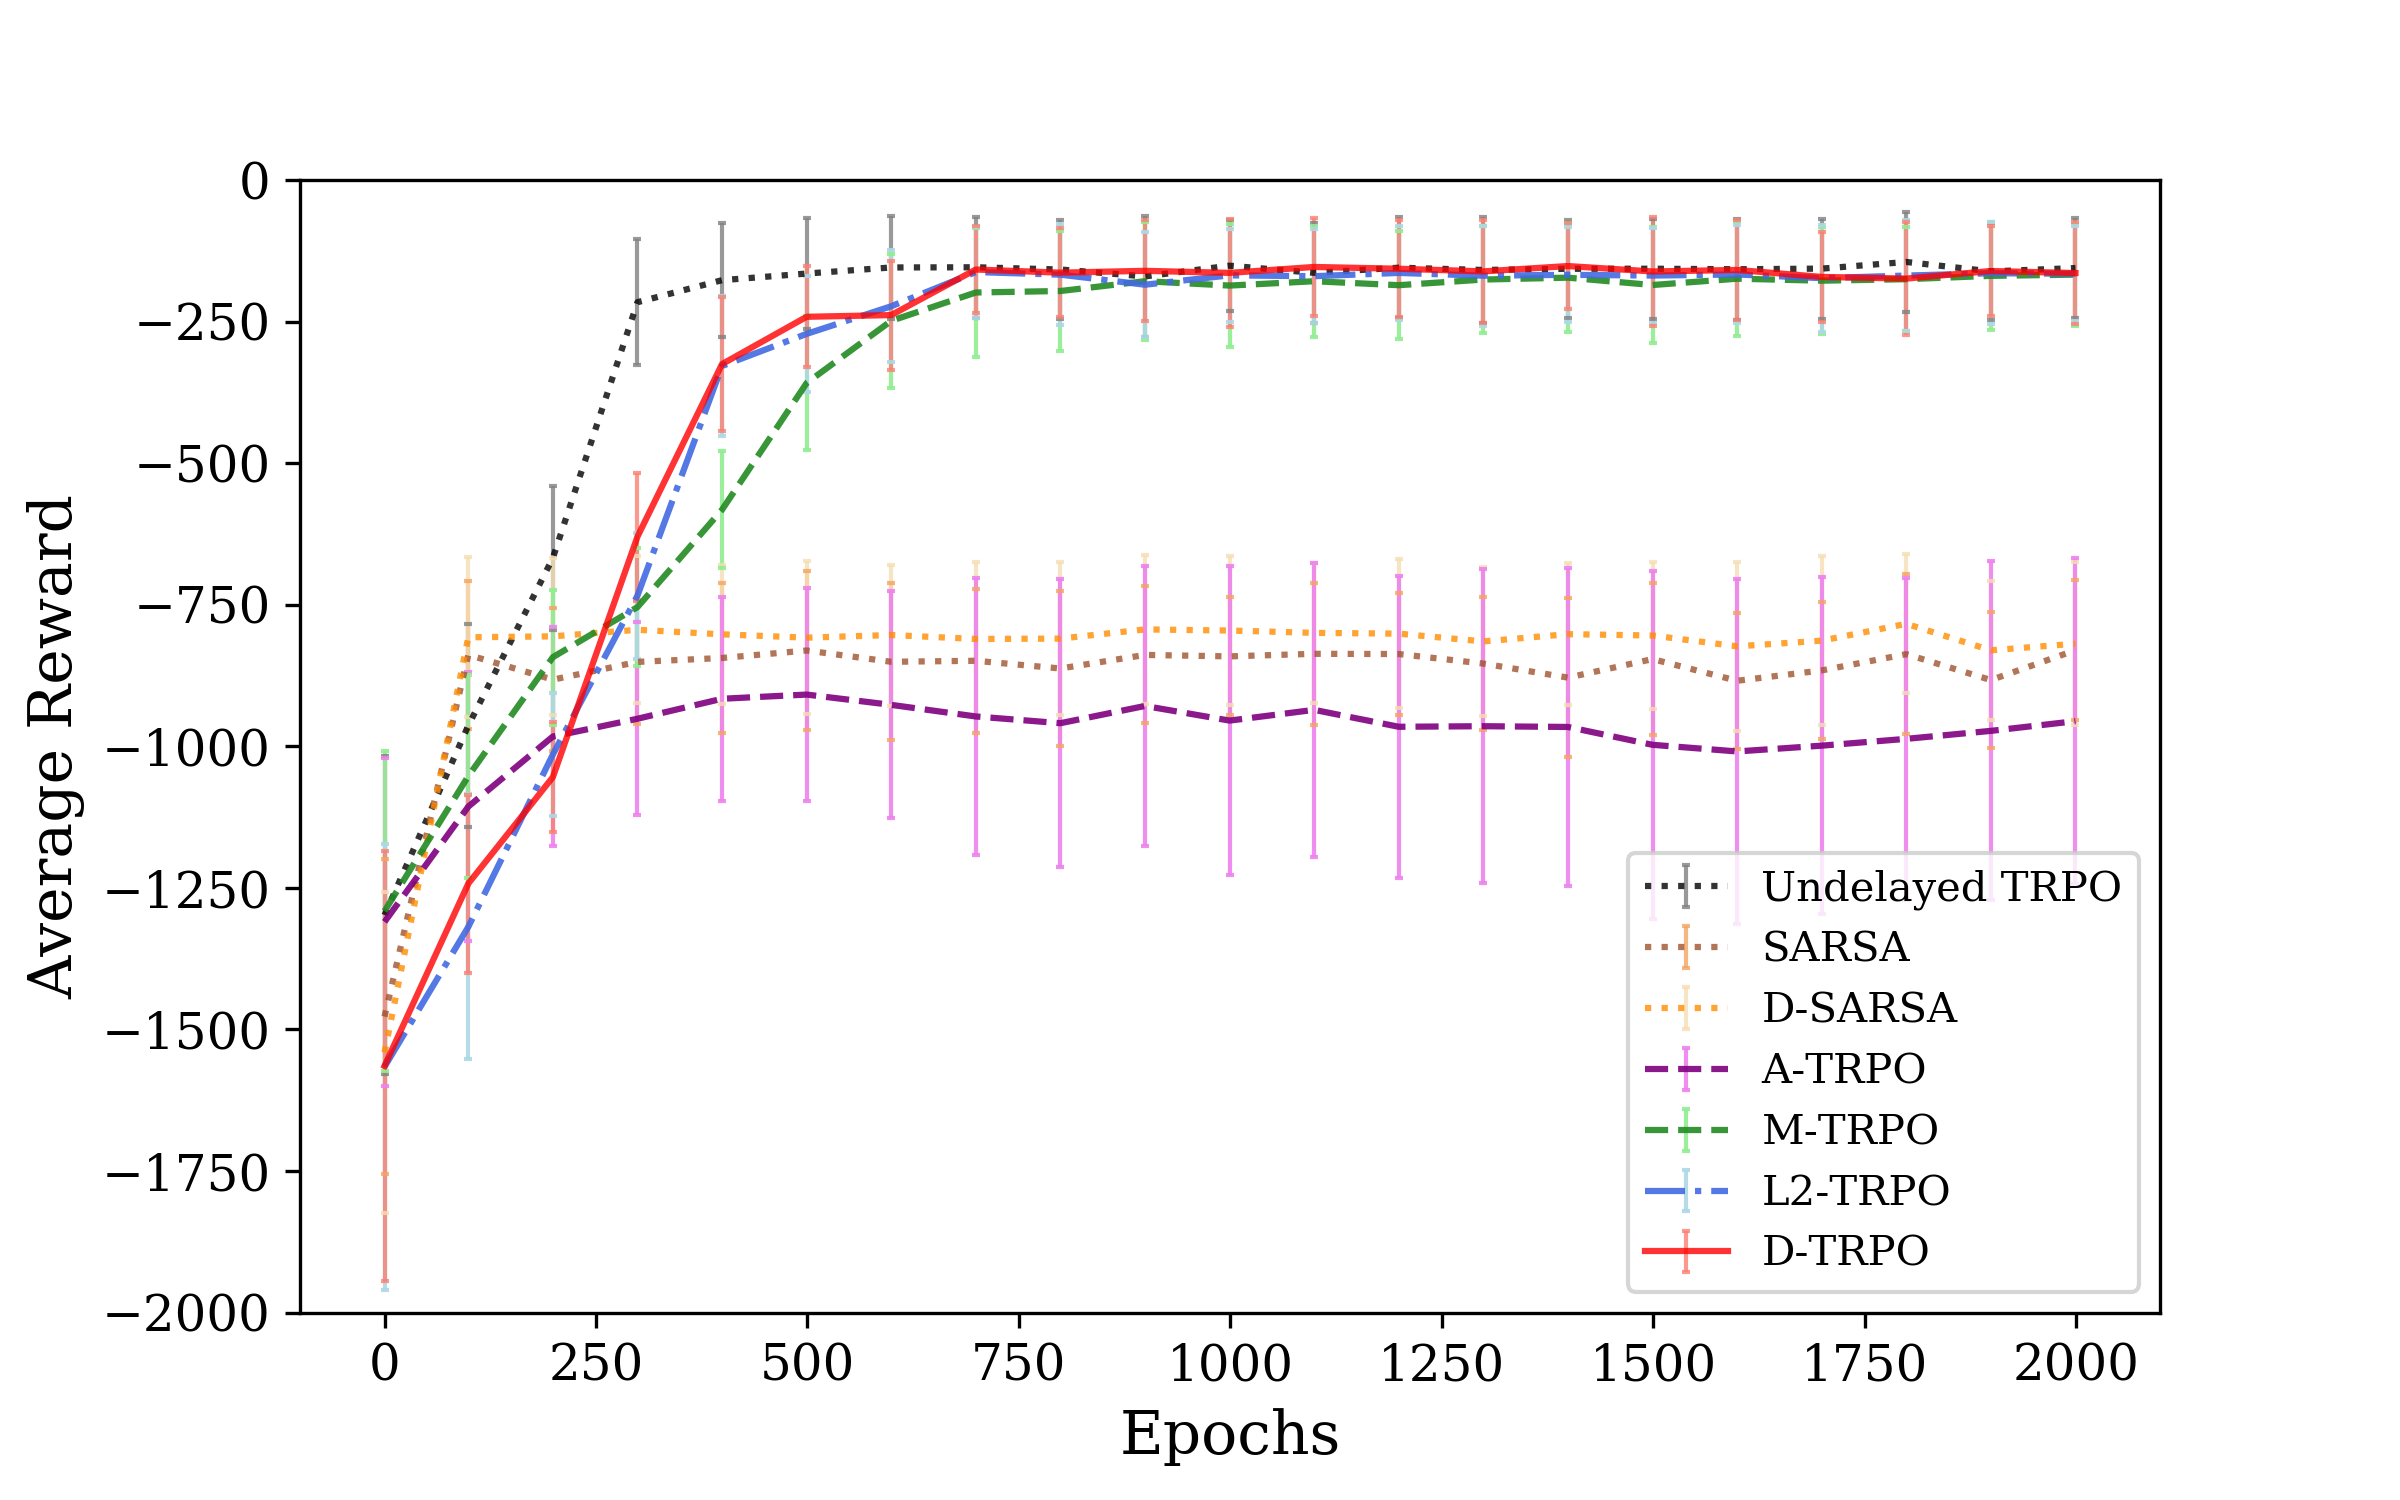
\includegraphics[width=15cm, keepaspectratio]{images/results/delay3_comparisons_1.png}
                \caption{Training results obtained in a 3-steps delay and deterministic environment setting.}
                \label{fig:results_delay3_1}
                
                \vspace{1.5cm}
                
                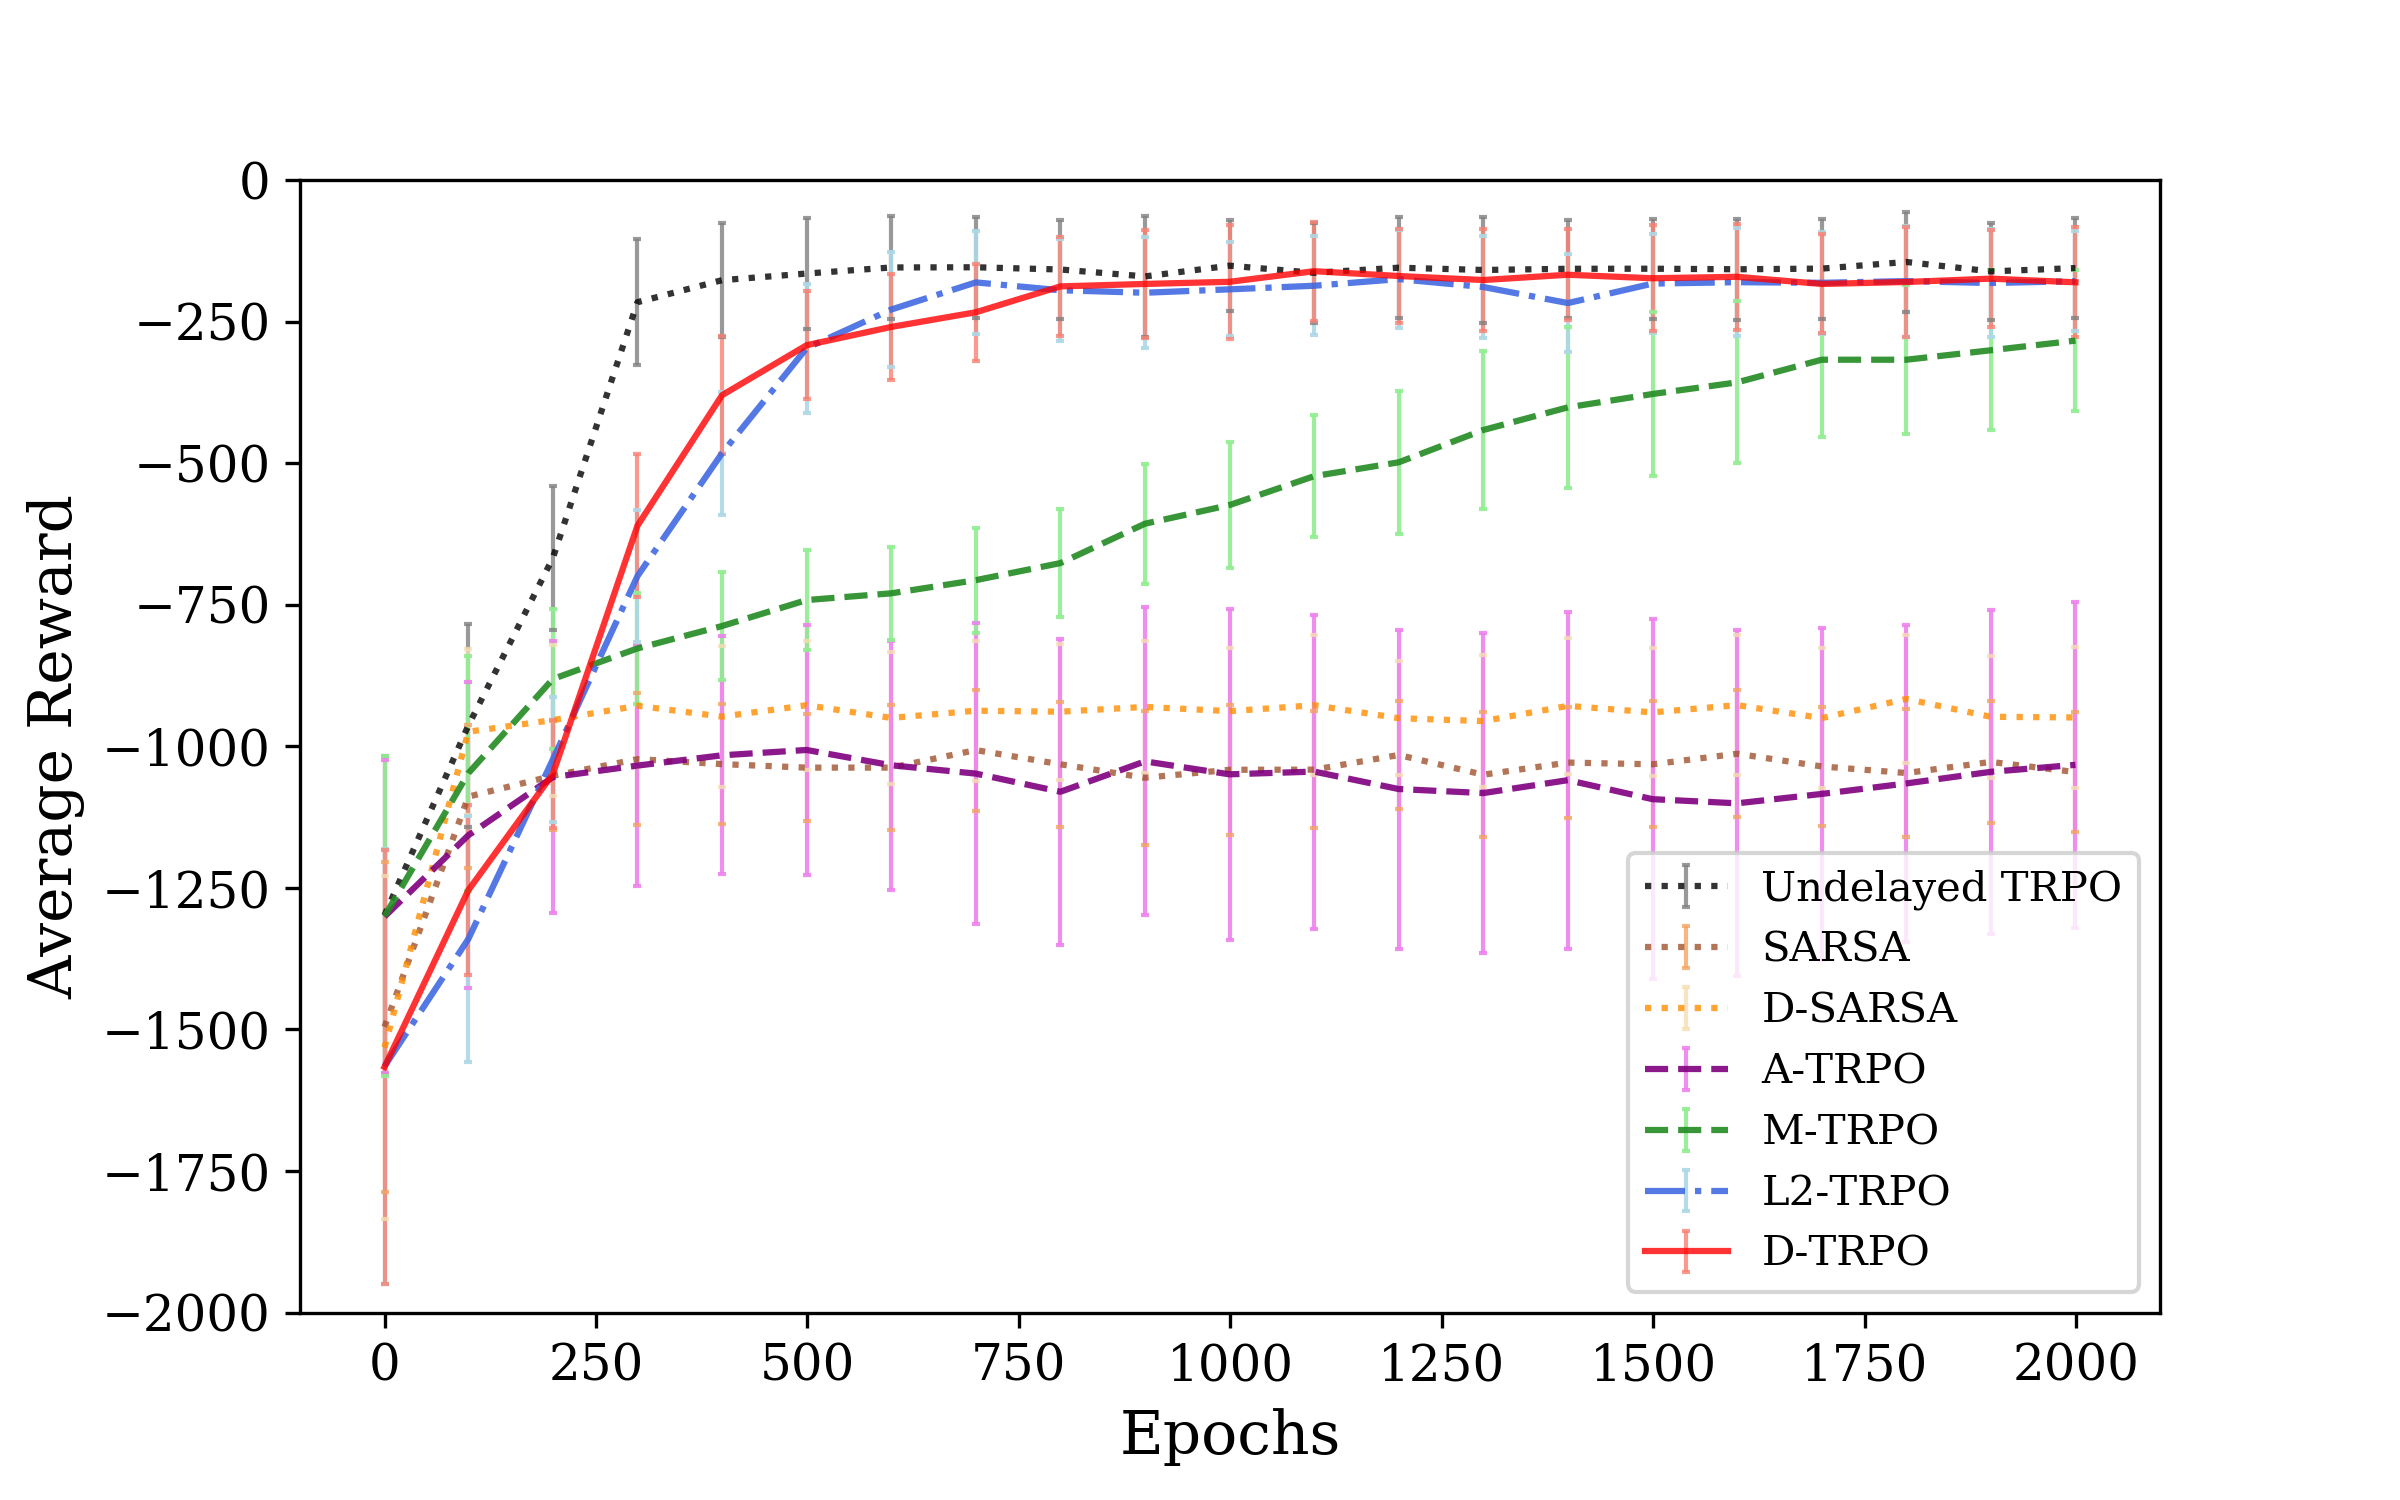
\includegraphics[width=15cm, keepaspectratio]{images/results/delay5_comparisons_1.png}
                \caption{Training results obtained in a 5-steps delay and deterministic environment setting.}
                \label{fig:results_delay5_1}
            \end{figure}
            
            \begin{figure}[hbtp]
                \centering
                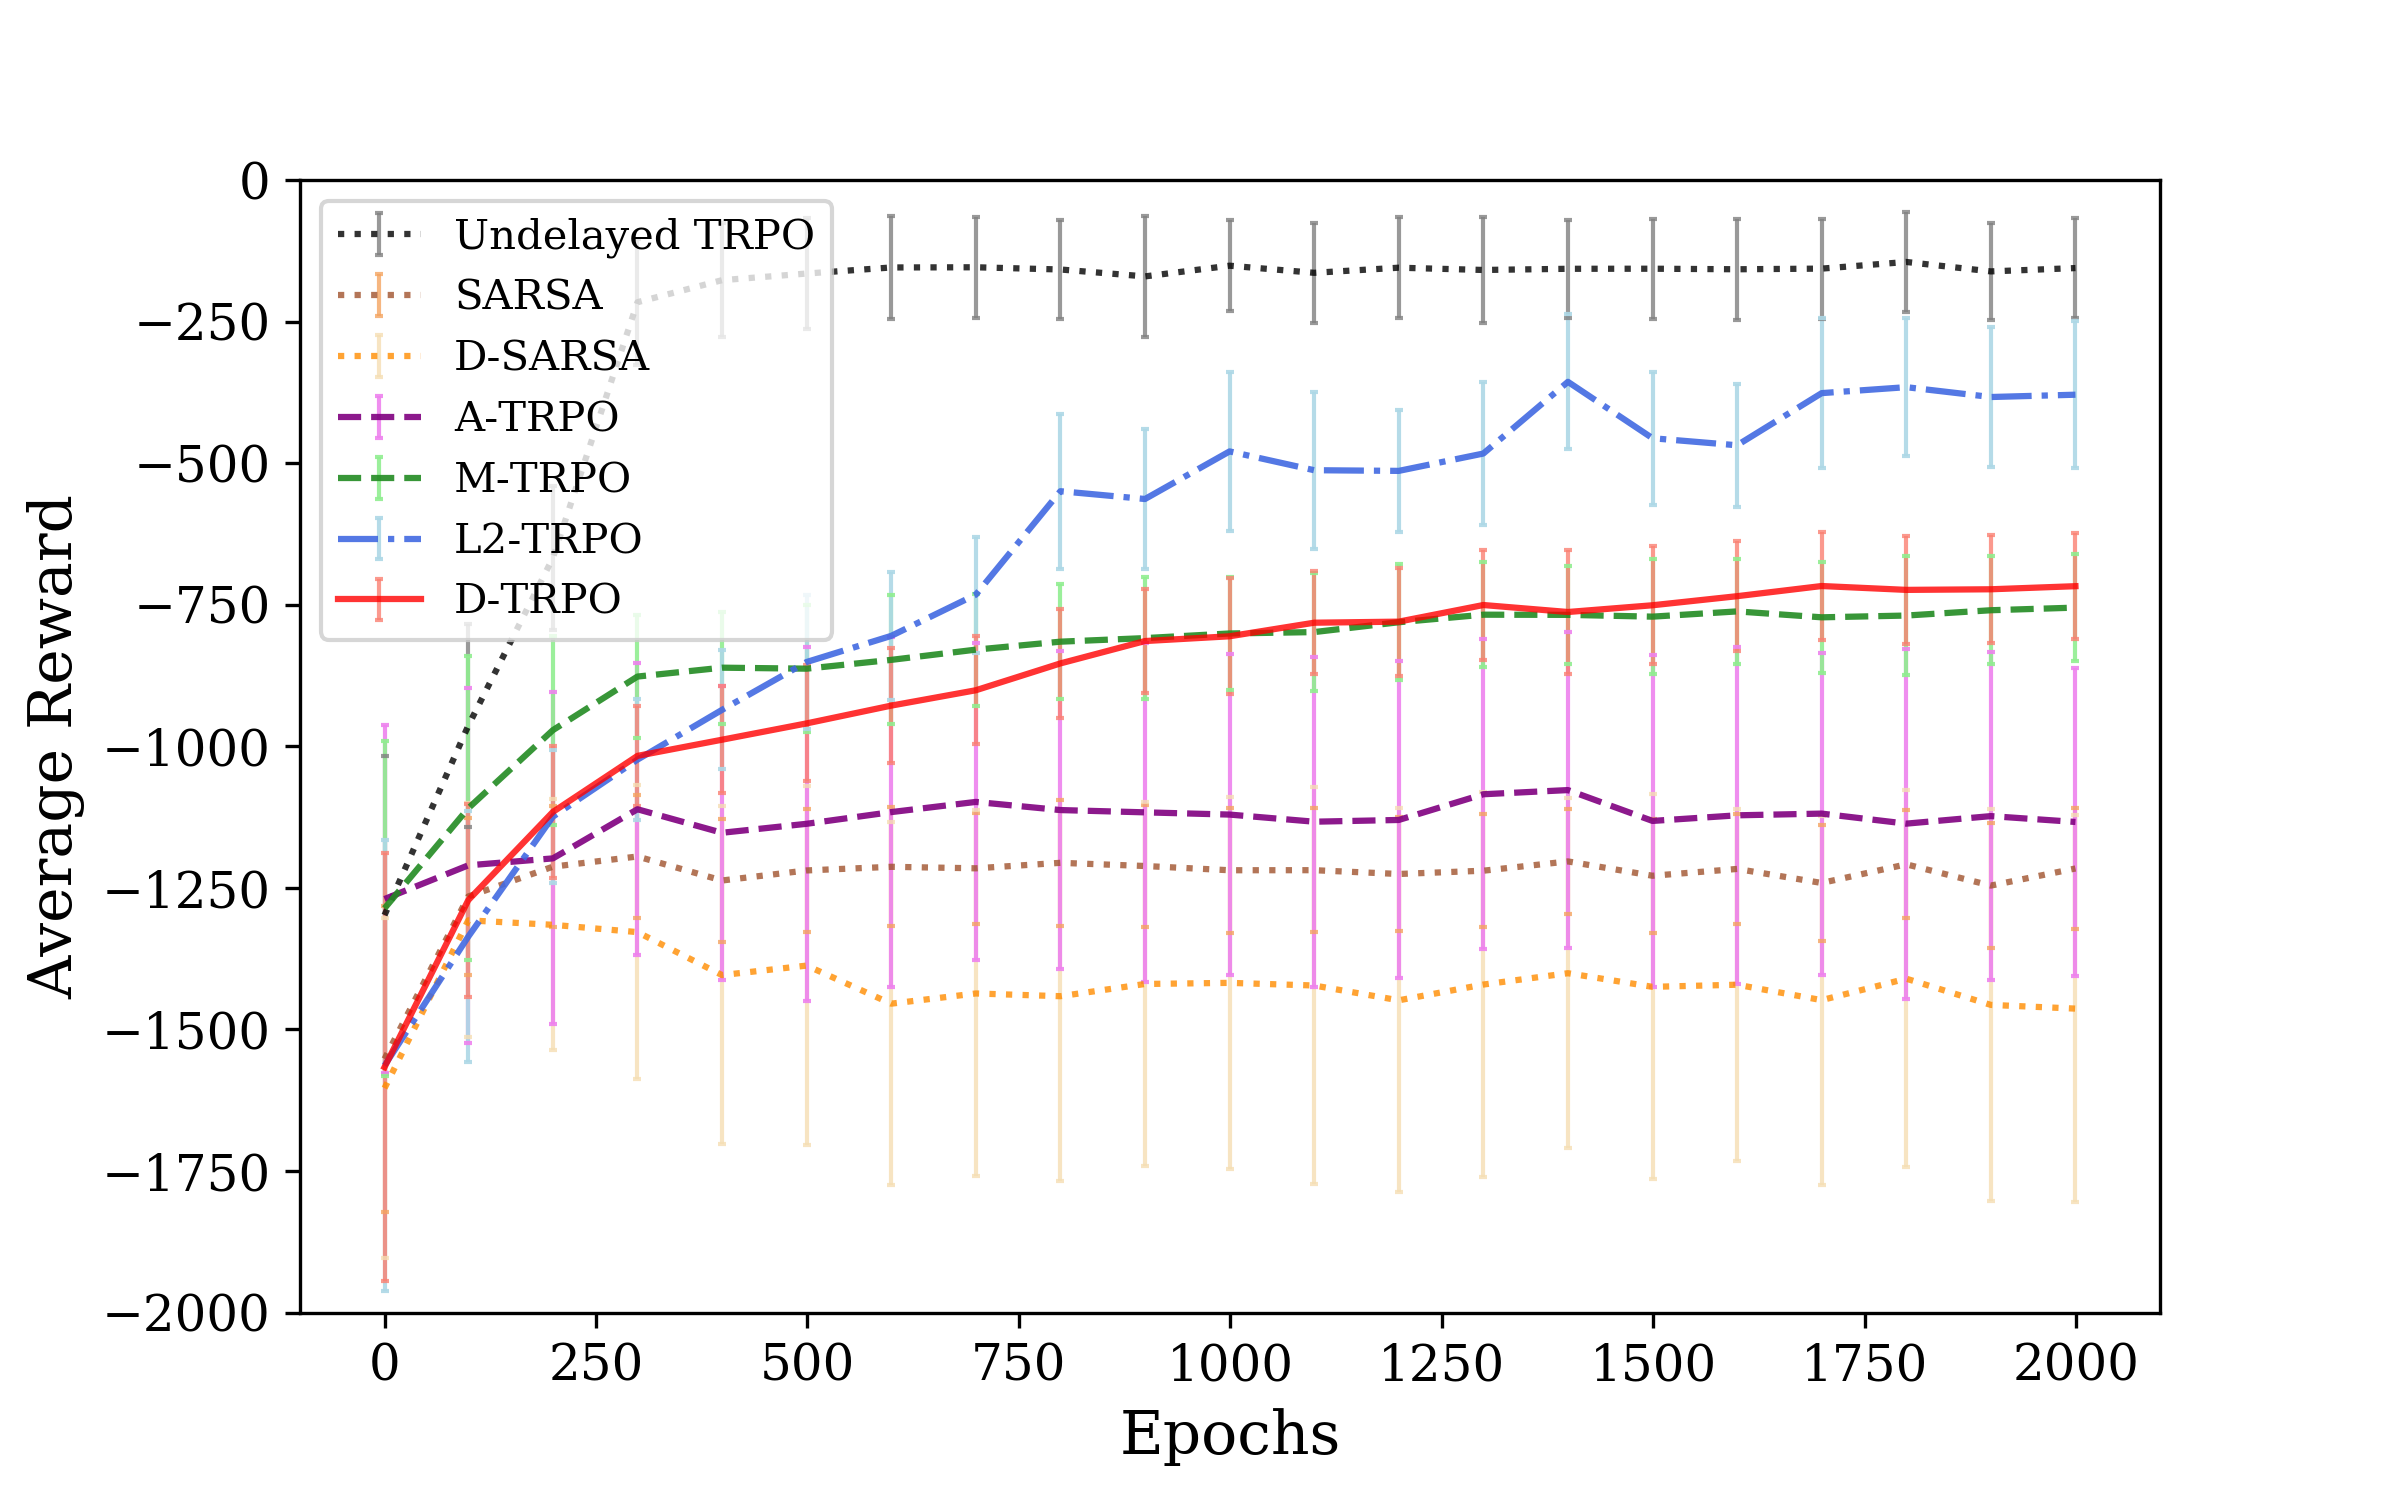
\includegraphics[width=15cm, keepaspectratio]{images/results/delay10_comparisons_1.png}
                \caption{Training results obtained in a 10-steps delay and deterministic environment setting.}
                \label{fig:results_delay10_1}
                
                \vspace{1.5cm}
                
                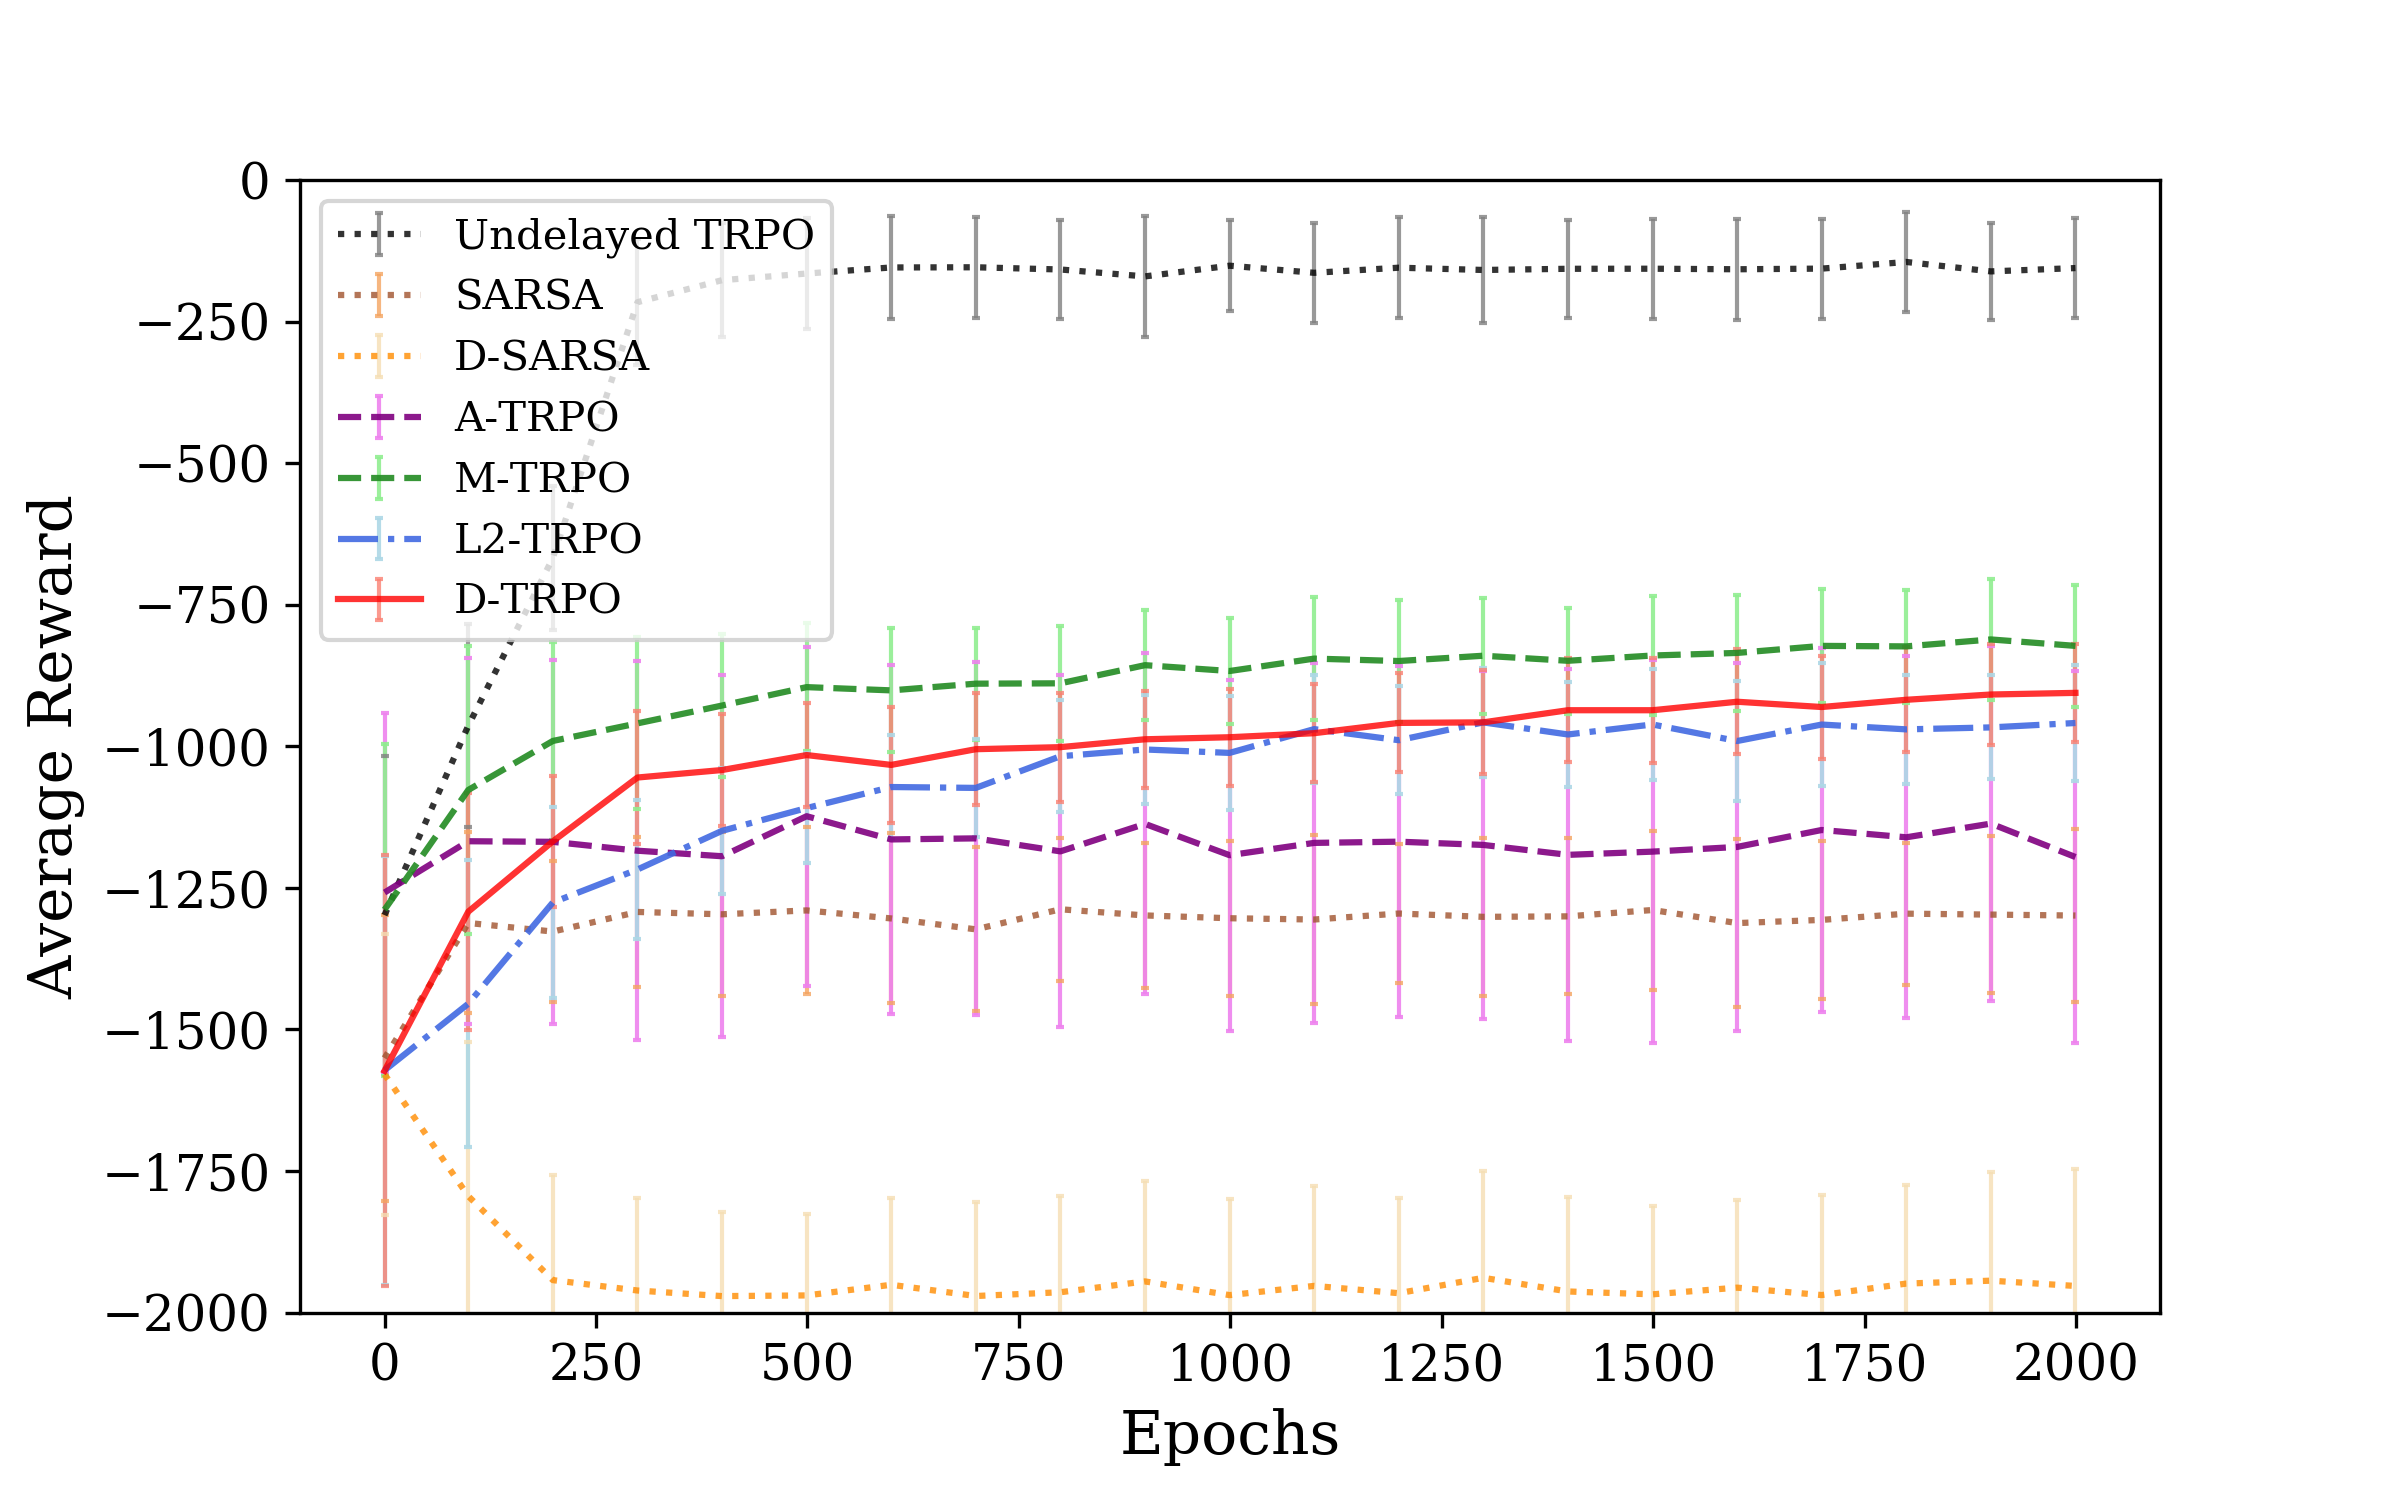
\includegraphics[width=15cm, keepaspectratio]{images/results/delay15_comparisons_1.png}
                \caption{Training results obtained in a 15-steps delay and deterministic environment setting.}
                \label{fig:results_delay15_1}
            \end{figure}
        
        \newpage
        \subsection{Stochastic Delays Training Results}
        \label{sub:res_stoch_delays}
            % Only D-TRPO and L2-TRPO can natively handle them (Attention Network)
            % D-TRPO Tests --> Bad Results, keep training on Deterministic
            % Compare the trained model on Stochastic Delays against the Min/Max Deterministic Delay
            We decided to test D-TRPO in a stochastic delay context, deploying the same settings for the networks as in the previous test. We train D-TRPO for 500 epochs composed of 5000 steps each, while each trajectory in the environment lasts for 250 steps, and simulating three different stochastic delay processes respectively with $p=0.7$, $p=0.6$ and $p=0.55$.
            \\\\
            Figures \ref{fig:results_delayp07_1}, \ref{fig:results_delayp06_1} and \ref{fig:results_delayp05_1} illustrates the resulting training process, comparing them to D-TRPO and L2-TRPO trained with a constant delay closest to the average delay of each stochastic process, also shown in Figures \ref{fig:delayp07_sampledelay}, \ref{fig:delayp06_sampledelay} and \ref{fig:delayp05_sampledelay} respectively. Unfortunately, results are underwhelming compared with similar deterministic delays. Starting from $p=0.7$, which is compared to 3 steps of delays, D-TRPO shows an inconsistent learning process that converges to a lower average reward, even decreasing w.r.t. its peak performances. Stochastic delays with $p=0.6$ is compared to 5 steps of delays and they show similar results, while $p=0.5$ is compared with 10 steps of delay and shows very kin performances at 500 epochs, nevertheless D-TRPO with stochastic delays has already converged.
            The reason behind inconsistent performances may be related to the higher variance the stochastic delay process induces in the input data, the extended states. While in deterministic delays we expect the extended state to have a fixed size and, consequently, the module to predict the same number of steps at each time-step, stochastic delays disrupt this process: the extended state has a different size and the same set of parameter must be able to predict for a different number of time steps. Thus, the module needs to be able to deal not only with all possible combinations of states and sequence of actions in the extended state, but also with all possible sizes of the extended state. 
            
            \begin{figure}[!b]
                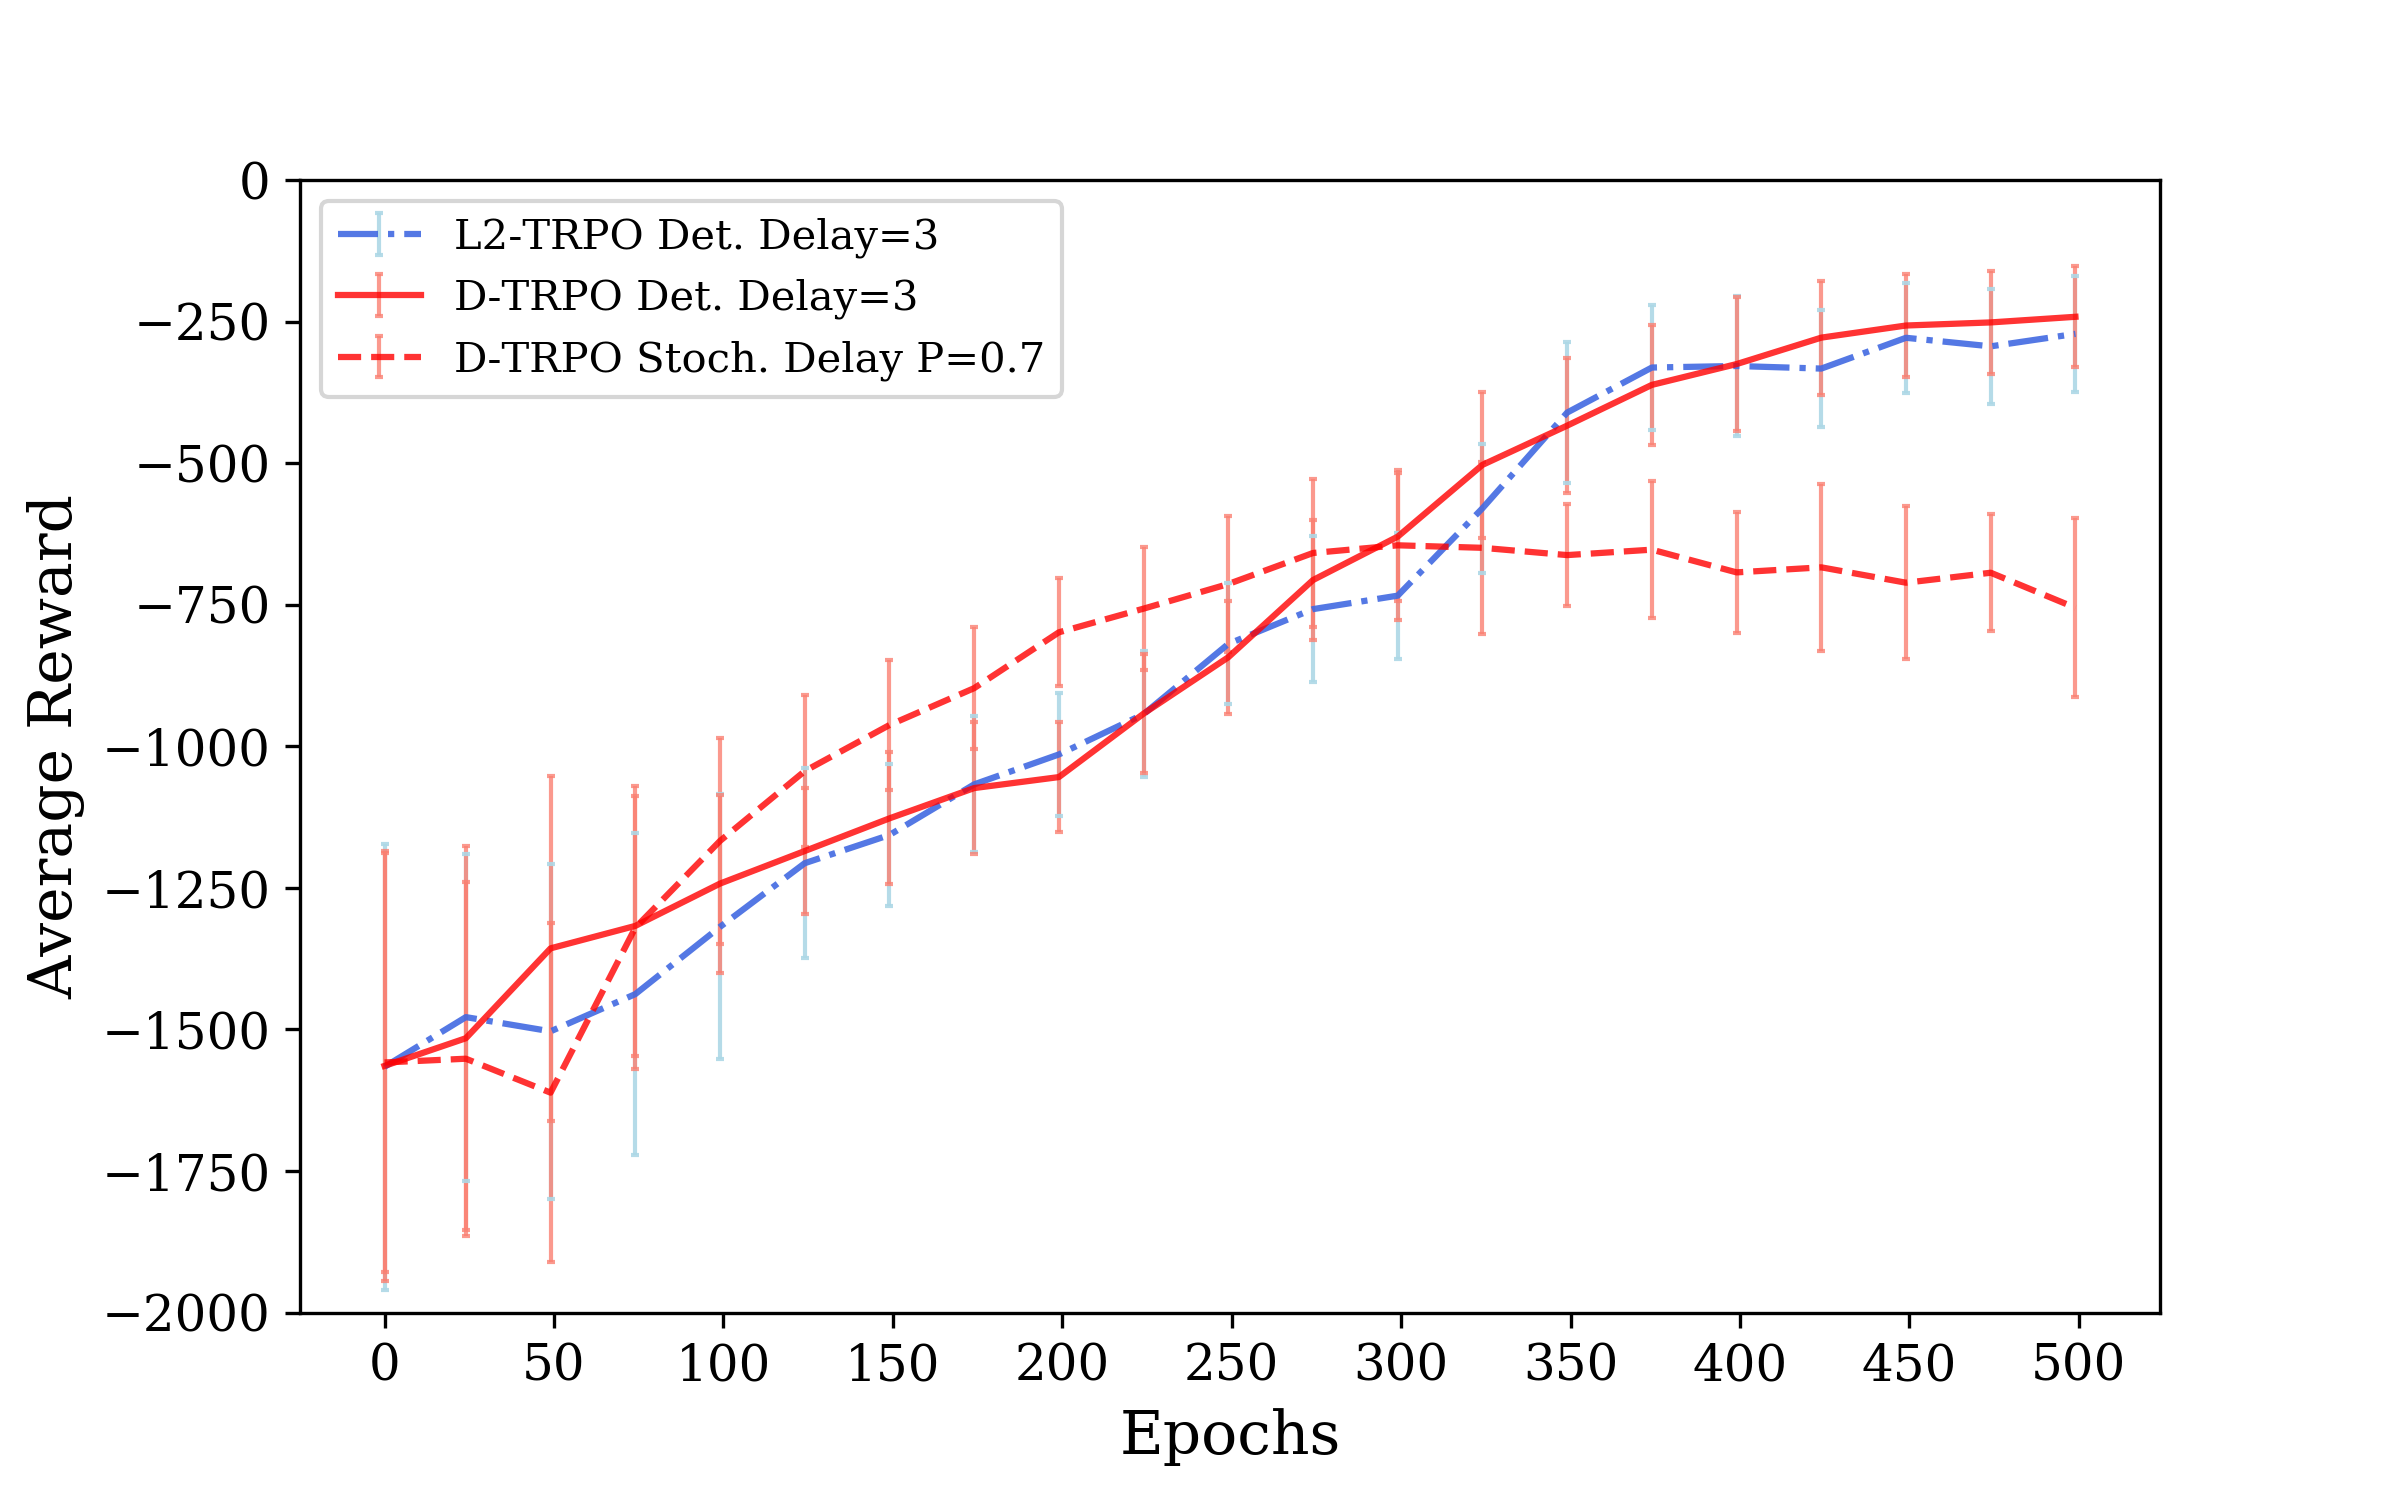
\includegraphics[width=15cm, keepaspectratio]{images/results/delayp07_comparisons_1.png}
                \caption{Training results obtained with a stochastic delay process $p=0.7$ and deterministic environment setting.}
                \label{fig:results_delayp07_1}
            \end{figure}
            
            \begin{figure}[hbtp]
                \centering
                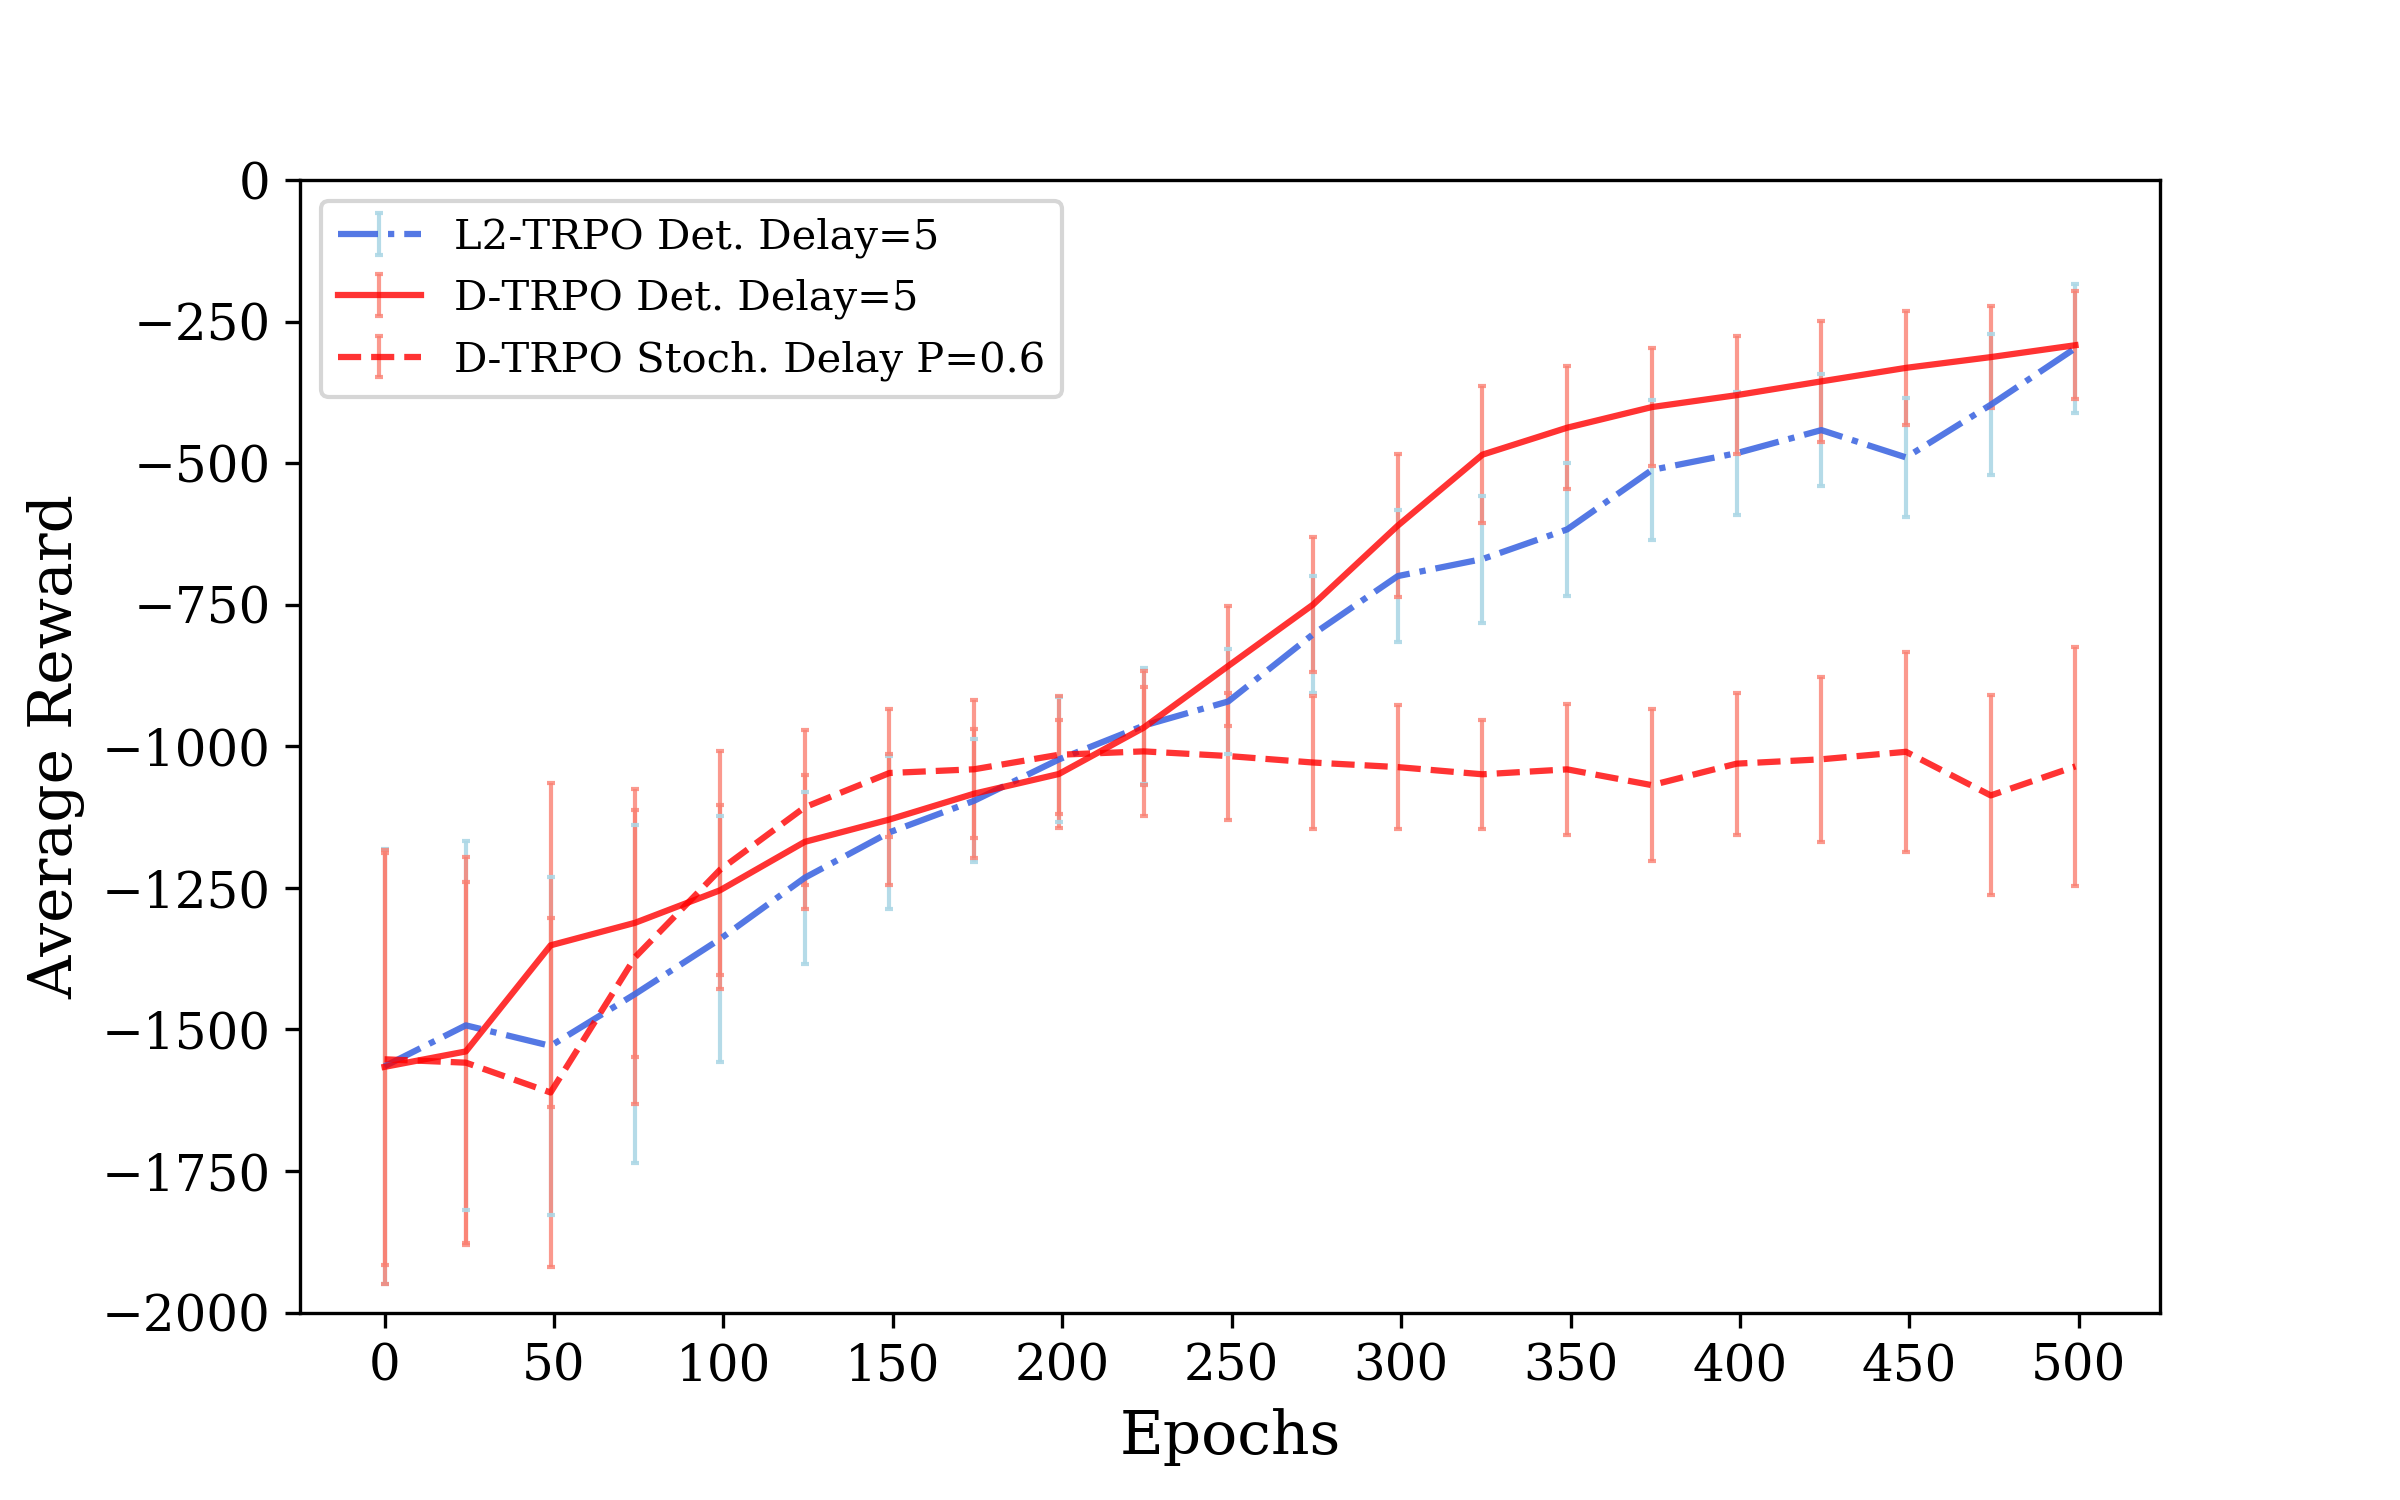
\includegraphics[width=15cm, keepaspectratio]{images/results/delayp06_comparisons_1.png}
                \caption{Training results obtained with a stochastic delay process $p=0.6$ and deterministic environment setting.}
                \label{fig:results_delayp06_1}
                
                \vspace{1.5cm}
                
                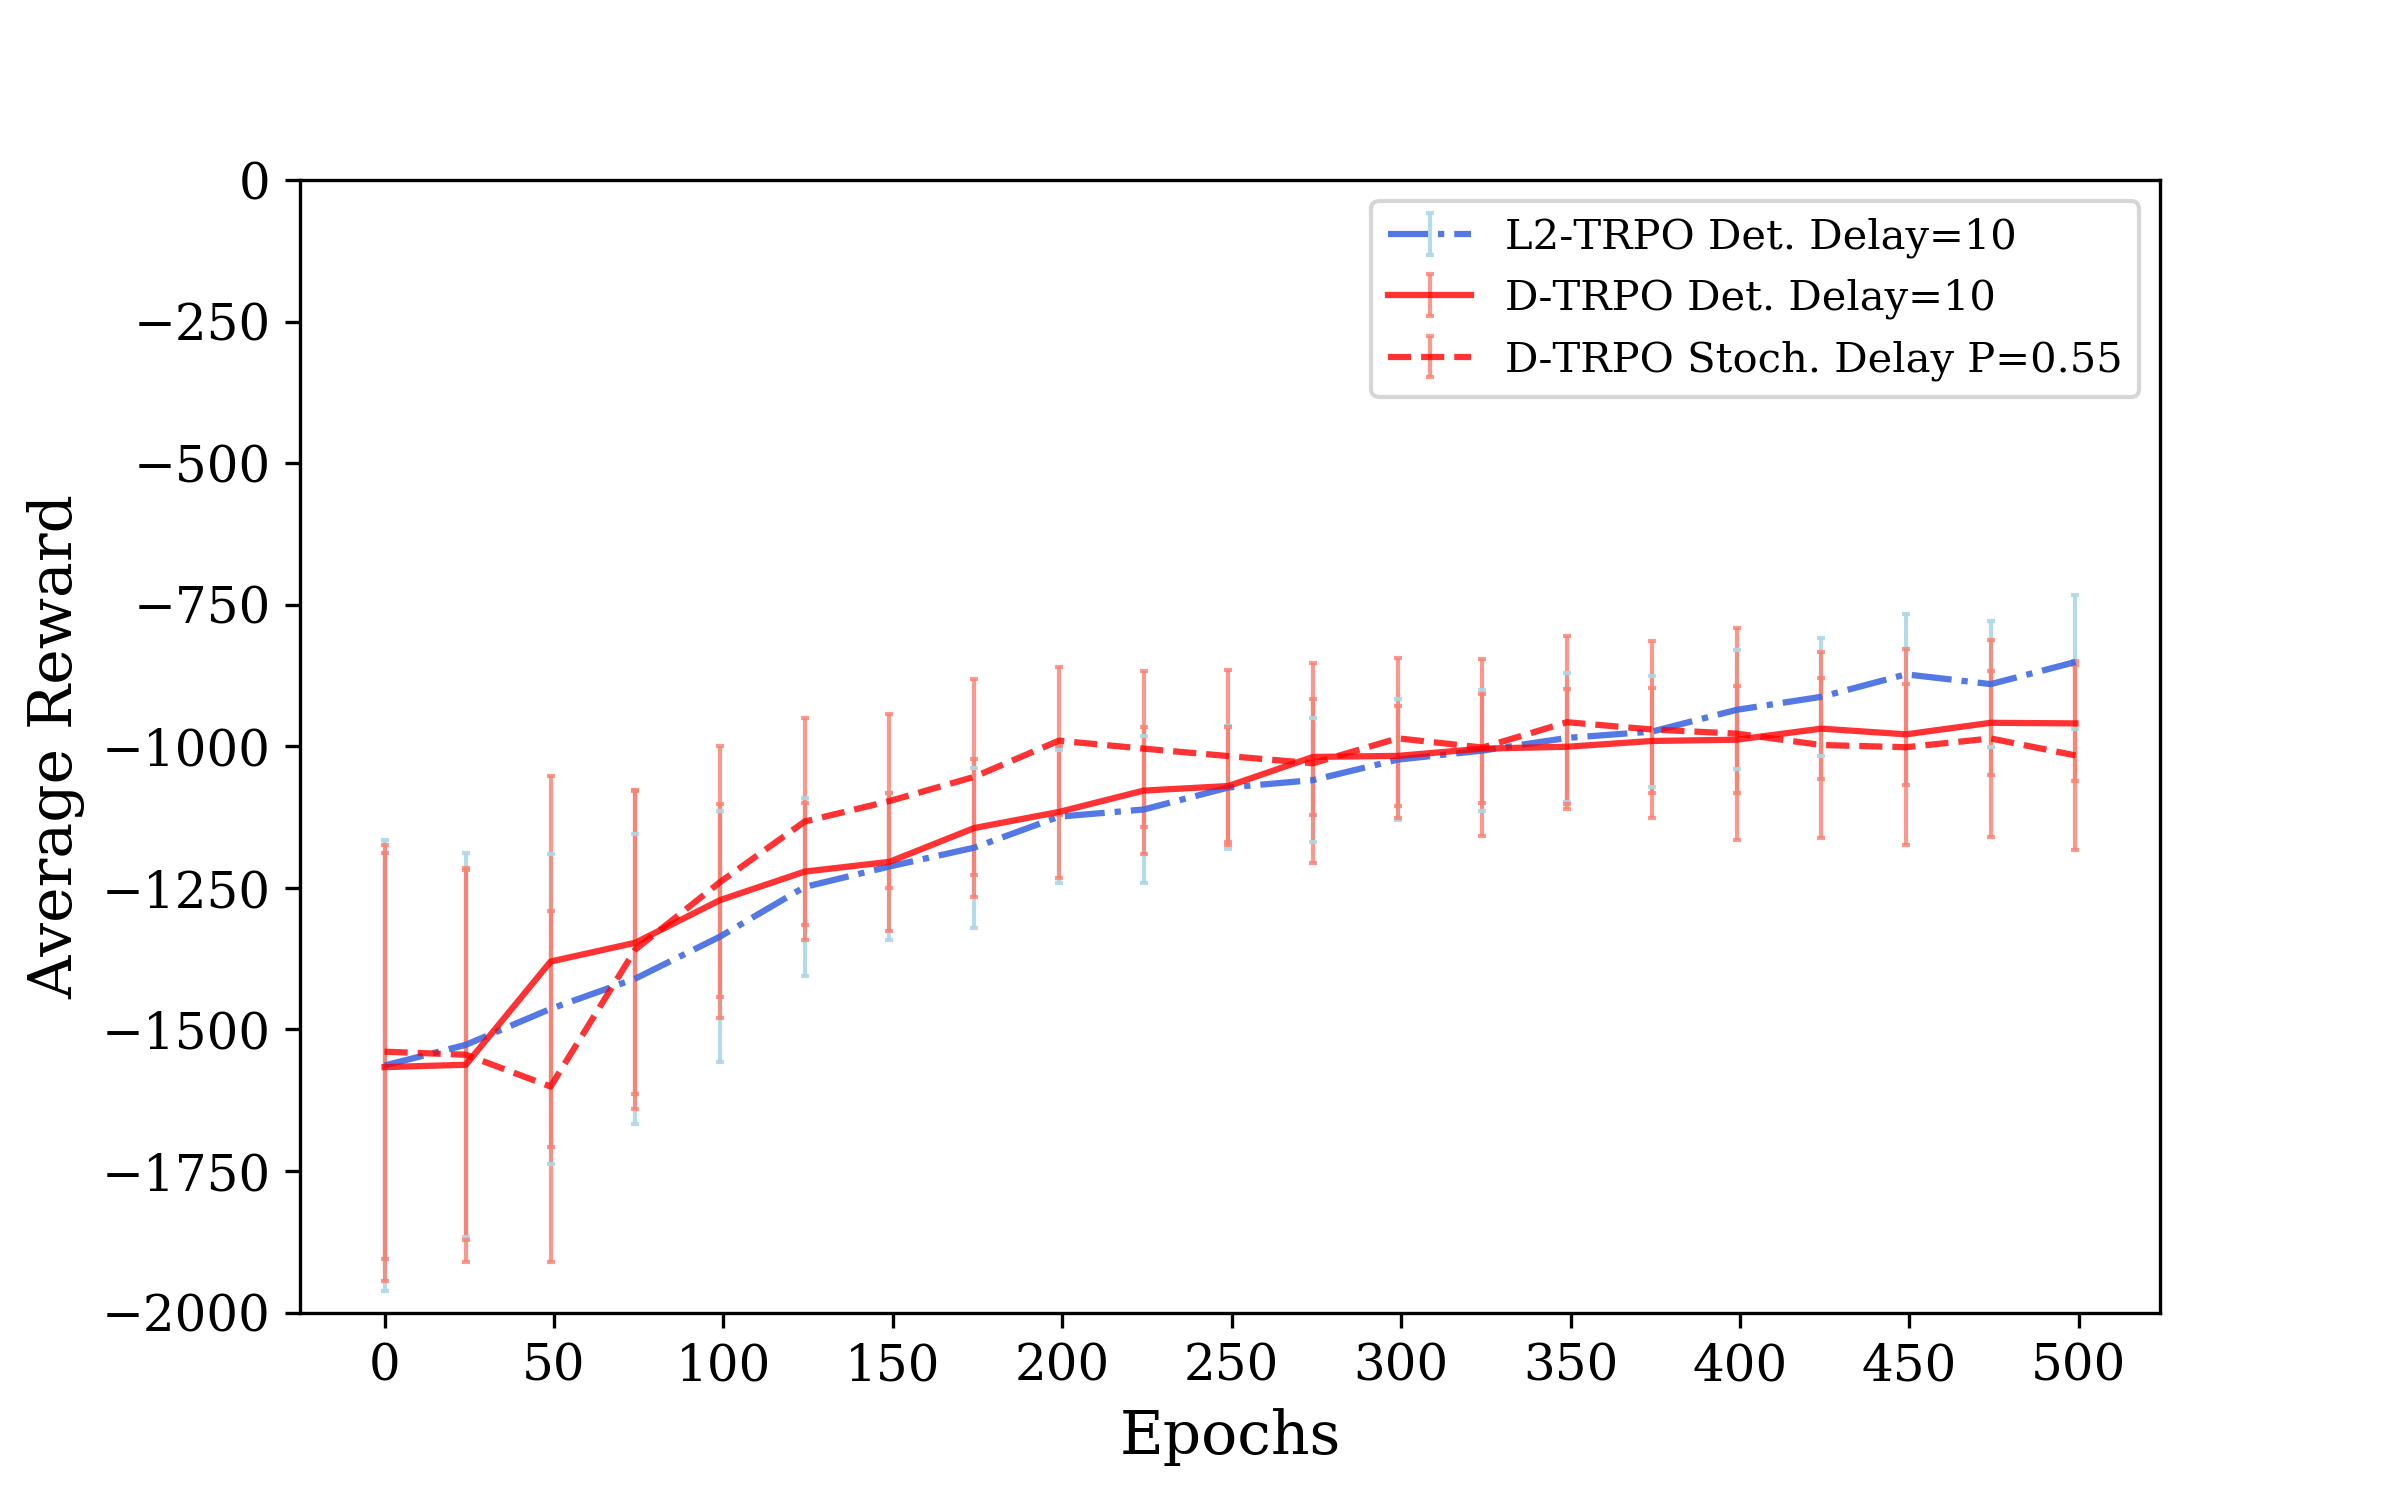
\includegraphics[width=15cm, keepaspectratio]{images/results/delayp05_comparisons_1.png}
                \caption{Training results obtained with a stochastic delay process $p=0.55$ and deterministic environment setting.}
                \label{fig:results_delayp05_1}
            \end{figure}
        
        \newpage
        \subsection{Test Results}
        \label{sub:res_test_delays}
            % Describe the behaviour of the trained models when tested on different delays w.r.t. the one they were trained with, both DTRPO and L2TRPO
            One of the strongest aspect of the proposed module is its compatibility with variable-sized input sequence, which does not only means it is possible to be trained natively with stochastic delays, but that it is also possible to test learnt model with different delay settings. In particular, we are interested in understanding how the models behave in the following two contexts:
            \begin{itemize}
                \setlength\itemsep{0.05em}
                \item The module has been trained with a certain amount of deterministic delay, but it is deployed in a setting with lower or higher deterministic delay. 
                \item The module has been trained with a certain amount of deterministic delay, but it is deployed in a stochastically delayed environment.
            \end{itemize}
            
            \subsubsection{Different Deterministic Delays Tests}
            
                \begin{table}[!b]
                    \makebox[\textwidth][c]{
                        \begin{tabular}{@{}ccccc@{}}
                        \toprule
                        \multicolumn{1}{c}{Test Setup} & 3-Steps Delay         & 5-Steps Delay        & 10-Steps Delay        & 15-Steps Delay        \\ \midrule
                        3-Steps Delay                  & -168.13 $\pm$ 102.28  & -793.21 $\pm$ 160.0  & -1210.73 $\pm$ 83.8   & -1554.17 $\pm$ 96.41  \\
                        5-Steps Delay                  & -171.12 $\pm$ 93.01   & -173.79 $\pm$ 92.2   & -1284.35 $\pm$ 85.96  & -1473.35 $\pm$ 110.78 \\
                        10-Steps Delay                 & -256.76 $\pm$ 110.75  & -246.86 $\pm$ 117.75 & -368.42 $\pm$ 126.98  & -1342.76 $\pm$ 170.88 \\
                        15-Steps Delay                 & -917.9 $\pm$ 87.04    & -902.22 $\pm$ 85.35  & -871.62 $\pm$ 102.85  & -956.13 $\pm$ 104.48  \\ \bottomrule
                        \end{tabular}
                    }
                    \centering
                    \caption{L2-TRPO trained on deterministic delays, denoted in the rows header, and Tested on deterministic delays, denoted in the columns header.}
                    \label{tab:l2trpo_det_det}
                \end{table}
                
                \begin{table}[!b]
                    \makebox[\textwidth][c]{
                        \begin{tabular}{@{}ccccc@{}}
                        \toprule
                        \multicolumn{1}{c}{Test Setup} & 3-Steps Delay         & 5-Steps Delay           & 10-Steps Delay          & 15-Steps Delay        \\ \midrule
                        3-Steps Delay                  & -155.61  $\pm$ 79.02  & -831.79 $\pm$ 127.55    & -1223.33 $\pm$ 71.02    & -1631.23 $\pm$ 77.32  \\
                        5-Steps Delay                  & -544.46  $\pm$ 105.17 & -175.36  $\pm$ 95.01    & -1161.79 $\pm$ 71.96    & -1578.53 $\pm$ 100.6  \\
                        10-Steps Delay                 & -1120.52 $\pm$ 56.54  & -1054.0  $\pm$ 65.79    & -720.49  $\pm$ 93.85    & -1352.81 $\pm$ 105.87 \\
                        15-Steps Delay                 & -1196.11 $\pm$ 66.82  & -1139.92 $\pm$ 83.66    & -1103.9  $\pm$ 76.88    & -912.31  $\pm$ 93.59  \\ \bottomrule
                        \end{tabular}
                    }
                    \centering
                    \caption{D-TRPO trained on deterministic delays, denoted in the rows header, and tested on deterministic delays, denoted in the columns header}
                    \label{tab:dtrpo_det_det}
                \end{table}
                
                Presented in Table \ref{tab:l2trpo_det_det}, L2-TRPO results are straightforward: each model trained with a certain amount of delay is also able to perform as well when tested on smaller delays, but it is not able to perform at all when tested on larger delays. This behaviour results from the definition of L2-TRPO loss function, which optimizes the module towards predictions of each unobserved state $s_{t-d+i}$, with $1 \leq i \leq d$, the Agent has traversed after the last observed state $s_{t-d}$, rather than only predicting the current unobserved state $s_t$. \newline
                D-TRPO shows a similar behaviour but its performances on smaller delays, albeit better than on larger delays, are significantly affected. Results are shown in Table \ref{tab:dtrpo_det_det}. The main reason behind this behavior lies in the interaction between the Belief-Estimation module and the policy/value networks. During training, the module takes as input extended states of the same size at each time-step and the output belief representation handled to policy/value networks reflects this property in its structure. Conceptually speaking, changing the size of the extended states has the same effect on the belief representation as changing language in a translation: for example, if D-TRPO is trained with 10 steps of delay, the learnt belief representations are built in a "10-steps-delay" language. Policy and value networks learn the belief representations in this particular "language" and they are able to improve the Agent's performances during training. However, this test is specifically targeting this assumption by letting the models interact against environments with a different delays. The results is that the module is outputting a belief representation that may be correct, but it's in a different "language" than policy and value networks expect and the Agent is not able to act accordingly. \newline
                At last, it is also possible to observe that, for both D-TRPO and L2-TRPO, in order to obtain the best possible performance we need to train the model with the same exact number of delay steps, thus confirming results from \pcite{delay:ssbm}, presented in Section \ref{subs:modelbasedapproach}.
                
            \subsubsection{Stochastic Delays Tests}
            
                \begin{table}[!b]
                    \centering
                    \begin{tabular}{@{}cccc@{}}
                    \toprule
                    \multicolumn{1}{c}{Test Setup} & Delay P=0.7           & Delay P=0.6          & Delay P=0.55         \\ \midrule
                    3-Steps Delay                  & -341.51 $\pm$ 131.67  & -609.37 $\pm$ 197.77 & -855.96 $\pm$ 238.89 \\
                    5-Steps Delay                  & -222.01 $\pm$ 118.2   & -430.42 $\pm$ 195.56 & -715.21 $\pm$ 262.44 \\
                    10-Steps Delay                 & -254.52 $\pm$ 147.07  & -306.1  $\pm$ 159.17 & -464.1  $\pm$ 235.38 \\
                    15-Steps Delay                 & -896.88 $\pm$ 78.9    & -903.66 $\pm$ 83.73  & -913.02 $\pm$ 109.81 \\ \bottomrule
                    \end{tabular}
                    \centering
                    \caption{L2-TRPO trained on deterministic delays, denoted in the rows header, and tested on stochastic delays, denoted in the columns header.}
                    \label{tab:l2trpo_det_stoch}
                \end{table}
                
                \begin{table}[!b]
                    \centering
                    \begin{tabular}{@{}cccc@{}}
                    \toprule
                    \multicolumn{1}{c}{Test Setup} & Delay P=0.7           & Delay P=0.6            & Delay P=0.55          \\ \midrule
                    3-Steps Delay                  & -344.15 $\pm$ 149.93  & -610.1 $\pm$ 196.71    & -883.26 $\pm$ 226.18  \\
                    5-Steps Delay                  & -605.38 $\pm$ 112.22  & -659.11 $\pm$ 147.38   & -800.12 $\pm$ 186.03  \\
                    10-Steps Delay                 & -1100.71 $\pm$ 68.2   & -1055.5 $\pm$ 83.53    & -1045.56 $\pm$ 104.81 \\
                    15-Steps Delay                 & -1196.4 $\pm$ 72.23   & -1158.42 $\pm$ 81.97   & -1131.19 $\pm$ 96.66  \\ \bottomrule
                    \end{tabular}
                    \centering
                    \caption{D-TRPO trained on deterministic delays, denoted in the rows header, and tested on stochastic delays, denoted in the columns header.}
                    \label{tab:dtrpo_det_stoch}
                \end{table}
                
                L2-TRPO confirms results obtained in the previous test in Table \ref{tab:l2trpo_det_stoch}. When a L2-TRPO model is tested with a stochastic delay process whose samples are generally less than or equal to the training constant delay, the module is able to build precise state predictions and the model is able to perform well, in some cases even close to the performances obtained when tested on deterministic delays. Lower performances across the tests are expected: the stochastic delay process is able to sample delays that are higher than the constant delay the model is trained with, thus the module is not able to provide a precise prediction at each time-step. \newline
                As expected, Table \ref{tab:dtrpo_det_stoch} shows that D-TRPO is suffering from the same issues discovered in the previous test. Performances are higher when the stochastic delay processes samples delays that are closer to the one the model has been trained with. While the 3-steps delay model is performing as well as the L2-TRPO counterpart, performances quickly decrease with both larger training delays and more difficult stochastic delay processes.
            
    \newpage
    \section{Stochastic Environment}
    \label{results:stochastic}
        % DTRPO vs L2TRPO
        This last Section is dedicated to experiments in a stochastic environment. It is divided in to two sub-section: while Section \ref{sub:stoch_noise_impl} is concerned with explaining the stochastic environment implementation, Section \ref{sub:stoch_env_res} discusses the obtained results. We tested D-TRPO and L2-TRPO, both with the same hyperparameters explained in Section \ref{results:deterministic} in an environment affected by 5 steps of delay. Models are trained for 1000 epochs, each of them composed by 5000 steps for a total of 5 million steps. Single trajectories last for 250 steps. 
        
        \subsection{Stochastic Noise Implementation}
        \label{sub:stoch_noise_impl}
        % Explain each noise
            Stochastic environment implementation is reached by adding a stochastic perturbation to the sequence of actions chosen by the Agent while interacting in the Inverted Pendulum environment. In practice, at each time-step $t$, the Agent selects an action $a_t$, a perturbation $\epsilon_t$ is sampled from a probability distribution and the action executed in the environment is $a_t + \epsilon_t$. We implemented perturbations sampled from the following probability distributions: Beta distribution with $\alpha=2$ and $\beta=2$, referred to as Quadratic; Beta distribution with $\alpha=0.5$ and $\beta=0.5$, referred to as U-Shaped; Beta distribution with $\alpha=8$ and $\beta=2$; LogNormal distribution with zero mean and both 0.1 and 1 standard deviation and a Triangular distribution in [-2, 2] with mode at 1. The shape of each distributions is shown in Figure \ref{fig:noises_all}.
        
            \begin{figure}
                \vspace{4.0cm}
                \centering
                \begin{subfigure}[b]{0.45\textwidth}
                    \centering
                    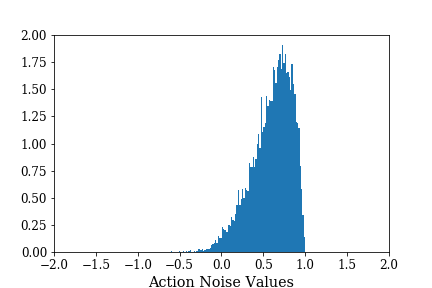
\includegraphics[width=\textwidth]{images/results/noises_beta_dist.png}
                    \caption{Shape of a Beta distribution with $\alpha=8$ and $\beta=2$.}
                    \label{fig:noises_beta_dist}
                \end{subfigure}
                \hfill
                \begin{subfigure}[b]{0.45\textwidth}
                    \centering
                    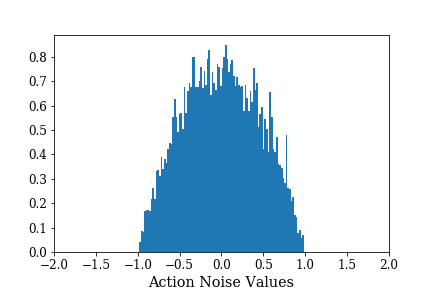
\includegraphics[width=\textwidth]{images/results/noises_quad_dist.png}
                    \caption{Shape of a Quadratic distribution (Beta with $\alpha=2$ and $\beta=2$).}
                    \label{fig:noises_quad_dist}
                \end{subfigure}
                \hfill
                \begin{subfigure}[b]{0.45\textwidth}
                    \centering
                    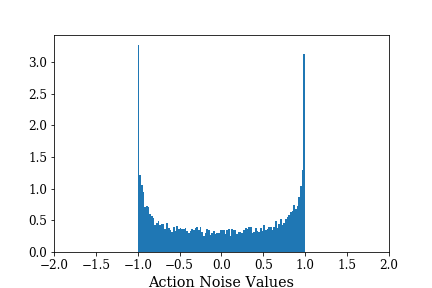
\includegraphics[width=\textwidth]{images/results/noises_ush_dist.png}
                    \caption{Shape of an U-Shaped distribution (Beta with $\alpha=0.5$ and $\beta=0.5$).}
                    \label{fig:noises_ush_dist}
                \end{subfigure}
                \hfill
                \begin{subfigure}[b]{0.45\textwidth}
                    \centering
                    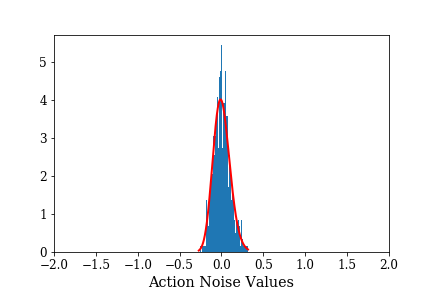
\includegraphics[width=\textwidth]{images/results/noises_logns_dist.png}
                    \caption{Shape of a LogNormal distribution with STD=0.1.}
                    \label{fig:noises_logns_dist}
                \end{subfigure}
                \hfill
                \begin{subfigure}[b]{0.45\textwidth}
                    \centering
                    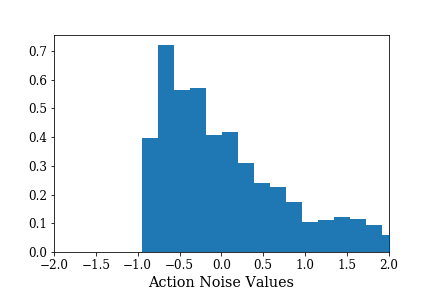
\includegraphics[width=\textwidth]{images/results/noises_logn_dist.png}
                    \caption{Shape of a LogNormal distribution with STD=1.0.}
                    \label{fig:noises_logn_dist}
                \end{subfigure}
                \hfill
                \begin{subfigure}[b]{0.45\textwidth}
                    \centering
                    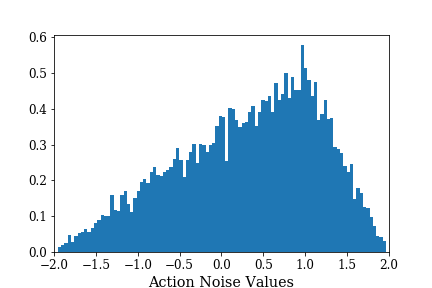
\includegraphics[width=\textwidth]{images/results/noises_tri_dist.png}
                    \caption{Shape of a Triangular distribution, with mode at 1.}
                    \label{fig:noises_tri_dist}
                \end{subfigure}
                \caption{Shape of each Perturbation distribution. }
                \label{fig:noises_all}
            \end{figure}
            
        \subsection{Results}
        \label{sub:stoch_env_res}
        % Comment results
            From Figure \ref{fig:results_beta_1} to Figure \ref{fig:results_tri_1} training results are shown along with a comparison against D-TRPO and L2-TRPO trained with the same delay in the deterministic environment, in order to observe the impact of each stochastic perturbation. Across all the stochastic perturbations, it is possible to observe a great impact in the overall performance of both D-TRPO and L2-TRPO when compared to their deterministic environment counterpart. However, it is possible to identify two different behaviour across all tests:
            \begin{itemize}
                \setlength\itemsep{0.05em}
                \item Both D-TRPO and L2-TRPO heavily suffers from the presence of the stochastic perturbation, as in the case of LogNormal with STD=1.0, U-Shaped and Triangular perturbations, and their performances are aligned;
                \item Even if the decrease of performances is evident for both algorithms, D-TRPO shows a systematic improvement w.r.t. L2-TRPO, such in the cases of Beta(8,2), Quadratic and LogNormal with STD=0.1 perturbations.
            \end{itemize}
            The latter behaviour is promising, since it reveals that D-TRPO is able to significantly outperform L2-TRPO when the stochastic perturbation is not too strong, which in turn means that the MAF network approach reveals to be beneficial w.r.t. the more standard approach of state prediction in the case of stochastic environments. 
            
            \begin{figure}[hbtp]
                \centering
                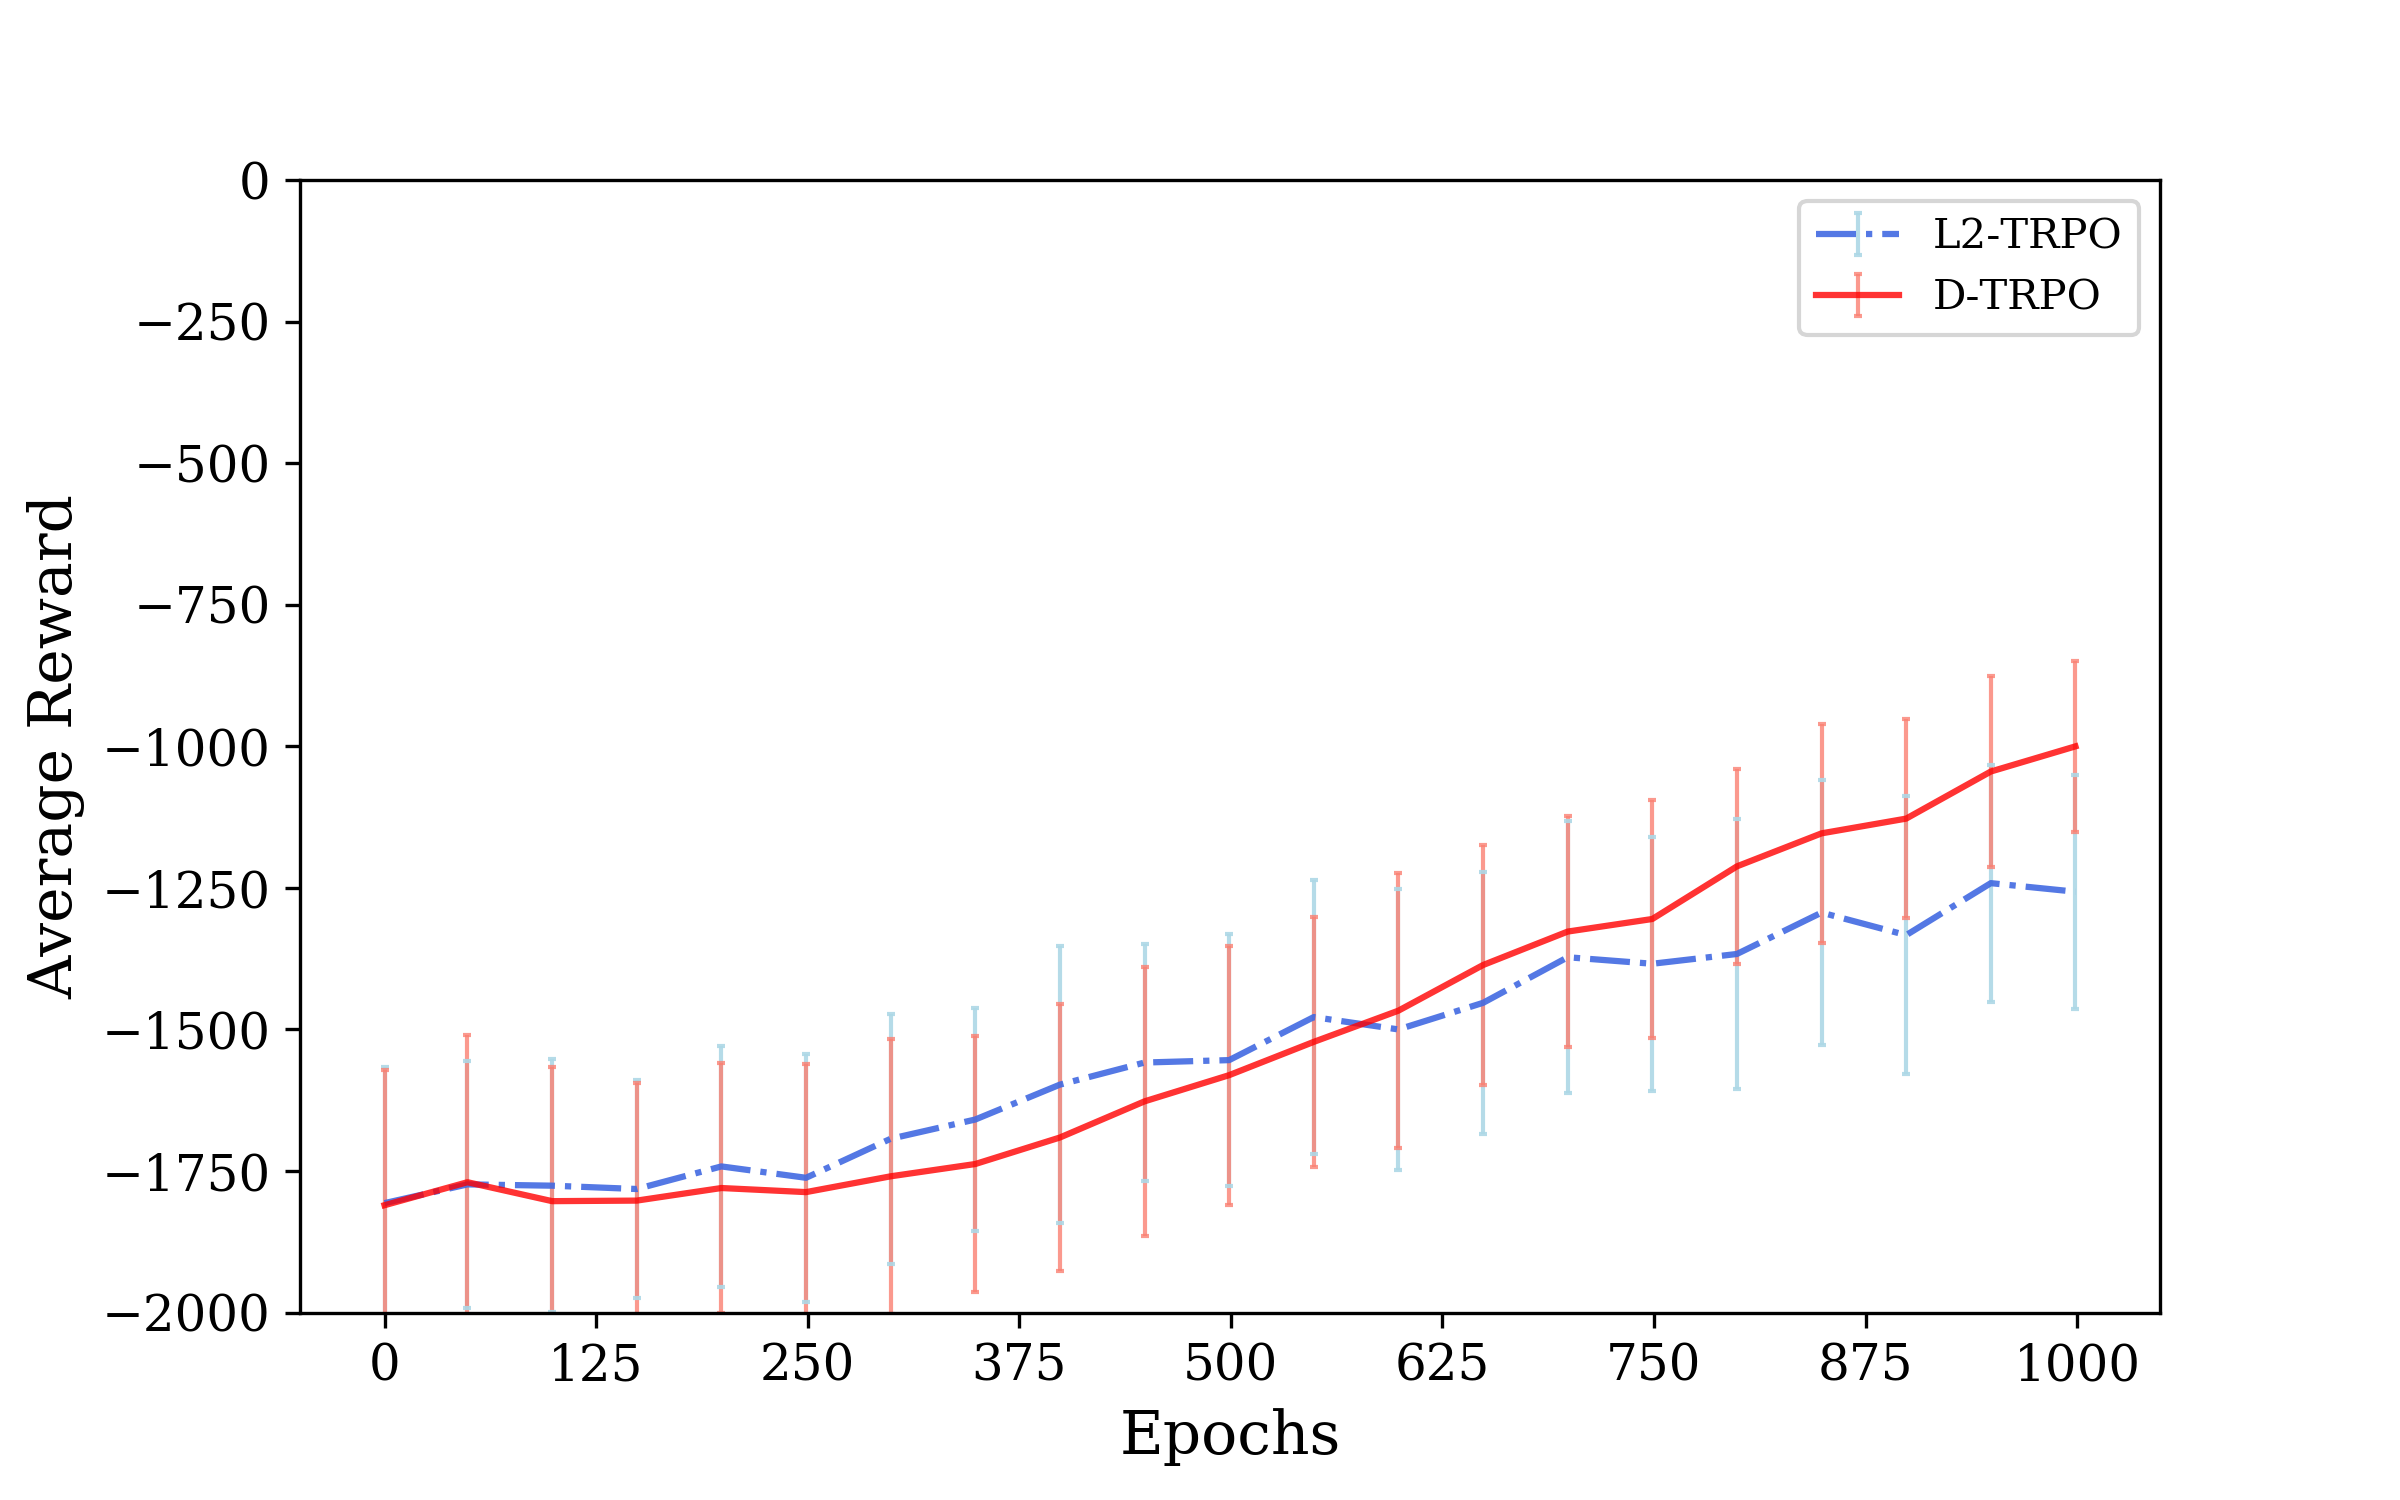
\includegraphics[width=11cm, keepaspectratio]{images/results/noises_beta_comparison_1.png}
                \caption{Training results obtained with deterministic delay of 5 steps and a Beta(8,2) perturbation.}
                \label{fig:results_beta_1}
                
                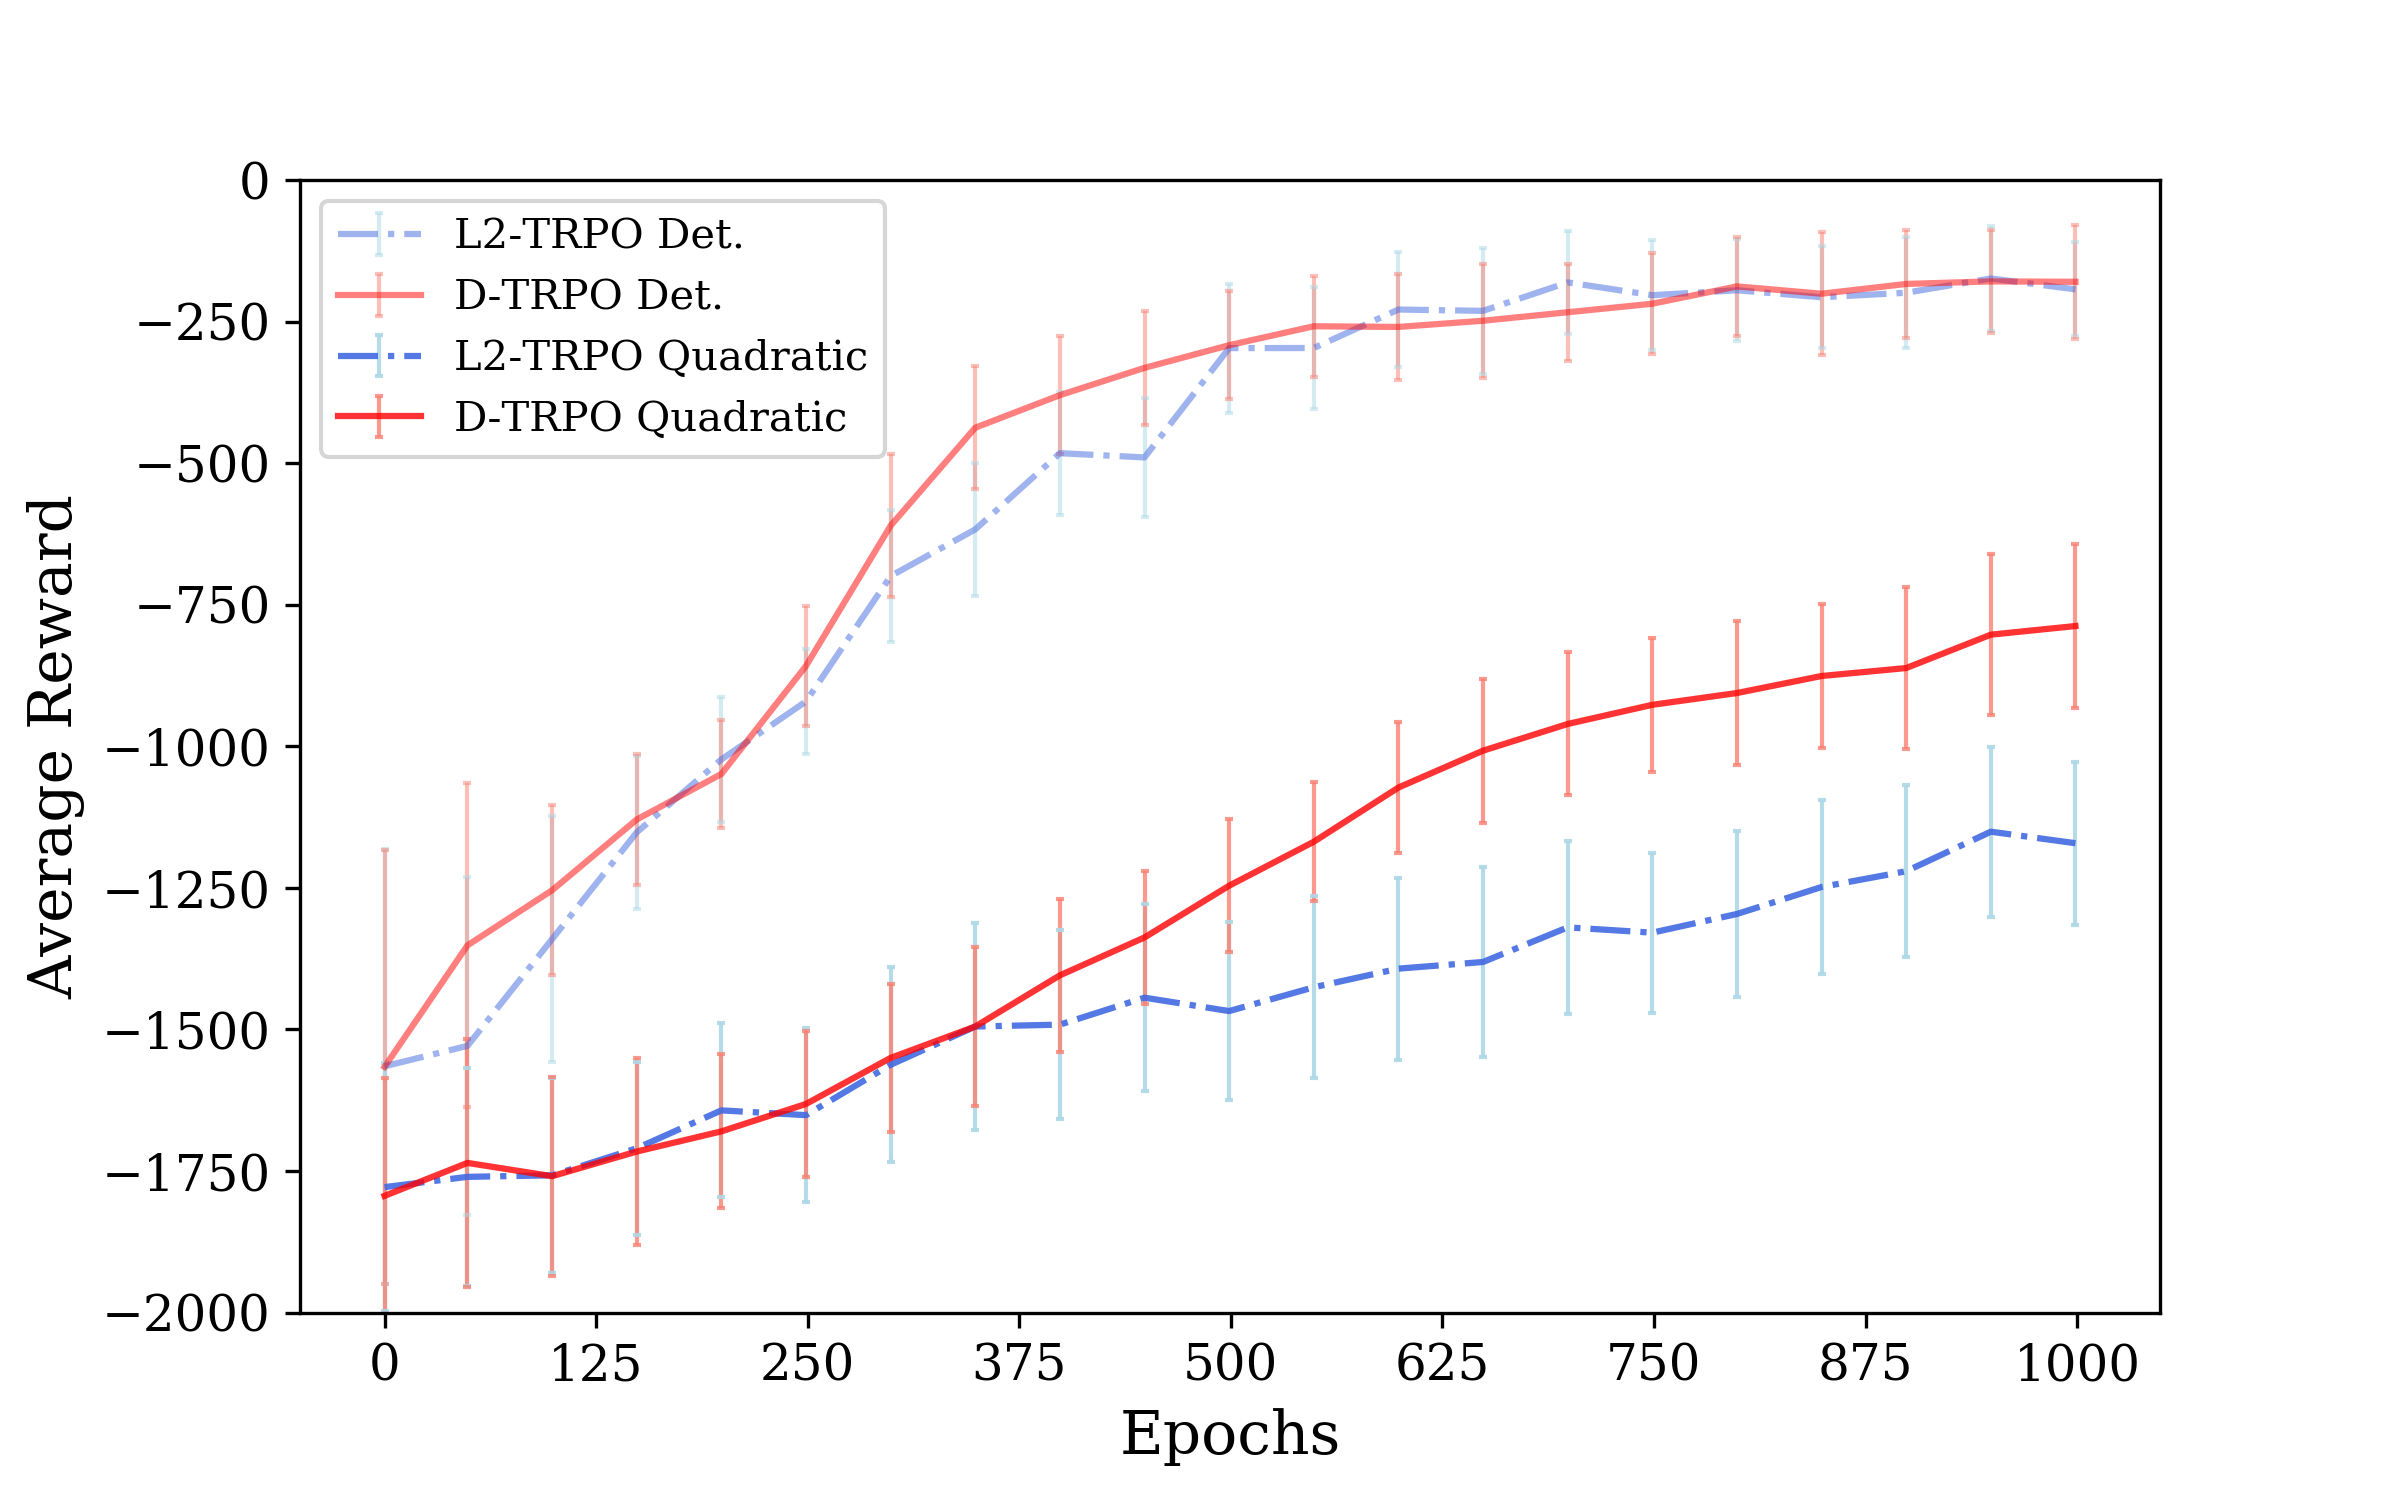
\includegraphics[width=11cm, keepaspectratio]{images/results/noises_quad_comparison_1.png}
                \caption{Training results obtained with deterministic delay of 5 steps and a Quadratic perturbation.}
                \label{fig:results_quad_1}
                
                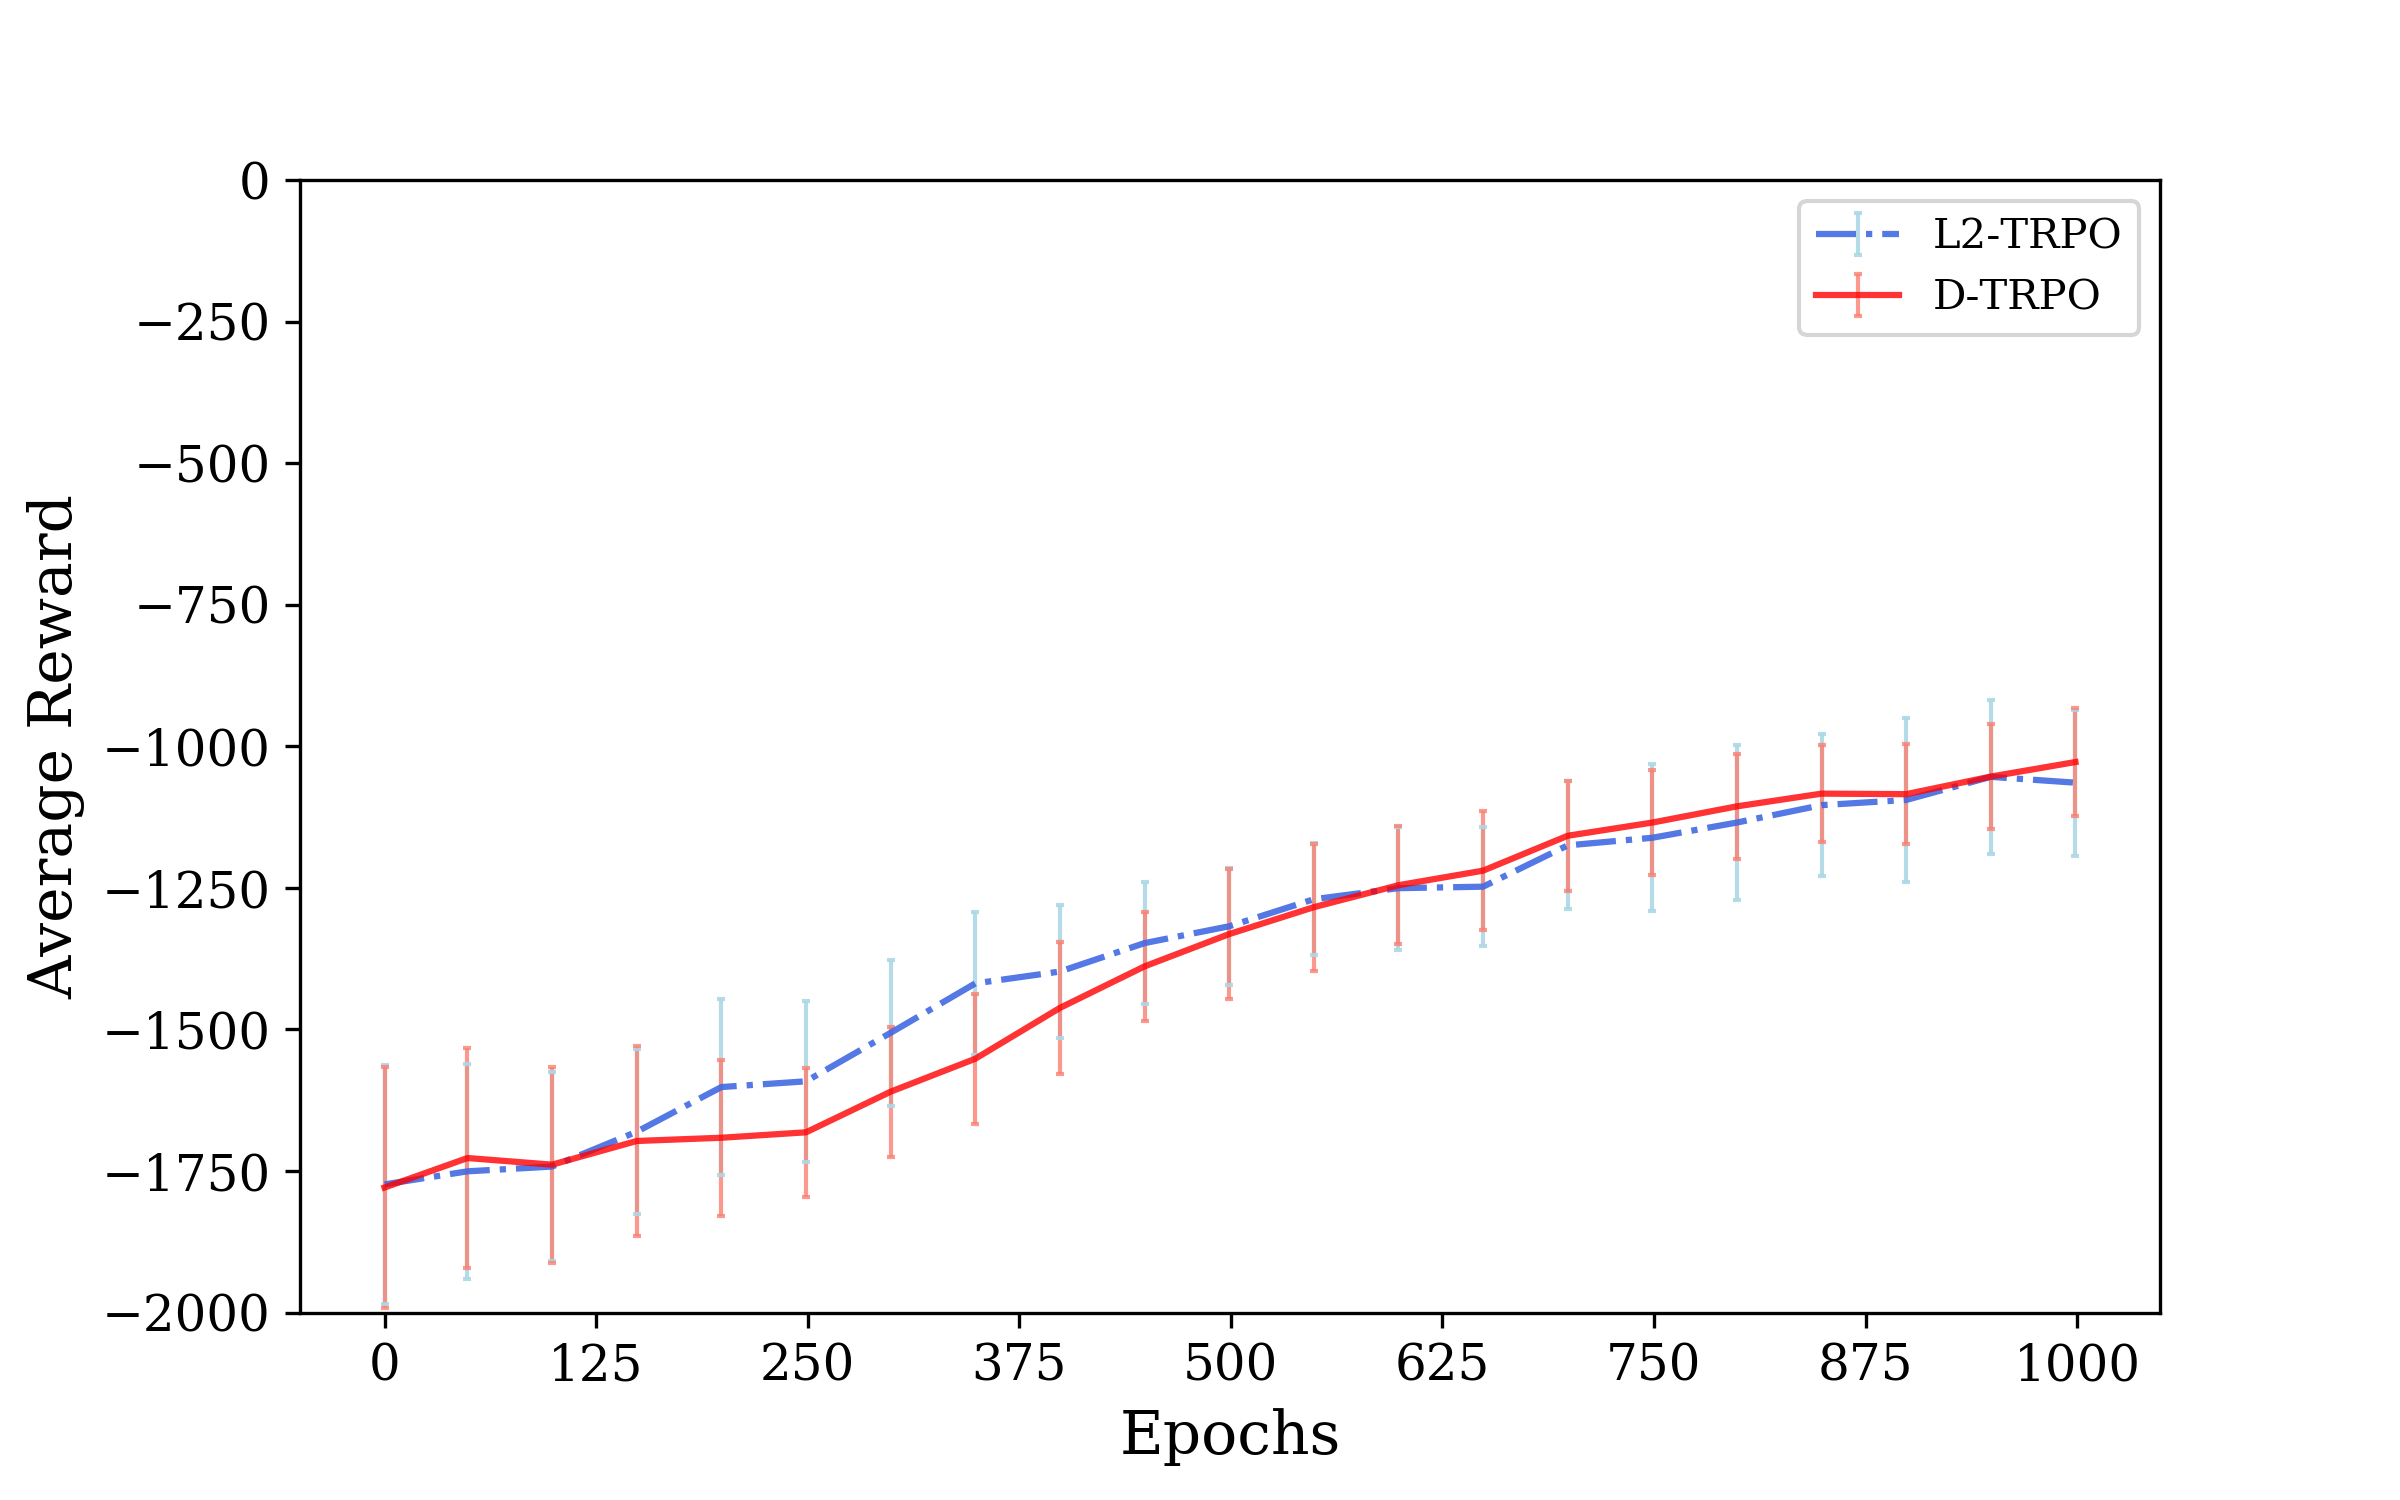
\includegraphics[width=11cm, keepaspectratio]{images/results/noises_ush_comparison_1.png}
                \caption{Training results obtained with deterministic delay of 5 steps and a U-Shaped perturbation.}
                \label{fig:results_ush_1}
            \end{figure}
            
            \begin{figure}[hbtp]
                \centering
                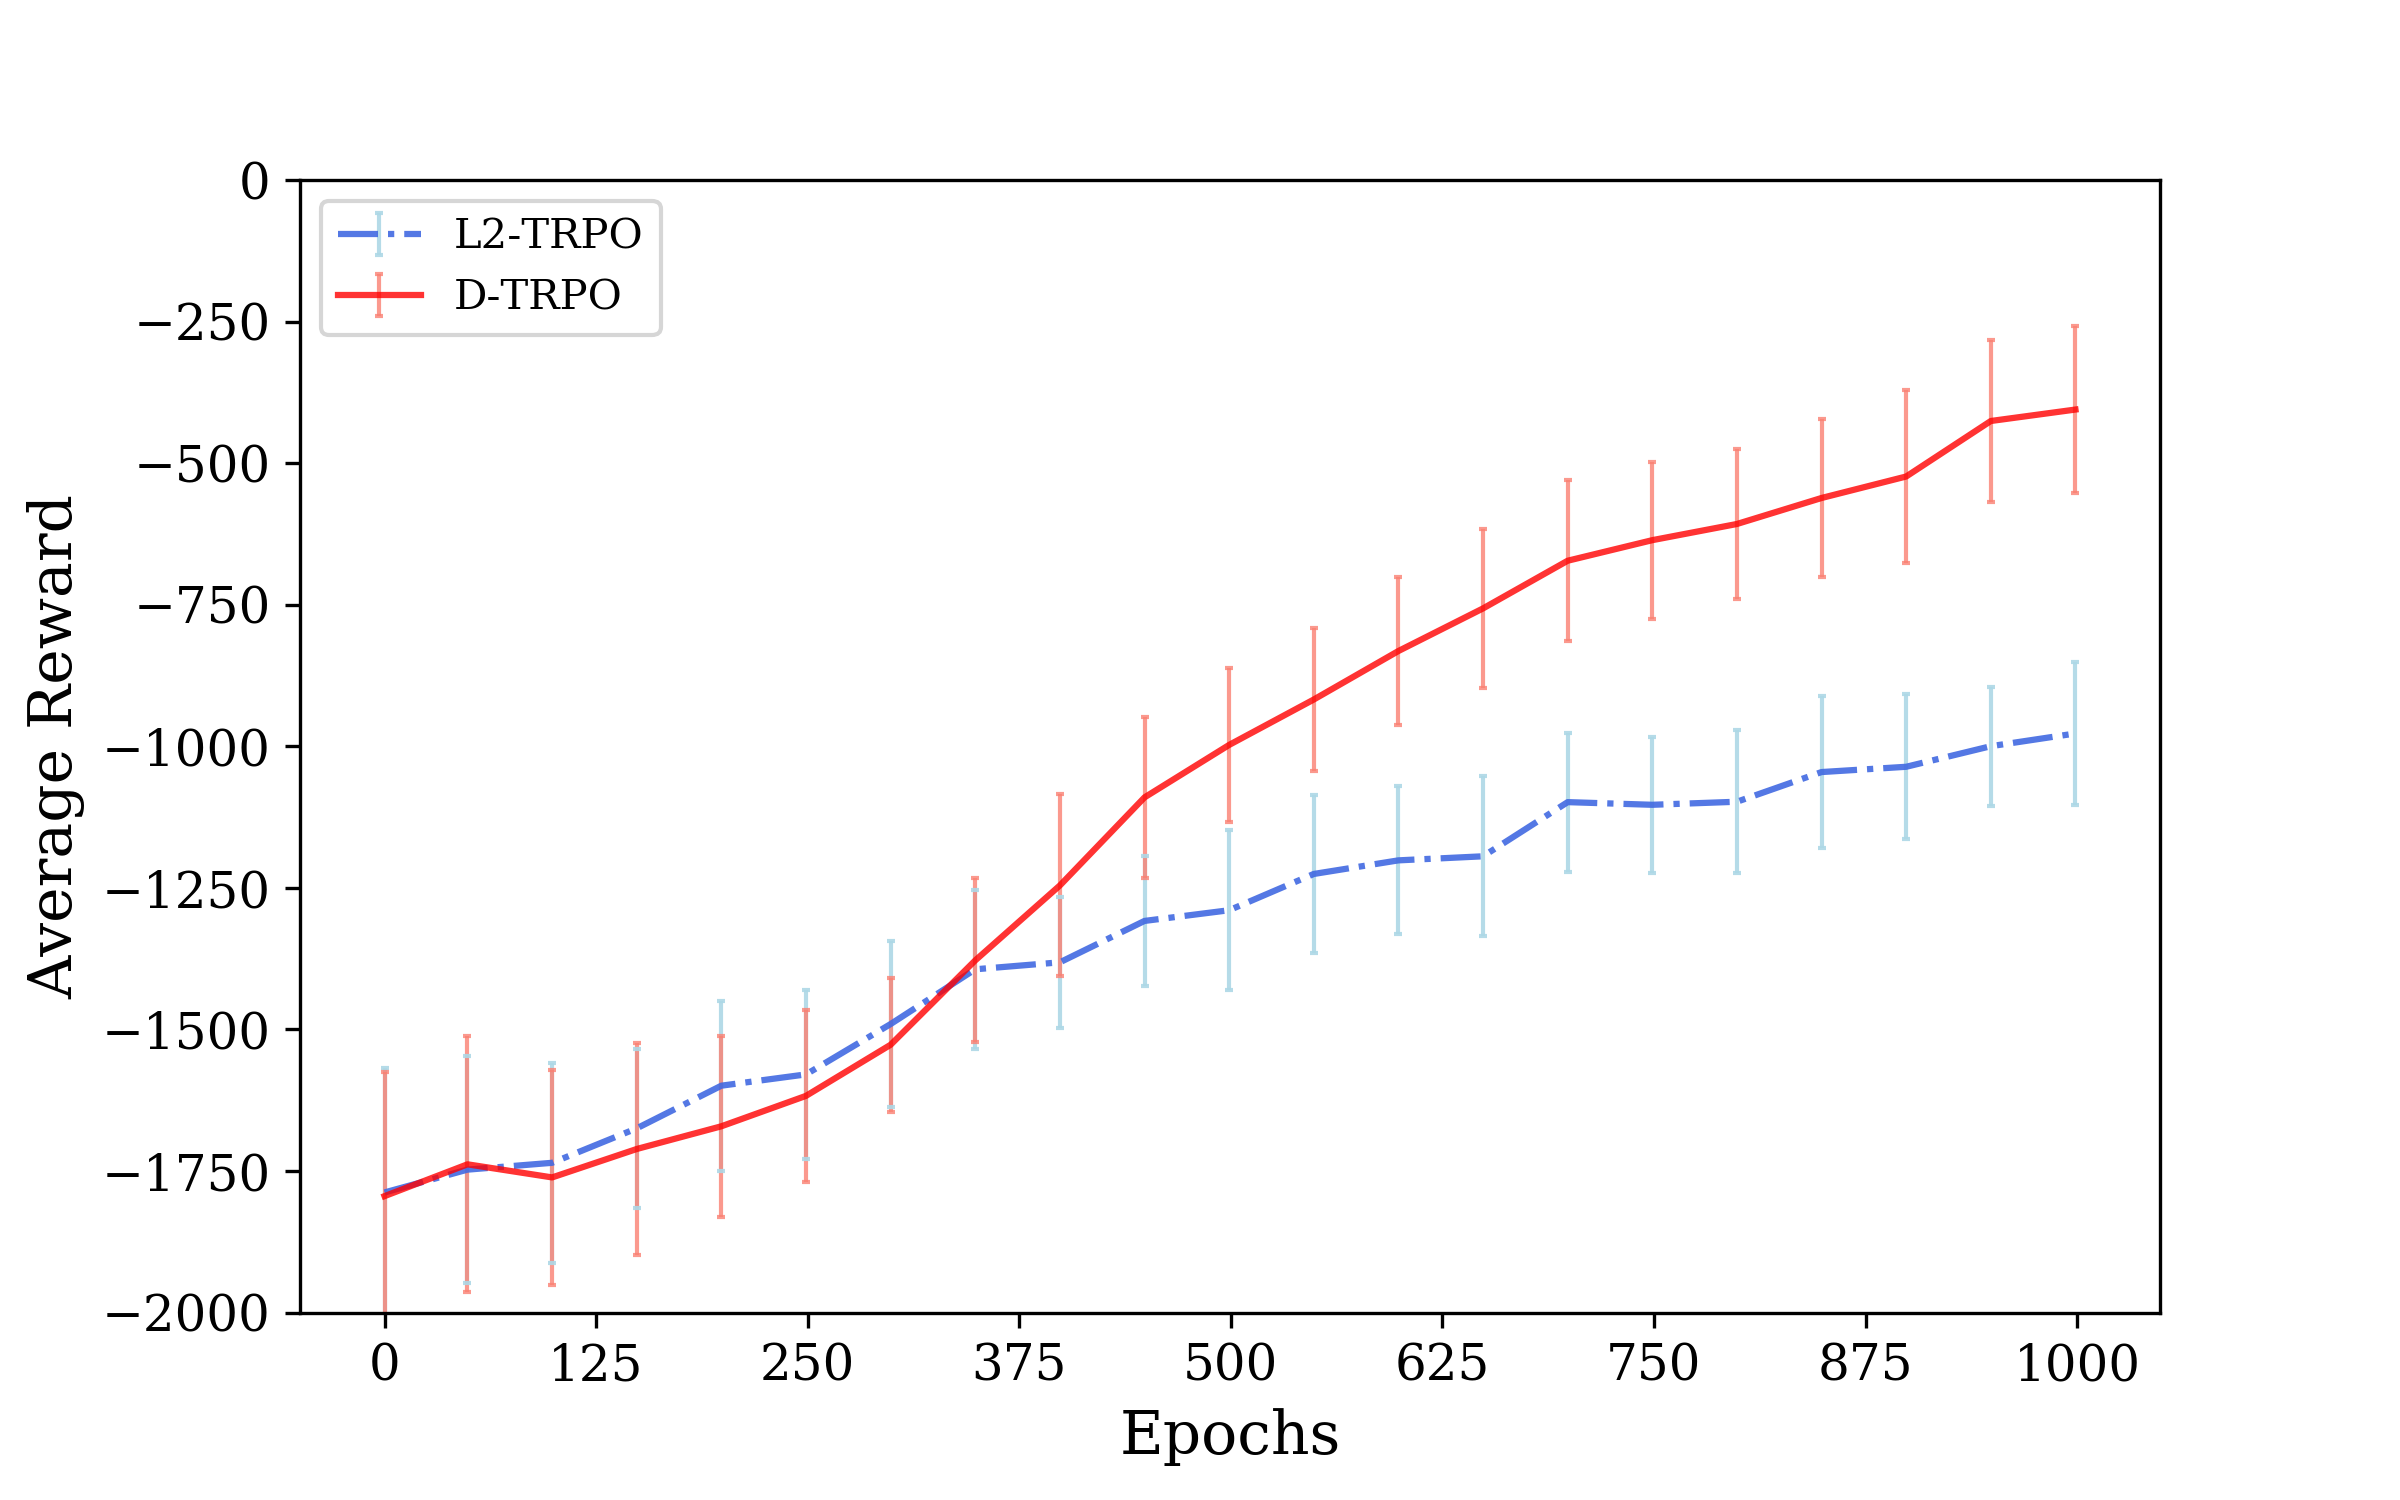
\includegraphics[width=11cm, keepaspectratio]{images/results/noises_logns_comparison_1.png}
                \caption{Training results obtained with deterministic delay of 5 steps and a LogNormal perturbation with STD=0.1.}
                \label{fig:results_logns_1}
                
                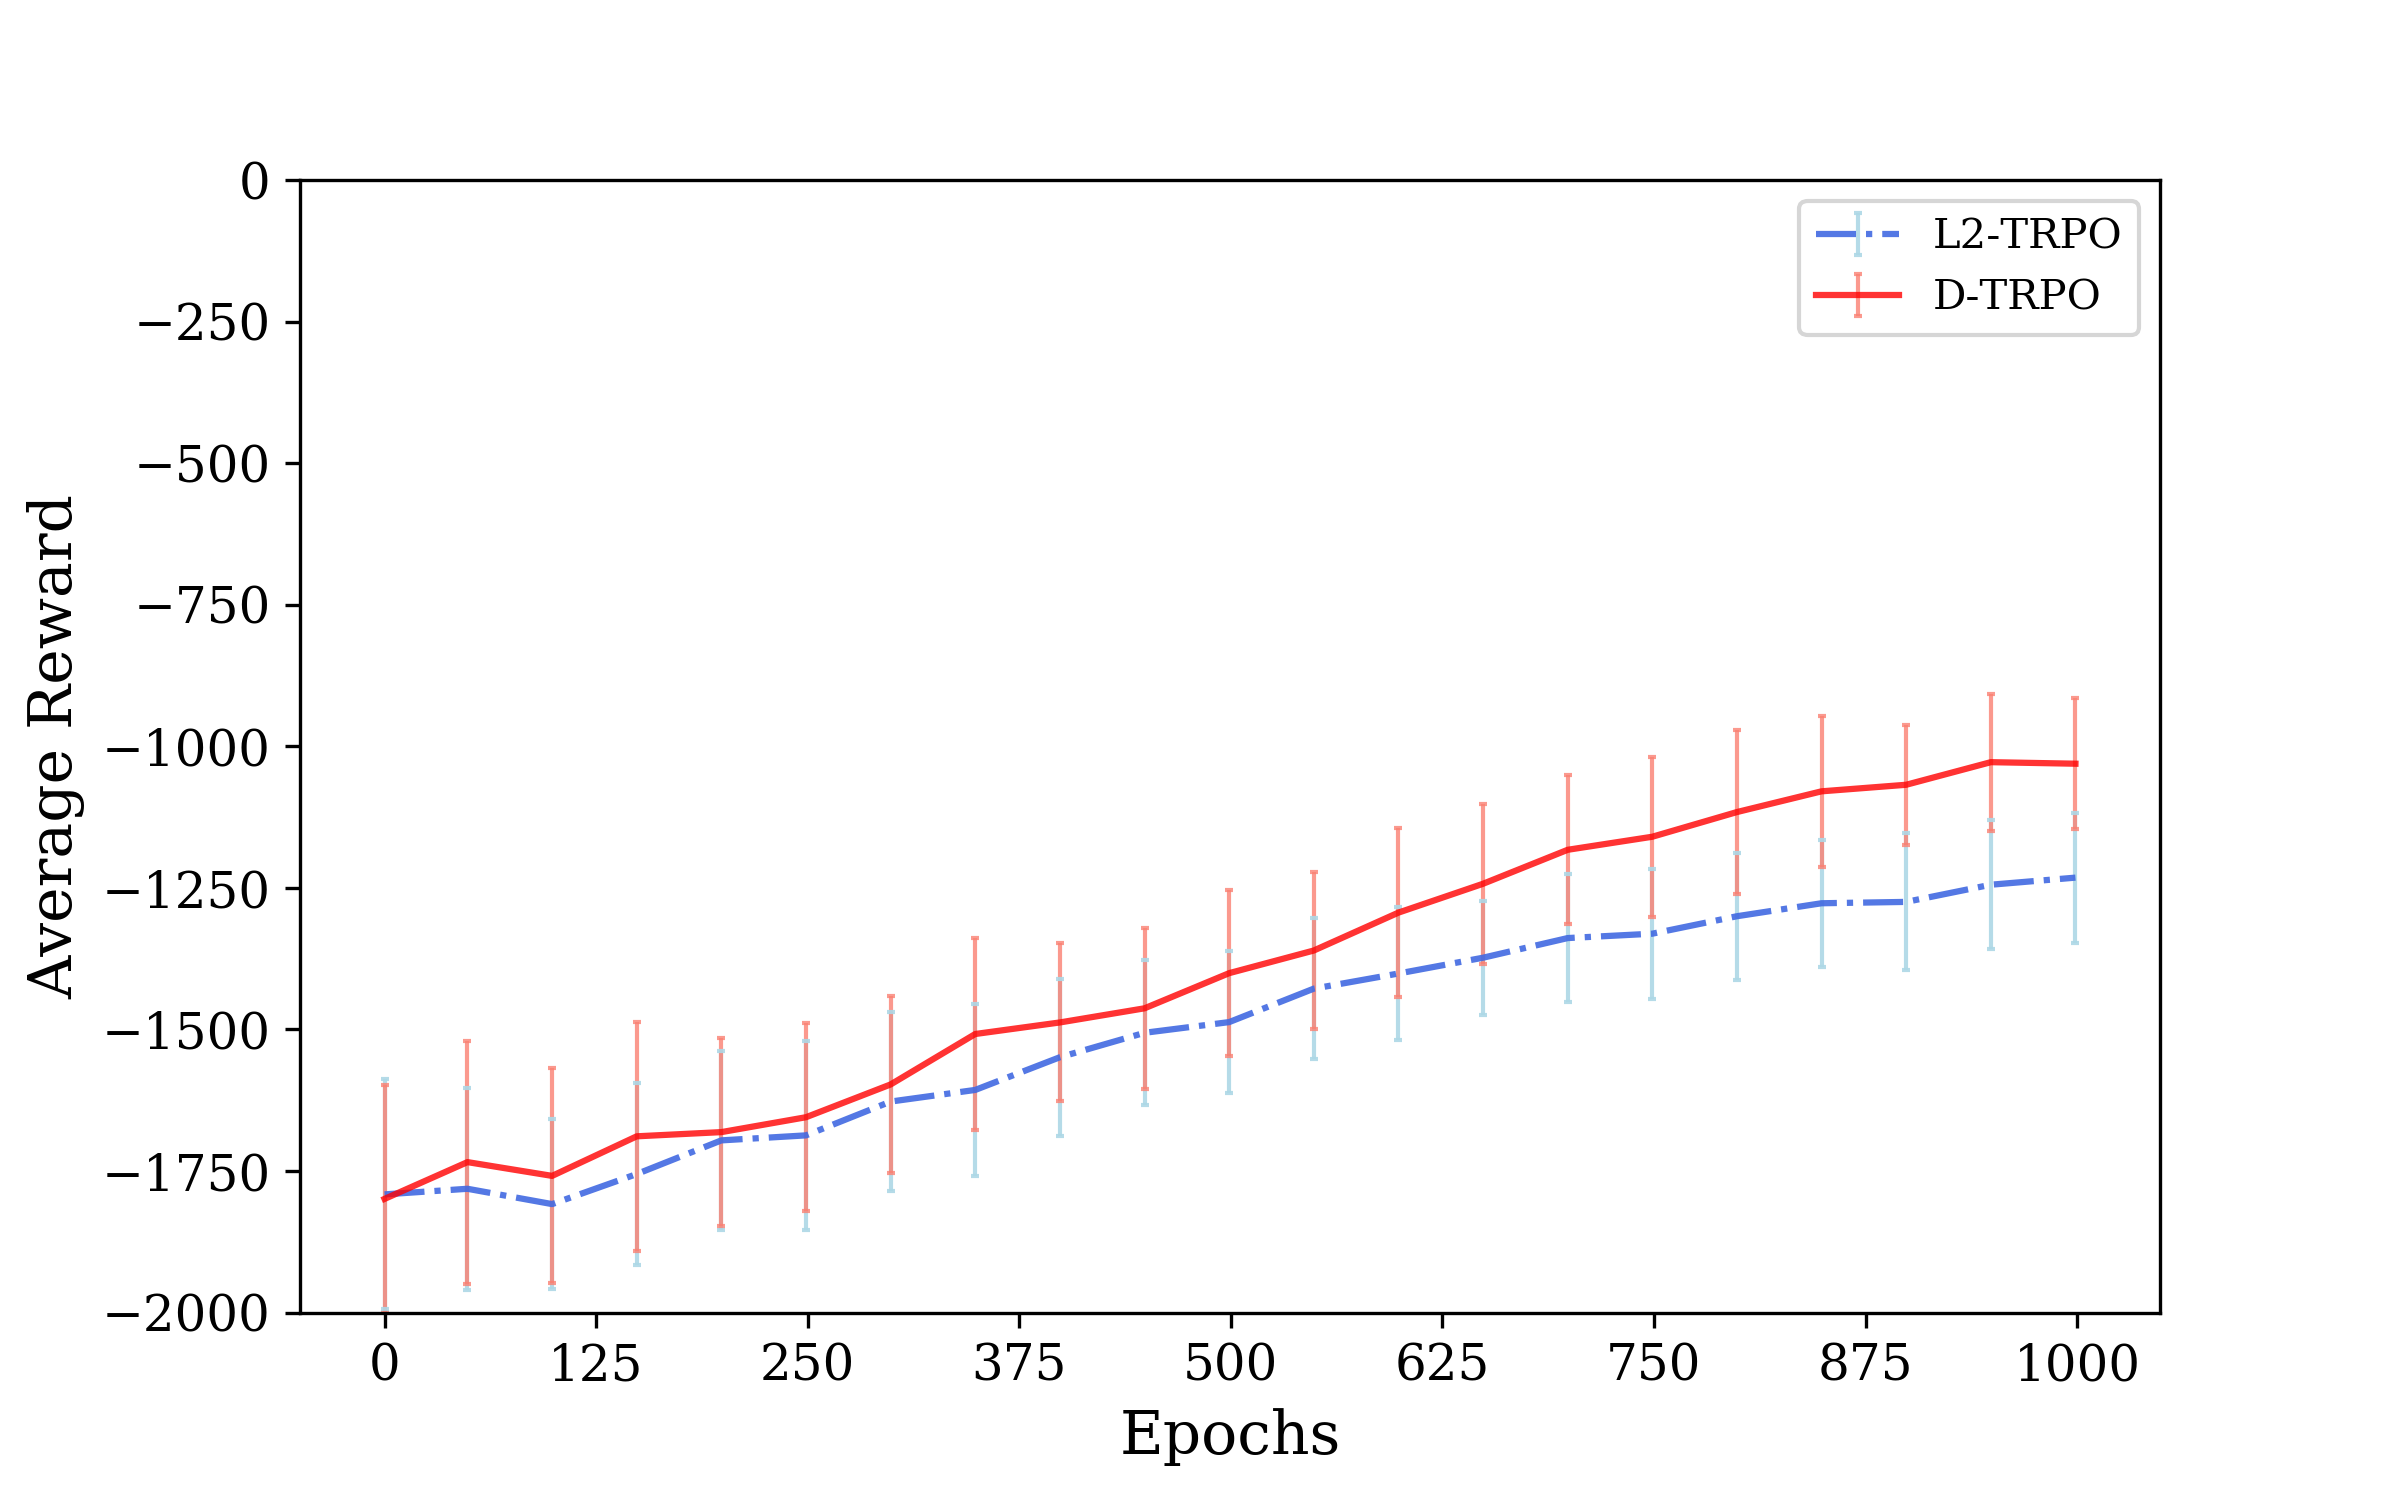
\includegraphics[width=11cm, keepaspectratio]{images/results/noises_logn_comparison_1.png}
                \caption{Training results obtained with deterministic delay of 5 steps and a LogNormal perturbation with STD=1.0.}
                \label{fig:results_logn_1}
                
                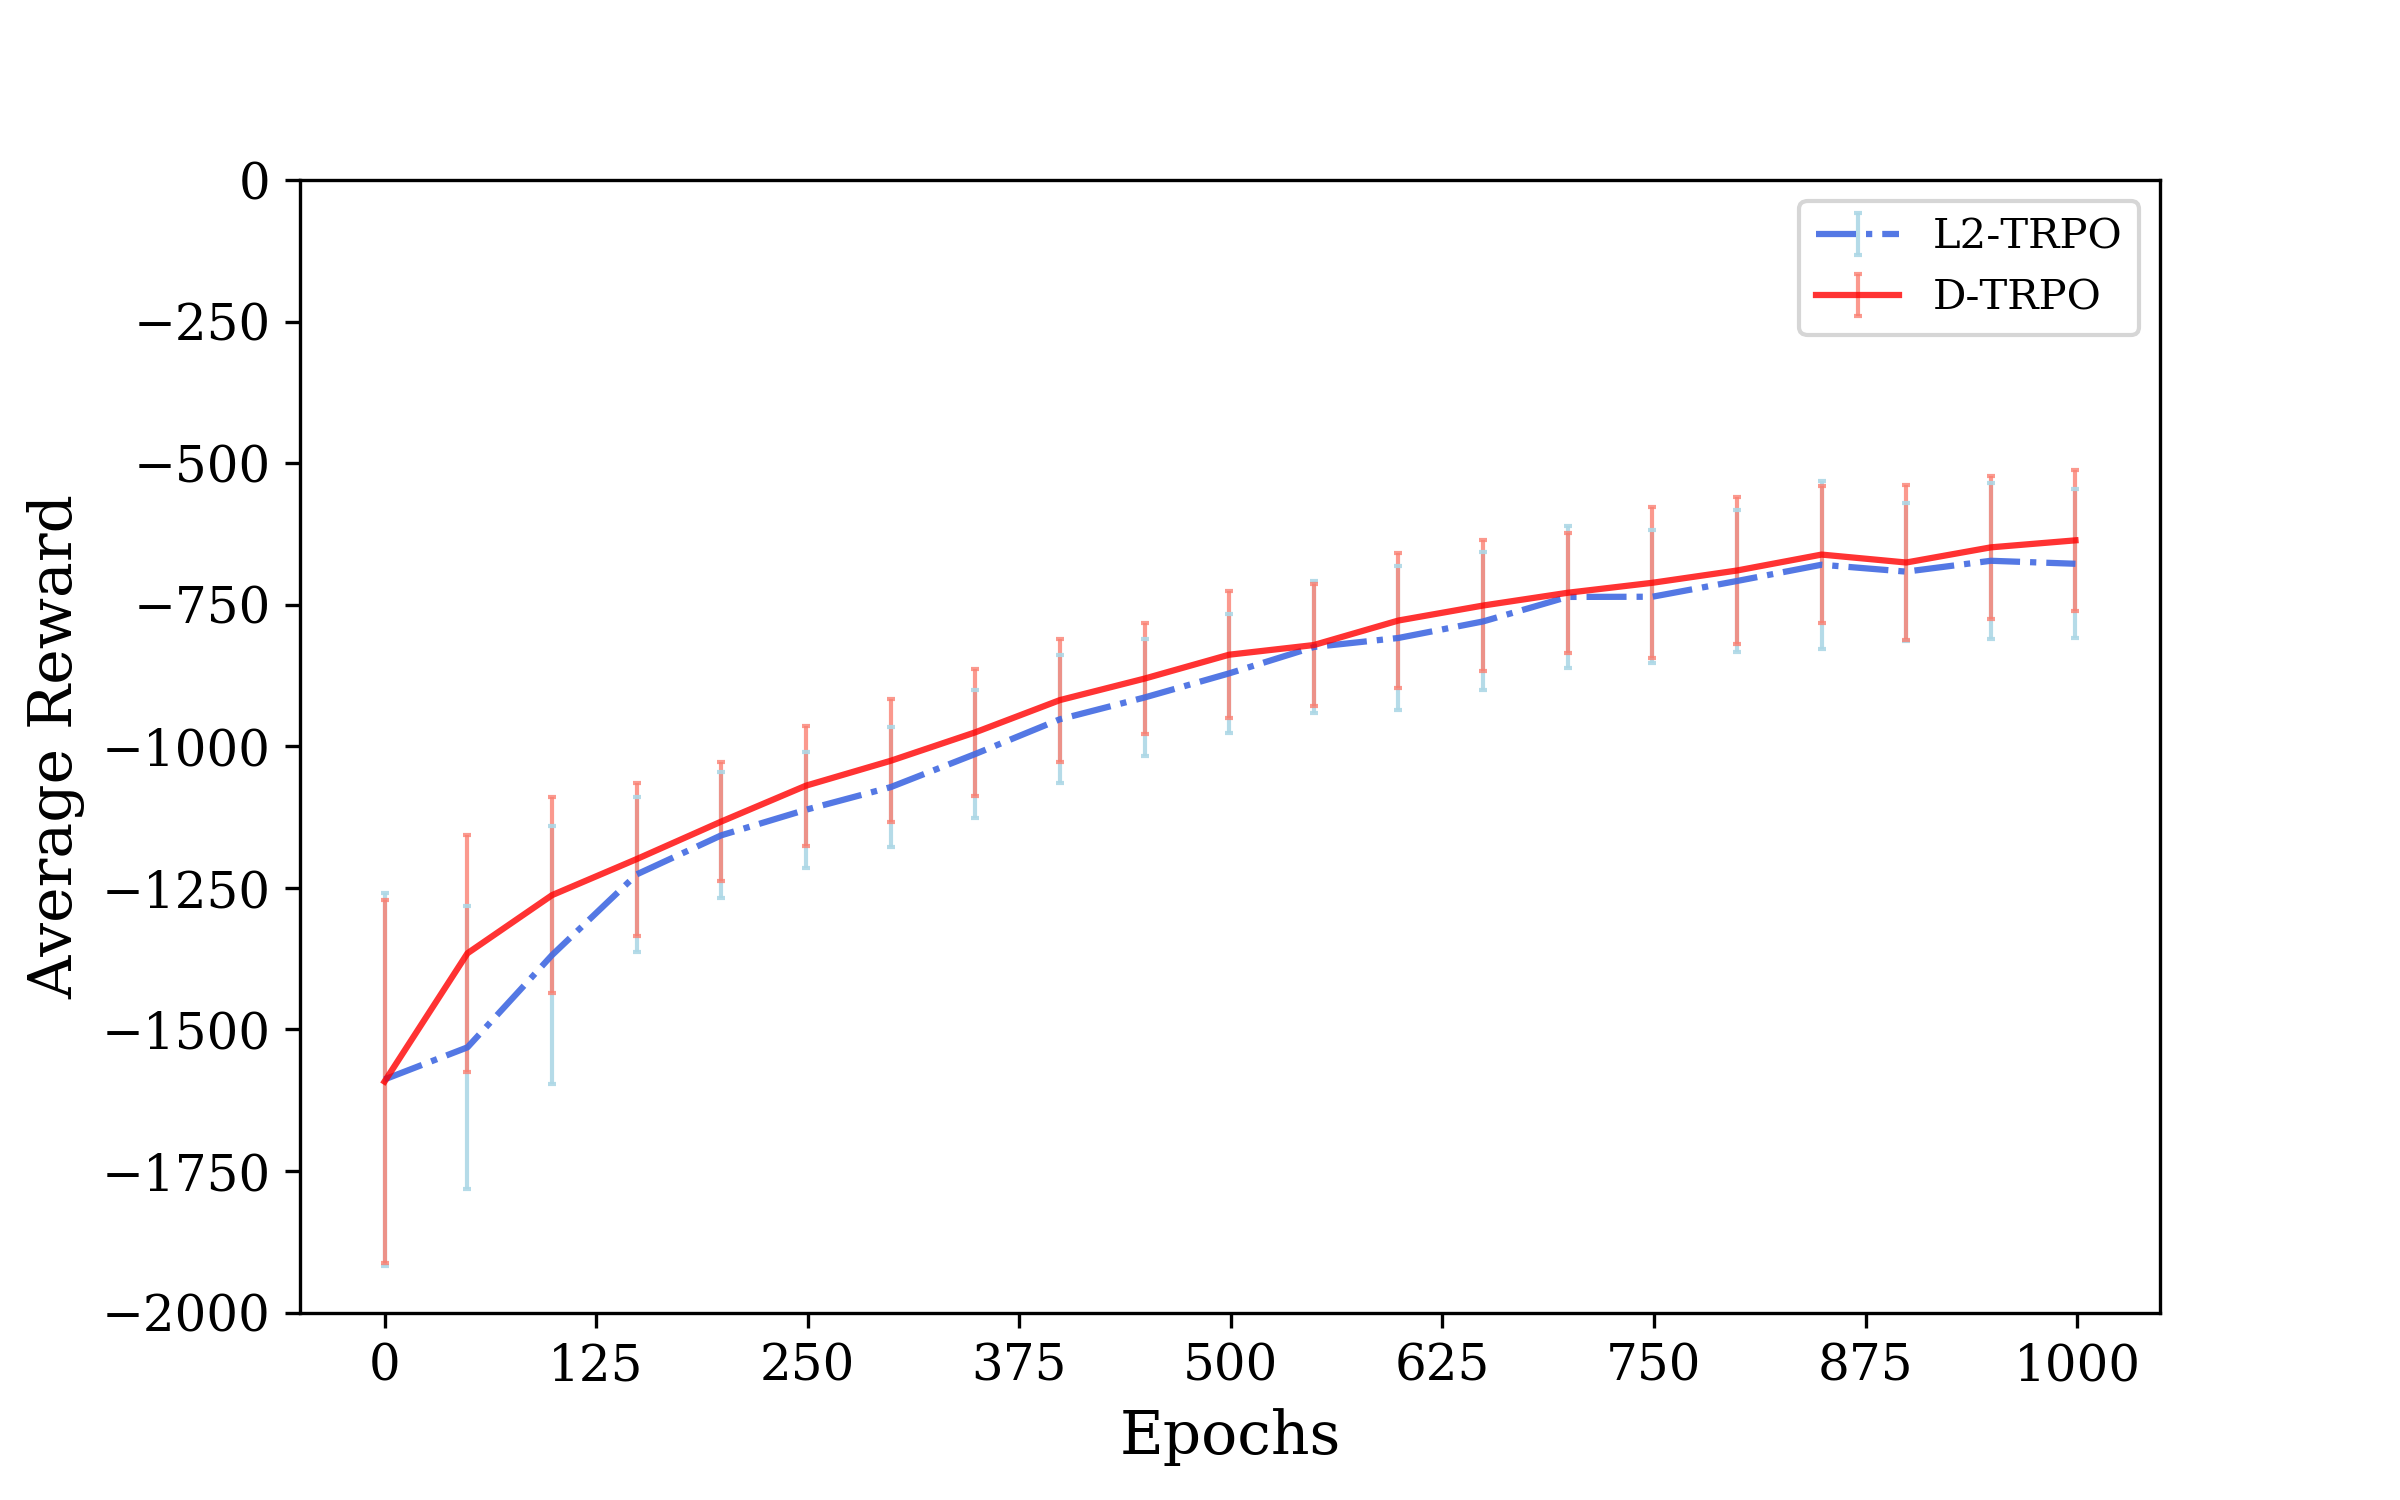
\includegraphics[width=11cm, keepaspectratio]{images/results/noises_tri_comparison_1.png}
                \caption{Training results obtained with deterministic delay of 5 steps and a Triangular perturbation.}
                \label{fig:results_tri_1}
            \end{figure}